% Ce fichier main.tex est le fichier principal \`{a} partir duquel tout est g\'{e}n\'{e}r\'{e}
% This file is the main file where the final document is generated
\documentclass{these-dbl}

% Remplir les metadonnees du pdf
% Fill the pdf metadata
\hypersetup{
   pdfauthor   = {Hongwei Zhao},
   pdftitle    = {Thesis of Hongwei},
   pdfsubject  = {Th\`{e}se de doctorat de Hongwei Zhao},
   pdfkeywords = {},
   pdfstartview= {FitV}
}

\geometry{vmargin=4.0cm}
\usepackage[intoc]{nomencl}
\usepackage{listings}
\lstset{
  language=C,
  xleftmargin=5mm,framexleftmargin=5mm,
  basicstyle=\ttfamily\small,
  keywordstyle=\color{blue},
  commentstyle=\color{gray},
  stringstyle=\color{red},
  numbers=left,
  numberstyle=\small\color{black},
  stepnumber=1,
  numbersep=5pt,
  showspaces=false,
  showstringspaces=false,
  breaklines=true,
  frame=single,
  tabsize=4,
  captionpos=b
}
\lstdefinelanguage{json}{
    basicstyle=\ttfamily\footnotesize,
    numbers=left,
    numberstyle=\tiny\color{gray},
    stepnumber=1,
    numbersep=5pt,
    showstringspaces=false,
    breaklines=true,
    frame=single,
    backgroundcolor=\color{gray!10},
    literate=
     *{0}{{{\color{blue}0}}}{1}
      {1}{{{\color{blue}1}}}{1}
      {2}{{{\color{blue}2}}}{1}
      {3}{{{\color{blue}3}}}{1}
      {4}{{{\color{blue}4}}}{1}
      {5}{{{\color{blue}5}}}{1}
      {6}{{{\color{blue}6}}}{1}
      {7}{{{\color{blue}7}}}{1}
      {8}{{{\color{blue}8}}}{1}
      {9}{{{\color{blue}9}}}{1}
      {:}{{{\color{black}:}}}{1}
      {,}{{{\color{black},}}}{1}
      {"}{{{\color{red}"}}}{1},
}
\lstdefinelanguage{python}{
  keywords={true,false,null,y,n},
  keywordstyle=\color{blue},
  basicstyle=\ttfamily\footnotesize,
  sensitive=false,
  comment=[l]{\#},
  morecomment=[l]{\#},
  commentstyle=\color{gray}\ttfamily,
  stringstyle=\color{red},
  moredelim=[l][\color{orange}]{:}
}
\makenomenclature
\renewcommand\_{\textunderscore\allowbreak}

% Spécifier vos fichiers de bibliographie
% Specify you bibliography files here
\addbibresource{./biblio/biblio.bib}
\usepackage{minitoc}

\usepackage{multirow}
\usepackage[table,xcdraw]{xcolor}
\usepackage{tabularx}
\usepackage{amssymb}
\usepackage{textgreek}
\usepackage{booktabs}
\usepackage{tabularx}
\usepackage{longtable}
\begin{document}

% Page de garde avec commande \maketitle
% Front cover calling \maketitle
% La page de garde est en français
% The front cover is in French
\selectlanguage{french}

% Inclure les infos de chaque établissement
% Include each institution data

%%% Switch case in latex
%%% https://tex.stackexchange.com/a/343306
\makeatletter
\newcommand\addcase[3]{\expandafter\def\csname\string#1@case@#2\endcsname{#3}}
\newcommand\makeswitch[2][]{%
    \newcommand#2[1]{%
        \ifcsname\string#2@case@##1\endcsname\csname\string#2@case@##1\endcsname\else#1\fi%
  }%
}
\makeatother

%%%% Il faut adapter la taille des logos dans certains cas (e.g., EGAAL, 2 etablissements)
\newcommand\hauteurlogos[3]{
    \hauteurlogoecole{#1}
    \hauteurlogoetablissementA{#2}
    \hauteurlogoetablissementB{#3}
}





%%%%%%%%%%%%%%%%%%%%%%%%%%%%%%%%%%%%%%%%%%%%%%%%%%%
%%%%%%%%%%%%%%%% ECOLES DOCTORALES %%%%%%%%%%%%%%%%

%%%% #1: dossier des images, #2: numero ED, #3: couleur ED recto, #4: couleur ED verso, #5-#6: nom complet sur plusieurs lignes
\newcommand\addecoledoctorale[6]{
    \direcole{#1}
    \numeroecole{#2}
    \definecolor{couleur-ecole-recto}{RGB}{#3}
    \definecolor{couleur-ecole-verso}{RGB}{#4}
    \nomecoleA{#5}
    \nomecoleB{#6}
}

\makeswitch[default]\ecoledoctorale{}

\addcase\ecoledoctorale{ALL}{\addecoledoctorale
    {ALL}
    {595}
    {255,165,139}
    {232,86,18}
    {Arts, Lettres, Langues}
    {}
}
\addcase\ecoledoctorale{DSP}{\addecoledoctorale
    {DSP}
    {599}
    {255,241,170}
    {255,214,12}
    {Droit et Science politiques}
    {}
}
\addcase\ecoledoctorale{EDGE}{\addecoledoctorale
    {EDGE}
    {597}
    {255,254,101}
    {255,237,0}
    {Sciences \'{e}conomiques et sciences de gestion - Bretagne}
    {}
}
\addcase\ecoledoctorale{EGAAL}{\addecoledoctorale
    {EGAAL}
    {600}
    {0,118,0}
    {0,93,49}
    {\'{E}cologie, G\'{e}osciences, Agronomie, Alimentation}
    {}
    \couleurpolice{white}
}
\addcase\ecoledoctorale{ELICCE}{\addecoledoctorale
    {ELICCE}
    {646}
    {255,207,114}
    {252,199,82}
    {\'{E}ducation, Langages, Interactions, Cognition, Clinique, Expertise}
    {}
}
\addcase\ecoledoctorale{ESC}{\addecoledoctorale
    {ESC}
    {645}
    {255,164,85}
    {240,138,0}
    {Espaces, Soci\'{e}\'{e}s, Civilisations}
    {}
}
\addcase\ecoledoctorale{MathSTICBO}{\addecoledoctorale
    {MathSTICBO}
    {644}
    {190,212,233}
    {139,181,221}
    {Math\'{e}matiques et Sciences et Technologies}
    {de l'Information et de la Communication en Bretagne Oc\'{e}ane}
}
\addcase\ecoledoctorale{MATISSE}{\addecoledoctorale
    {MATISSE}
    {601}
    {0,112,237}
    {0,84,160}
    {Math\'{e}matiques, T\'{e}l\'{e}communications, Informatique, Signal, Syst\`{e}mes,}
    {\'{E}lectronique}
    \hauteurlogos{1.8cm}{1.8cm}{1.8cm}
    \couleurpolice{white}
}
\addcase\ecoledoctorale{S3M}{\addecoledoctorale
    {S3M}
    {638}
    {159,19,90}
    {156,42,100}
    {Sciences de la Mati\`{e}re, des Mol\'{e}cules et Mat\'{e}riaux}
    {}
    \couleurpolice{white}
}
\addcase\ecoledoctorale{SML}{\addecoledoctorale
    {SML}
    {598}
    {19,139,112}
    {0,93,102}
    {Sciences de la Mer et du Littoral}
    {}
    \couleurpolice{white}
}
\addcase\ecoledoctorale{SPI}{\addecoledoctorale
    {SPI}
    {647}
    {136,191,255}
    {63,133,193}
    {Sciences pour l'Ing\'{e}nieur}
    {}
}
\addcase\ecoledoctorale{SPIN}{\addecoledoctorale
    {SPIN}
    {648}
    {161,173,255}
    {80,92,162}
    {Sciences pour l'Ing\'{e}nieur et le Num\'{e}rique}
    {}
}
\addcase\ecoledoctorale{SVS}{\addecoledoctorale
    {SVS}
    {637}
    {228,255,122}
    {200,210,0}
    {Sciences de la Vie et de la Sant\'{e}}
    {}
}





%%%%%%%%%%%%%%%%%%%%%%%%%%%%%%%%%%%%%%%%%%%%%%%%
%%%%%%%%%%%%%%%% ETABLISSEMENTS %%%%%%%%%%%%%%%%

%%%% #1 nom du logo, #2-#4: nom complet sur plusieurs lignes
\newcommand\addetablissement[4]{
    \logoetablissementB{#1}
    \nometablissementC{#2}
    \nometablissementD{#3}
    \nometablissementE{#4}
}

\makeswitch[default]\etablissement{}

\addcase\etablissement{CS}{\addetablissement
    {CS}
    {}
    {}
    {CentraleSup\'{e}lec}
}
\addcase\etablissement{EHESP}{\addetablissement
    {EHESP}
    {}
    {l'\'{E}cole des Hautes \'{E}tudes}
    {en Sant\'{e} Publique}
    \hauteurlogos{2cm}{}{2.5cm}
}
\addcase\etablissement{ENIB}{\addetablissement
    {ENIB}
    {}
    {}
    {l'\'{E}cole Nationale d'Ing\'{e}nieurs de Brest}
}
\addcase\etablissement{ENS}{\addetablissement
    {ENS}
    {}
    {}
    {l'\'{E}cole Normale Sup\'{e}rieure de Rennes}
}
\addcase\etablissement{ENSAI}{\addetablissement
    {ENSAI}
    {}
    {l'\'{E}cole Nationale de la Statistique}
    {et de l'Analyse de l'Information}
}
\addcase\etablissement{ENSCR}{\addetablissement
    {ENSCR}
    {}
    {l'\'{E}cole Nationale Sup\'{e}rieure}
    {de Chimie Rennes}
}
\addcase\etablissement{ENSTA}{\addetablissement
    {ENSTA}
    {}
    {l'\'{E}cole Nationale Sup\'{e}rieure}
    {de Techniques Avanc\'{e}es Bretagne}
}
\addcase\etablissement{IMTA}{\addetablissement
    {IMTA}
    {l'\'{E}cole Nationale Sup\'{e}rieure}
    {Mines-T\'{e}l\'{e}com Atlantique Bretagne}
    {Pays de la Loire -- IMT Atlantique}
}
\addcase\etablissement{INSA}{\addetablissement
    {INSA}
    {}
    {l'Institut National des}
    {Sciences Appliqu\'{e}es de Rennes}
    \hauteurlogos{1.8cm}{}{2cm}
}
\addcase\etablissement{InstitutAgro}{\addetablissement
    {InstitutAgro}
    {}
    {}
    {l'Institut Agro Rennes Angers}
}
\addcase\etablissement{UBO}{\addetablissement
    {UBO}
    {}
    {}
    {l'Universit\'{e} de Bretagne Occidentale}
}
\addcase\etablissement{UBS}{\addetablissement
    {UBS}
    {}
    {}
    {l'Universit\'{e} Bretagne Sud}
}
\addcase\etablissement{UR}{\addetablissement
    {UR}
    {}
    {}
    {l'Universit\'{e} de Rennes}
}
\addcase\etablissement{UR2}{\addetablissement
    {UR2}
    {}
    {}
    {l'Universit\'{e} Rennes 2}
}

%%%% #1-#2: nom des deux logos, #3-#7: nom complet de la double affiliation sur plusieurs lignes
\newcommand\addpairetablissements[7]{
    \logoetablissementA{#1}
    \logoetablissementB{#2}
    \nometablissementA{#3}
    \nometablissementB{#4}
    \nometablissementC{#5}
    \nometablissementD{#6}
    \nometablissementE{#7}
}

% ALL, ESC: ENSAB-UR2
\addcase\etablissement{ENSAB-UR2}{\addpairetablissements
    {ENSAB}
    {UR2}
    {}
    {l'\'{E}cole Nationale Sup\'{e}rieure}
    {d'Architecture de Bretagne}
    {d\'{e}livr\'{e}e conjointement avec}
    {l'Universit\'{e} Rennes 2}
    \hauteurlogos{2cm}{1.2cm}{2cm}
}
% DSP, MATISSE, SVS: UR2-UR
\addcase\etablissement{UR2-UR}{\addpairetablissements
    {UR2}
    {UR}
    {}
    {}
    {l'Universit\'{e} Rennes 2}
    {d\'{e}livr\'{e}e conjointement avec}
    {l'Universit\'{e} de Rennes}
    \hauteurlogos{1.8cm}{1.8cm}{1.5cm}
}
% DSP, EDGE: EHESP-UR
\addcase\etablissement{EHESP-UR}{\addpairetablissements
    {EHESP}
    {UR}
    {}
    {l'\'{E}cole des Hautes \'{E}tudes}
    {en Sant\'{e} Publique}
    {d\'{e}livr\'{e}e conjointement avec}
    {l'Universit\'{e} de Rennes}
    \hauteurlogos{2cm}{2cm}{1.5cm}
}
% MATISSE: InstitutAgro-UR
\addcase\etablissement{InstitutAgro-UR}{\addpairetablissements
    {InstitutAgro}
    {UR}
    {}
    {l'Institut Agro}
    {Rennes Angers}
    {d\'{e}livr\'{e}e conjointement avec}
    {l'Universit\'{e} de Rennes}
    \hauteurlogos{1.8cm}{1.2cm}{1.2cm}
}
% SPI: ENIB-UBO
\addcase\etablissement{ENIB-UBO}{\addpairetablissements
    {ENIB}
    {UBO}
    {}
    {l'\'{E}cole Nationale}
    {d'Ing\'{e}nieurs de Brest}
    {d\'{e}livr\'{e}e conjointement avec}
    {l'Universit\'{e} de Bretagne Occidentale}
    \hauteurlogos{2cm}{1.6cm}{1.6cm}
}


% Inclure infos de l'école doctorale
% Include doctoral school data
\ecoledoctorale{MathSTICBO}

% Inclure infos de l'établissement
% Include institution data
\etablissement{UBS}

%Inscrivez ici votre sp\'{e}cialit\'{e} (voir liste des sp\'{e}cialit\'{e}s sur le site de votre \'{e}cole doctorale)
%Indicate the domain (see list of domains in your ecole doctorale)
\spec{Informatique et Architectures Numériques}

%Attention : le pr\'{e}nom doit être en minuscules (Jean) et le NOM en majuscules (BRITTEF) 
%Attention : the first name in small letters and the name in Capital letters 
\author{Hongwei ZHAO}

% Donner le titre complet de la th\`{e}se, \'{e}ventuellement le sous titre, si n\'{e}cessaire sur plusieurs lignes 
%Give the complete title of the thesis, if necessary on several lines
\title{Étude et conception d'architectures de communication sous contraintes pour les systèmes sur puce}
\lesoustitre{Study and design of constrained communication architecturess for systems-on-a-chip}

%Indiquer la date et le lieu de soutenance de la th\`{e}se 
%indicates the date and the place of the defense 
\date{xx/xx/2025}
\lieu{Lorient}

%Indiquer le nom du (ou des) laboratoire (s) dans le(s)quel(s) le travail de th\`{e}se a \'{e}t\'{e} effectu\'{e}, indiquer aussi si souhait\'{e} le nom de la (les) facult\'{e}(s) (UFR, \'{e}cole(s), Institut(s), Centre(s)...), son (leurs) adresse(s)... 
%Indicates the name (or names) of research laboratories where the work has been done as well as (if desired) the names of faculties (UFR, Schools, institution...
\uniterecherche{UMR CNRS 6285, Lab-STICC, Université Bretagne Sud}

%Indiquer le Numero de th\`{e}se, si cela est opportun, ou laisser vide pour faire disparaitre cet ligne de la couverture
%Indicate the number of the thesis if there is one. otherwise leave empty so the line disappeurs on the cover

%\numthese{??} % \numthese{}

%Indiquer le Pr\'{e}nom en minuscules et le Nom en majuscules, le titre de la personne et l’\'{e}tablissement dans lequel il effectue sa recherche  
%Indicates the first name on small letters and the Names on capital letters, the person's title and the institution where he/she belongs to.
%Exemples :  Examples :
%%%- Professeur, Universit\'{e} d’Angers 
%%%- Chercheur, CNRS, \'{e}cole Centrale de Nantes 
%%%-  Professeur d’universit\'{e} – Praticien Hospitalier, Universit\'{e} Paris V  
%%%-  Maitre de conf\'{e}rences, Oniris 
%%%- Charg\'{e} de recherche, INSERM, HDR, Universit\'{e} de Tours  
 %S’il n’y a pas de co-direction, faire disparaitre cet item de la couverture  
 %In there is no co-director, remove the item from the cover
\jury{
{\normalTwelve \textbf{Rapporteur\textperiodcentered trice\textperiodcentered s avant soutenance :}}\\ \newline
\footnotesizeTwelve
\begin{tabular}{@{}ll}
Jean-Max Dutertre & Professeur des Universités (Ecole des Mines de Saint-Etienne) \\
Guillaume Bouffard & Chercheur (ANSSI and Information Security Group, ENS) \\
\end{tabular}

\vspace{\baselineskip}
{\normalTwelve \textbf{Composition du Jury :}}\\
\newline
\footnotesizeTwelve
\begin{tabular}{@{}lll}
Pr\'{e}sident: & Lionel Torres & Professeur des Universités (Polytech Montpellier, Université Montpellier)  \\
Examinateur: & Karine Heydemann & Maitre de Conférence HDR (Sorbonne Université) \\
Dir. de th\`{e}se: & Guy Gogniat & Maitre de Conférence HDR (Lab-STICC, Université Bretagne Sud) \\
Co-dir. de th\`{e}se: & Vianney Lap\^{o}tre & Professeur des Universités (Lab-STICC, Université Bretagne Sud) \\
\end{tabular}
}

\maketitle

% Sélectionner la langue du contenu suivant cette ligne
% Select the content language following this line
\selectlanguage{french}
\selectlanguage{english}

\thispagestyle{empty}
\pagenumbering{roman}

% Inclusion du chapitre remerciement
% Input acknowledgement chapter
\clearemptydoublepage
\chapter*{Acknowledgement}

Je tiens à exprimer ma profonde gratitude à toutes les personnes qui ont contribué de près ou de loin à l’aboutissement de cette thèse.

Je remercie tout d’abord mes directeurs de thèse, Guy Gogniat et Vianney Lapôtre, pour leur encadrement, leur patience, leur conseils précieux et leur soutien constant tout au long de ces années. Leur rigueur scientifique et leur bienveillance ont été pour moi une source d’inspiration.

Je souhaite également remercier mes collègues de laboratoire, Kévin Queneherve, Adam Henault, Gwenn le Conidec, Tianxu Li pour leur collaboration et leur bonne humeur, en particulier ceux qui m’ont accompagné dans les moments clés de mes travaux de recherche. Un grand merci aux collègues de l’accueil, Emmanuel barret et Beatrice Guern de la cellule informatique et du service scolarité, pour leur efficacité et leur aide précieuse dans la gestion des aspects pratiques et administratifs de mon séjour au laboratoire.

Je n’oublie pas non plus mes anciens collègues, William Pensec, Mohamed El Bouazzati, Kamel Aizi et Nicolas Gaudin qui ont marqué le début de mon parcours de recherche et ont contribué à mon développement professionnel et personnel.

Mes pensées les plus sincères vont à mes parents, pour leur amour inconditionnel, leur soutien moral et leur confiance inébranlable en moi. Sans eux, rien de tout cela n’aurait été possible.

Enfin, je remercie chaleureusement les organismes ayant financé ma thèse, ARED RB COMSEC et DGA. Leur soutien a été essentiel pour mener à bien ce travail dans de bonnes conditions.

% Ne pas oublier cette commande qui g\'{e}n\`{e}re la page de couverture avant
% This command will generate the front cover
\frontmatter
\clearemptydoublepage
\dominitoc

\newpage
\phantomsection
\renewcommand{\contentsname}{Table of Contents}
\addcontentsline{toc}{chapter}{Table of Contents}
\tableofcontents %sommaire %table of content
%\shorttableofcontents{Sommaire}{0}

\clearemptydoublepage
\pagenumbering{arabic}
\setcounter{page}{1}
\setcounter{mtc}{6}
\mainmatter
\chapter*{Introduction}
\addcontentsline{toc}{chapter}{Introduction}
\chaptermark{Introduction}

Embedded systems have become an integral part of modern technology, powering a wide range of applications from consumer electronics and industrial control to automotive systems and critical infrastructures. Their widespread adoption is driven by their ability to deliver dedicated functionality with efficiency, compact size, and relatively low cost. As these systems continue to proliferate and play essential roles in safety-critical and real-time applications, their reliability and security have become increasingly important concerns. Faults—whether caused by hardware defects, environmental conditions, or malicious interference—can lead to severe consequences, including system crashes, data corruption, or even catastrophic failures in mission-critical scenarios~\cite{bar2006sorcerer} \cite{karaklajic2013hardware}. Therefore, ensuring the correctness and resilience of embedded systems has emerged as a vital area of research within both academia and industry.

One crucial aspect of system resilience is the identification and mitigation of potential vulnerabilities. Traditional fault tolerance strategies address CPU-level execution errors and memory corruption,  For instance, the work in ~\cite{Shukla2023An} introduces a novel parity-based fault-tolerant instruction decoder architecture tailored for dual-core processors implemented on FPGAs. Similarly,\cite{Ramos2018Efficient} proposes a low-overhead, parity-based technique to protect the register file in RISC-V soft processors on Xilinx FPGAs, leveraging implementation redundancy and validating its efficacy through fault injection experiments. In another direction \cite{Medwed2011Arithmetic} presents efficient ALU architectures utilizing multi-residue codes to achieve high error detection capabilities. The proposed methods minimize error weight and are shown to have a minimal performance impact in typical smart card applications, with detailed trade off analysis in terms of area and critical path delay. Recent research has shown that other components—particularly the on-chip communication infrastructure such as system buses—are also susceptible to faults and attacks. Despite the vital role system buses play in facilitating data transfer between processing units, memory, and peripherals, they are often neglected in security and reliability discussions. This oversight constitutes a significant blind spot in the comprehensive protection strategy of embedded systems.

Moreover, as attack surfaces continue to expand, adversaries are becoming increasingly sophisticated, targeting non-traditional vectors such as fault injection and side-channel manipulation to compromise system integrity. Among these, bus-level attacks have attracted growing attention due to their ability to disrupt communication, intercept data in transit, or inject malicious payloads—often without requiring direct access to the CPU. In~\cite{mishra2024faults}, the authors demonstrate the use of electromagnetic pulse (EMP) injections to compromise the ARM TrustZone by targeting the bus. Unlike the work proposed in this manuscript, their solution relies on a software-based countermeasure, which is not evaluated for the potential introduction of new vulnerabilities. Furthermore, their work does not analyze overhead, execution time, or the increase in program complexity relative to the original implementation. Despite the central role of interconnect networks in System-on-Chip (SoC) architectures, both logical and physical attacks on these components remain underexplored. Addressing this critical gap is the primary objective of the present work.

This study advances the field by conducting an in-depth analysis of the three bus architectures~\cite{mitic2006survey}, systematically identifying potential vulnerabilities within the bus communication system (Wishbone, AXI-Lite, AXI). Furthermore, for the Wishbone bus, building upon prior work that demonstrates the feasibility of bus-level attacks~\cite{zhao2024communication}, we introduce a comprehensive hardware-based countermeasure specifically designed to defend against such threats, underscoring the insufficiency of software-only solutions. In addition, we perform a comparative analysis of existing countermeasures, illustrating the limitations of alternative approaches and demonstrating the superior effectiveness of our proposed hardware solution in ensuring robust and reliable system protection.

\section*{Contributions}
\addcontentsline{toc}{section}{Contributions}

This thesis makes the following key contributions to the advancement of secure System-on-Chip (SoC) design, particularly in the context of defending on-chip communication infrastructures against emerging fault injection and bus-level attacks:

\begin{enumerate}
\item Comprehensive analysis of bus architectures: We perform a detailed architectural and functional analysis of three widely used on-chip communication protocols—Wishbone, AXI-Lite, and AXI. By examining their transaction models, signal structures, and timing behaviors, we identify structural and design-level properties that may expose them to fault injection, bus snooping, and data hijacking attacks.

\item Vulnerability identification across multiple bus systems: Through systematic evaluation, we uncover previously underexplored vulnerabilities in each of the three bus systems. These include weak or absent integrity checks, unprotected data paths, and susceptibility to transient fault propagation—especially in unsecured or resource-constrained SoC environments.

\item Countermeasure evaluation for the Wishbone bus: We conduct a comparative study of existing countermeasures applicable to the Wishbone bus, including both software-based and hybrid techniques. Our analysis highlights the trade-offs between security coverage, performance overhead, and implementation complexity. We show that software-only approaches are insufficient for high-assurance applications due to limitations in fault detection granularity and real-time response.

\item Design and implementation of a hardware-based countermeasure: As a core contribution, we design a novel hardware-based countermeasure for the Wishbone bus that provides full-spectrum protection against bus-level attacks. Our approach integrates parity-based error detection, signal redundancy, and protocol monitoring logic to defend against both logical and physical attacks. Experimental results demonstrate that the proposed solution offers robust security with minimal performance and area overhead, making it suitable for FPGA-based and resource-constrained embedded systems.
\end{enumerate}

\section*{Organisation of document}
\addcontentsline{toc}{section}{Organisation of document}

This thesis is organized into five chapters. Chapter 1 introduces the context of system-level attacks in SoCs, defining hardware and software fault injection methods and presenting countermeasure classifications. Chapter 2 describes the experimental setup, including SoC construction using LiteX, bus configurations, fault models, benchmarks, and attacker assumptions. Chapter 3 focuses on vulnerability exploitation in the Wishbone bus, AXI and AXI-Lite buses. Chapter 4 evaluates both software and hardware countermeasures in the Wishbone bus, comparing their effectiveness, and proposing a custom hardware-based solution. Finally, Chapter 5 summarizes the main contributions and outlines directions for future work.

\section*{Publications}

During the course of the Ph.D., I actively presented my research at several international and national scientific events:
\begin{itemize}
    \item I delivered an oral presentation at the IEEE International Conference on Cyber Security and Resilience (CSR), held in London, UK, where I also published the peer-reviewed paper entitled “Communication Architecture Under Siege: An In-depth Analysis of Fault Attack Vulnerabilities and Countermeasures”. This work focused on fault injection vulnerabilities in SoC communication infrastructures and proposed a multi-layered countermeasure framework.
    \item I presented a poster at the JAIF 2023 (Journée thématique sur les attaques par injection de fautes), held in Gardanne, France. The poster showcased preliminary results on fault propagation behaviors across bus architectures, contributing to the national dialogue on fault injection resistance in embedded systems.
    \item I also participated in the GDR SoC 2025 Workshop in Lorient, France, where I gave a poster presentation summarizing recent advances in fault-tolerant communication protocols and discussed future integration into secure SoC designs.
\end{itemize}








\clearemptydoublepage

\clearemptydoublepage
\chapter{Attacks}
This chapter provides a comprehensive overview of system-level security threats in embedded systems. It begins by defining the concept of an attack and distinguishes between two primary categories: software attacks, which exploit vulnerabilities in code or system logic, and hardware attacks, which target the physical components of a system. 
\section{Definition}
With the rapid proliferation of embedded electronic systems in critical applications—ranging from automotive control units~\cite{7917080} and medical devices~\cite{4431854} to industrial automation and consumer electronics—their security has become a major concern. These systems often operate in environments where reliability and integrity are paramount, yet they are increasingly exposed to various threat vectors. As embedded systems grow in complexity and connectivity, they become attractive targets for attackers seeking to compromise system behavior, extract sensitive data, or cause functional disruption.

In this context, an attack is defined as any intentional act aimed at lowering the security level of an embedded system. Such acts may violate one or more core security properties: confidentiality, integrity, or availability. Attacks can be carried out through diverse methods, depending on the adversary’s access level, knowledge, and objectives. The origins of attacks in embedded systems trace back to early fault-tolerance~\cite{9684471} research, where hardware faults were studied for reliability purposes—later repurposed by adversaries as vectors for deliberate disruption. Over time, both hardware and software dimensions of these systems have revealed exploitable vulnerabilities.

Attacks are generally classified into two major categories: hardware attacks \cite{6856140} and software attacks \cite{6832045}. As Figure\ref{tree} shows, hardware attacks target the physical components of a system and include techniques such as fault injection, side-channel analysis, and probing. A comparison between hardware attacks and software Attack is shown in Table\ref{hw sw}. These methods typically require physical access but can be highly effective in bypassing traditional protections. Software attacks, on the other hand, exploit weaknesses in code, configuration, or system logic—examples include buffer overflows, code injection, and control-flow hijacking. Despite the differing methods, both types can produce system-wide effects and are therefore studied collectively under the broader category of system-level attacks.

\begin{figure}[t!]
  \centering
  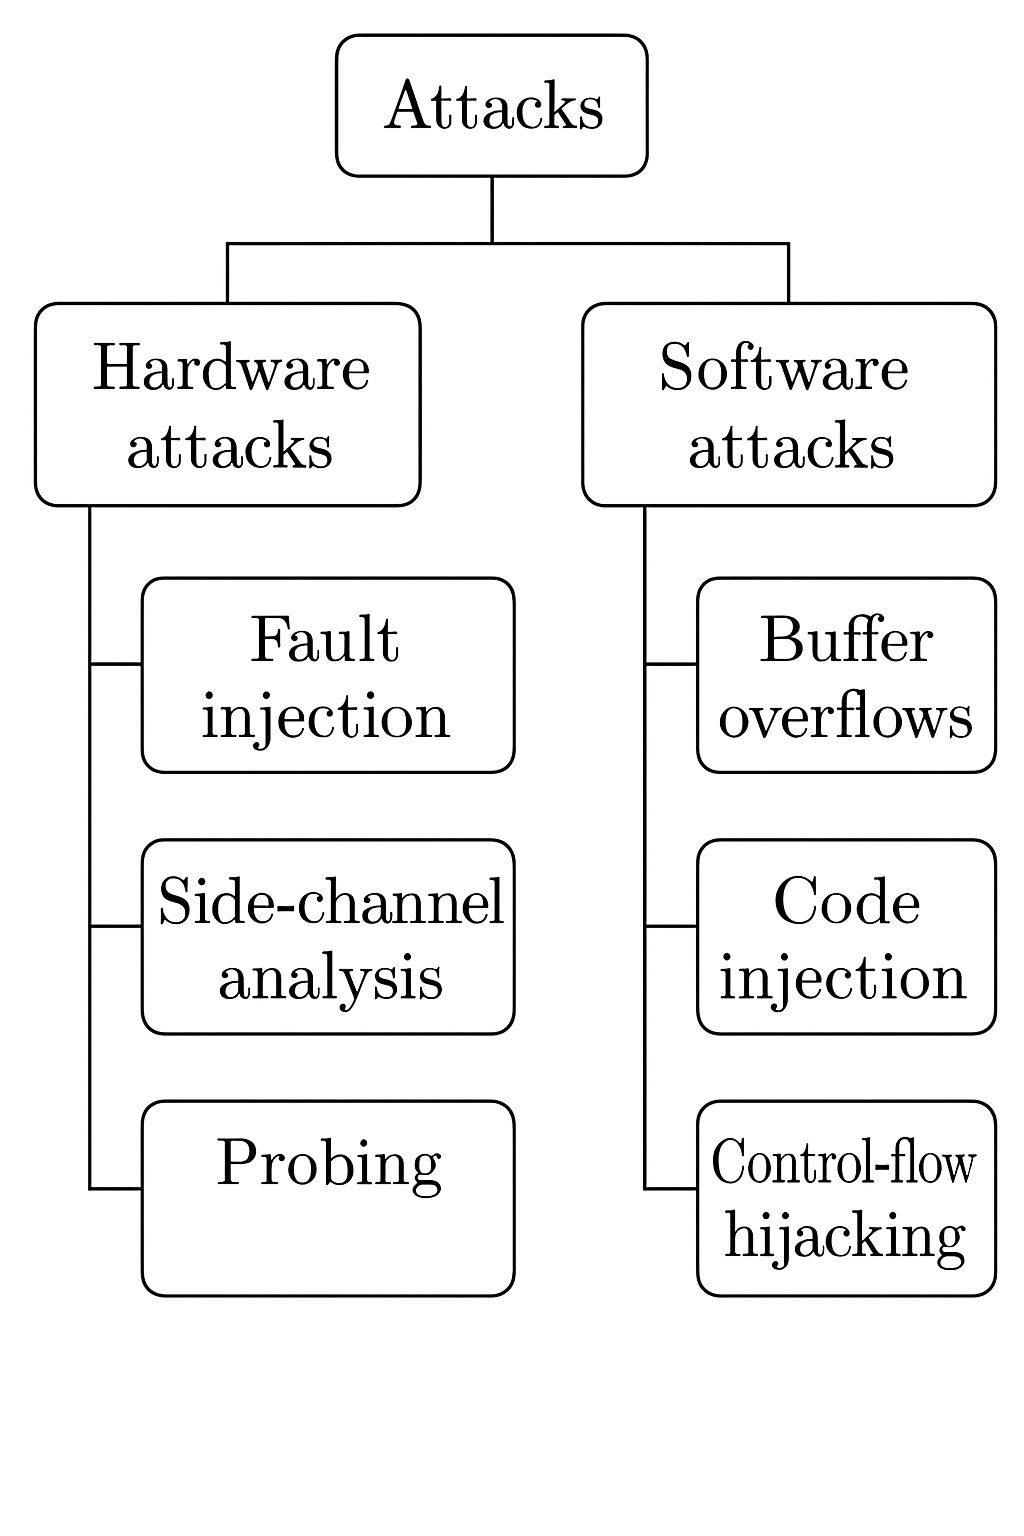
\includegraphics[width=0.5\linewidth]{Chapitre1/figures/tree.png}
  \caption{Classification of attacks into hardware and software categories, with representative techniques for each}
  \label{tree}
\end{figure}

\begin{table}[htbp]
\caption{Comparison of characteristics between hardware attack and software attack}
\label{hw sw}
\centering
\begin{tabularx}{\textwidth}{lXX}
\toprule
Aspect          & Hardware Attack                                          & Software Attack                                    \\
\midrule
Target Layer    & Physical components (CPU, memory, bus)                   & Software stack (code, memory, OS)                  \\
Access Method   & Requires physical or near-physical access                & Often remote, via crafted inputs or interfaces     \\
Techniques      & Fault injection, side-channel, probing                   & Buffer overflow, code injection, control hijacking \\
Detectability   & Hard to detect; minimal digital footprint                & Easier to monitor with logs and security tools     \\
Countermeasures & Costly and hard to retrofit; involve hardware redundancy & Easier to update via patches and software defenses \\
Typical Use     & Cryptographic key extraction, device tampering           & Privilege escalation, malware deployment           \\
\bottomrule
\end{tabularx}
\end{table}

\section{Software attack}
\subsection{Introduction and Classification}
In the domain of embedded and cyber-physical systems, software attacks \cite{6832002} constitute one of the most prevalent and evolving classes of security threats. Unlike hardware-based attacks, which typically require physical proximity or invasive access to a device, software attacks exploit logical vulnerabilities in code, configuration, or execution flow to subvert system behavior, escalate privileges, or extract sensitive data. These attacks are particularly insidious due to their ease of propagation, adaptability, and potential to be launched remotely.

From a classification perspective, software attacks on embedded systems can be categorized based on the attack vector, operational phase, or targeted system component. Broadly speaking, these can be delineated into:

\textbf{Code-level attacks}, such as memory corruption~\cite{1467812} and buffer overflows~\cite{821514}, exploit programming errors in memory management. These vulnerabilities allow attackers to manipulate control data structures—such as return addresses as shown in Figure \ref{buffer} or function pointers—to hijack the execution flow or inject arbitrary code. Since many embedded systems are implemented in memory-unsafe languages like C, these attacks remain a prevalent and potent threat.

\begin{figure}[t!]
  \centering
  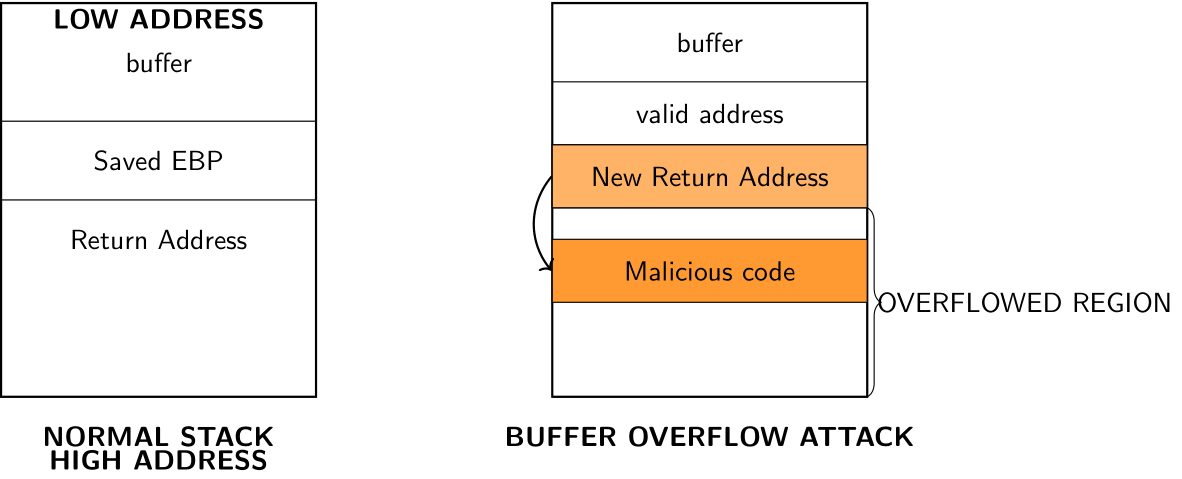
\includegraphics[width=0.5\linewidth]{Chapitre1/figures/buffer overflow.png}
  \caption{Principle of buffer overflow in program}
  \label{buffer}
\end{figure}

\textbf{System-level attacks} aim at compromising the trusted computing base of the system by targeting components such as operating system calls~\cite{9251949}, kernel modules~\cite{chen2011linux} and device drivers~\cite{yuce2018fault}, as shown in Figure\ref{system}. By exploiting these privileged layers, adversaries can gain access to critical resources, override security policies, or disable protection mechanisms entirely. These attacks are particularly dangerous due to their deep integration with the system architecture and wide-reaching consequences.

\begin{figure}[t!]
  \centering
  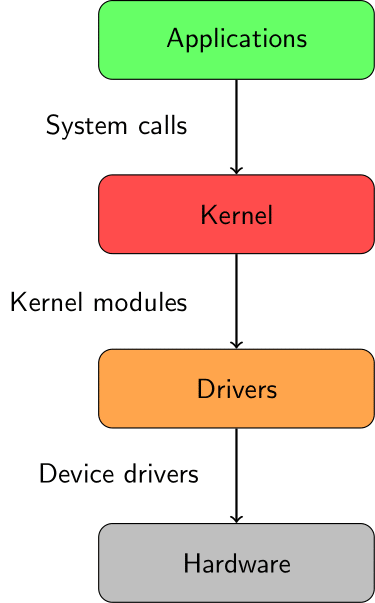
\includegraphics[width=0.5\linewidth]{Chapitre1/figures/system.png}
  \caption{Different system-level attack aspects}
  \label{system}
\end{figure}

\textbf{Firmware manipulation} involves tampering with the low-level binary code responsible for device initialization and hardware configuration. Typical targets include bootloaders~\cite{redini2017bootstomp} and embedded system images~\cite{ling2023adversarial}, which can be modified to introduce persistent malicious behavior as Figure \ref{Firmware} shows. Firmware-level attacks are often stealthy and durable, capable of surviving system resets and bypassing runtime protections.

\begin{figure}[t!]
  \centering
  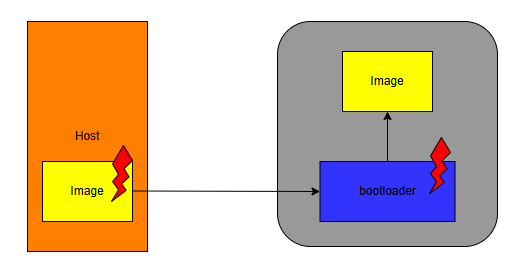
\includegraphics[width=0.5\linewidth]{Chapitre1/figures/Firmware.png}
  \caption{Firmware manipulation on bootloader and embedded system image}
  \label{Firmware}
\end{figure}

\textbf{Malicious configuration} and \textbf{runtime reprogramming} represent another class of attacks that do not directly alter code but instead manipulate system behavior by changing initialization values, parameter tables, or control logic at runtime~\cite{sinanovic2017analysis, alam2020soft}. As the Figure shows, the attacker can change initial value of a as 4,  These methods can bypass traditional integrity checks and allow adversaries to exploit dynamic features of embedded systems, such as reconfigurability or exposed debugging interfaces.

\begin{figure}[t!]
  \centering
  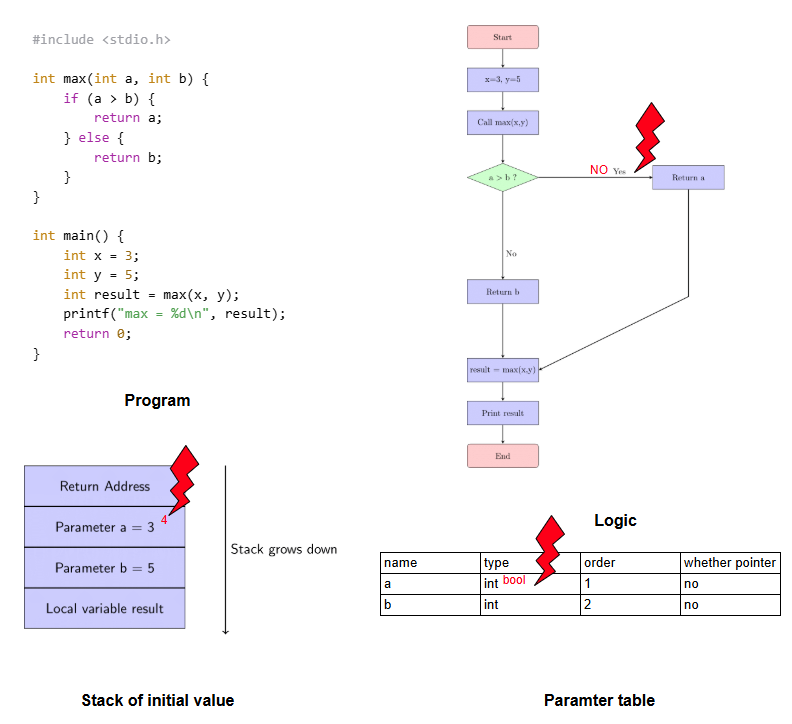
\includegraphics[width=0.5\linewidth]{Chapitre1/figures/malicious.png}
  \caption{Malicious configuration by changing initialization values, parameter tables and control logic}
  \label{malicious}
\end{figure}

\textbf{Application-level exploitation} targets flaws in application logic or communication interfaces. Common techniques include exploiting improper input validation~\cite{hayati2008modeling}, abusing insecure update procedures~\cite{alhamed2013stacking}, or leveraging weak authentication mechanisms. These attacks often serve as entry points for more persistent compromises, especially in systems that lack isolation between application and system layers.

Each class of software attack can be further analyzed along several dimensions, allowing for a more structured understanding of their mechanisms and implications. One key dimension is the attacker’s knowledge model, which refers to the level of internal system knowledge available to the adversary. In a black-box model, the attacker has no information about the system’s internal architecture or behavior and relies solely on observed input-output relationships. In contrast, the white-box model assumes complete knowledge of the system, including source code, memory layout, and execution environment. The gray-box model lies in between, where partial information is available—such as known APIs or hardware specifications—allowing for more targeted attacks without full system access.

Another important classification criterion is the delivery method of the attack. Software attacks may be introduced through various channels, depending on system accessibility and vulnerability exposure. These include over-the-air updates, which can be exploited to inject malicious firmware or configuration changes; local scripts or binaries, often executed through command-line interfaces or operating system vulnerabilities; and interface fuzzing, where malformed or randomized inputs are sent to system interfaces (e.g., I/O ports, communication buses, or APIs) to trigger unintended behaviors.

Finally, software attacks can also be distinguished by their persistence goal. Some aim for temporary disruption, such as inducing transient faults or causing momentary denial-of-service conditions \cite{7081075}. Others pursue long-term compromise, seeking to establish persistent control over the system—for example, by injecting backdoors \cite{tol2022toward}, modifying firmware \cite{bettayeb2019firmware}, or escalating privileges \cite{davi2010privilege}.

Understanding this multi-dimensional taxonomy of software attacks is essential for several reasons. It enables the development of more comprehensive threat models, facilitates risk assessment at different levels of the system, and informs the design of tailored defense mechanisms that can address a wider spectrum of threats across different attack surfaces and adversary capabilities.

\subsection{Attack Methodologies}
Software attacks exploit logical vulnerabilities, design flaws, or execution behaviors within a system’s software stack to compromise confidentiality, integrity, or availability. These attacks often bypass hardware-level defenses by manipulating code execution, system memory, or control flow at various abstraction levels. Over the past decades, software attack methodologies have evolved in sophistication—from early buffer overflows to modern fault-induced logic corruption—driven by advancements in both attack tools and target complexity.

One of the most fundamental classes of software attacks involves control-flow manipulation, where an adversary seeks to alter the intended execution path of a program. Techniques such as return-oriented programming (ROP)\cite{checkoway2010return}, jump-oriented programming (JOP)\cite{bletsch2011jump}, and function pointer hijacking \cite{bertani2023untangle} allow attackers to redirect the flow of execution without injecting new code. These methods rely on the ability to overwrite stack or heap structures, often through memory corruption vulnerabilities like buffer overflows or use-after-free conditions.

Closely related are code injection attacks, where malicious code is introduced into the memory space of a running process. Historically, these attacks were prevalent in systems lacking execution protection (e.g., DEP\cite{isawa2013generic}/NX\cite{werner2016no}), where attacker-controlled data could be both written and executed. While modern architectures implement various memory protections, code injection remains feasible when combined with information leakage or runtime reconfiguration, such as just-in-time (JIT) spraying \cite{chen2013jitsafe} or script-based code assembly \cite{wang2013metasymploit}.

Another important category includes privilege escalation \cite{davi2010privilege} and logical bypass attacks \cite{xu2017novel}, where adversaries exploit incorrect access control implementations or faulty assumptions in system logic. These attacks may be local—e.g., escalating from user to kernel space—or remote, targeting web-based interfaces or firmware. A fault injection at the software level, such as skipping an authentication check or corrupting return values, can directly result in unauthorized privilege gains.

An increasingly relevant methodology involves fault-assisted software attacks \cite{yuce2018fault}, which blur the boundary between physical disturbance and logical manipulation. By inducing faults—via electromagnetic pulses, clock/voltage glitches, or even rowhammer-style memory perturbations—attackers can corrupt specific instructions, modify control variables, or cause inconsistent system states. This type of attack has been successfully used to bypass cryptographic checks, tamper with authentication logic, or induce incorrect branching decisions. Importantly, such attacks exploit the dynamic behavior of executing software rather than static vulnerabilities.

Micro-architectural exploitation, including techniques like Spectre, Meltdown, and more recently transient execution attacks, represents another powerful software-level methodology. These attacks leverage speculative execution and cache side-effects to leak data across security boundaries, without violating any formal access rules. Although the attack surface lies in software instructions, the underlying vulnerabilities are deeply rooted in hardware optimizations, making them challenging to fully mitigate.

Additionally, software fault injection (SFI) frameworks \cite{9251063} have been developed not only for testing purposes but also as practical tools for controlled attack simulation. These frameworks can be used to corrupt instruction execution, memory accesses, or system calls by injecting faults through software instrumentation, binary rewriting, or emulator-level fault triggers. Such tools have been used both by attackers to explore system behavior under fault conditions, and by defenders to evaluate the robustness of their software under adversarial scenarios.

In summary, software attack methodologies encompass a wide spectrum of techniques, from traditional memory corruption to advanced fault-assisted logic manipulation and micro-architectural abuse. These methods often require little or no physical access to the system and can operate remotely, making them particularly dangerous in networked or IoT environments. As software continues to serve as the interface between users and hardware, understanding the diversity and evolution of these attacks remains essential for the development of resilient systems.

\subsection{Countermeasures}
To address software attack vectors—particularly those exploiting faults during execution—researchers have developed a diverse set of countermeasures grounded in three core principles: redundancy, isolation, and desynchronization. These principles serve as the foundation for both theoretical frameworks and practical implementations that aim to increase the resilience of software and hardware systems under adversarial conditions.

\textit{Detection and correction} methods rely on introducing various forms of redundancy to detect or recover from the effects of injected faults. Modular redundancy~\cite{dutertre2011review} replicates functional modules and compares their outputs at runtime to identify discrepancies. This strategy is especially effective in critical systems where reliability is paramount, such as aerospace or medical applications. Time redundancy~\cite{manssour2022processor} leverages the re-execution of operations across different clock cycles, under the assumption that transient faults are unlikely to repeat identically. While computationally more expensive, this approach is often suitable for safety-critical tasks. Information redundancy, such as cyclic redundancy checks (CRC), parity bits, or Hamming codes~\cite{yuce2016fame}, embeds fault detection directly into the data path, enabling automatic identification of corrupted values. However, all these methods remain vulnerable to correlated fault injections, especially when attackers synchronize faults across duplicated resources, potentially rendering detection mechanisms ineffective.

\textit{Isolation techniques} aim to physically or logically decouple vulnerable components from potential sources of disturbance. Beyond conventional software-based isolation such as process separation and memory protection, recent advancements leverage hardware-assisted environments to construct trustworthy execution domains. These enhanced mechanisms, including Trusted Execution Environments (e.g., ARM TrustZone\cite{pinto2019demystifying}, Intel SGX\cite{mckeen2016intel}), secure enclaves\cite{beekman2016improving}, and hypervisor-based isolation\cite{hua2012barrier}, allow sensitive code to run in contexts that are logically and physically separated from the main operating system. While not purely software constructs, they fulfill the role of high-assurance software isolation by enforcing strict execution boundaries that fault injection attempts cannot easily traverse.

\textit{Desynchronization} counters fault attacks by reducing temporal predictability, thereby making it harder for attackers to align fault injections with critical execution phases. Techniques in this domain include randomizing internal clock frequencies, injecting random delays, or dynamically altering the order of instruction execution~\cite{patrick2017lightweight, wang2016against}. Dummy instructions—operations that do not contribute to program logic but consume time—are also commonly used to obscure program behavior and confuse attackers. However, the effectiveness of desynchronization can be undermined by advanced fault characterization techniques such as Fault Intensity Map Analysis (FIMA) \cite{ramezanpour2019fima} or Statistical Ineffective Fault Attacks (SIFA) \cite{dobraunig2018statistical}, which exploit aggregate fault behavior to infer fault locations or reduce entropy in randomized systems.

Building on these architectural concepts, numerous practical \textbf{software-level} countermeasures have been proposed. Compiler-assisted approaches, such as those built on the LLVM framework, can automate the insertion of fault-tolerant constructs like instruction duplication, control flow verification, or consistency checks~\cite{Barry2016}. Cryptographic routines, which are high-value targets in many systems, are frequently hardened through redundant calculations and integrity checks that validate intermediate results~\cite{Barenghi2010}. In contexts where source code is unavailable or legacy binaries must be secured, binary rewriting techniques provide a powerful alternative. These approaches inject countermeasure logic directly into compiled executables~\cite{Kiaei2021}, allowing defenses to be deployed post-compilation without altering original development pipelines.

On the \textbf{hardware level}, defenses are increasingly embedded directly into the CPU and its execution pipeline. Fault-tolerant decoders equipped with parity or checksum validation can detect faults in instruction fetch and decode stages~\cite{Shukla2023}. Register file protection has also been explored through techniques that remap sensitive data into distributed memory cells combined with parity-based integrity checking~\cite{Ramos2018}. These strategies allow low-overhead error detection while preserving performance and compatibility with existing toolchains.

Control-flow integrity (CFI) mechanisms offer another line of defense against fault-induced diversions in execution. The CIFER system~\cite{zgheib2023cifer} integrates runtime code integrity and control-flow verification on RISC-V processors, protecting against instruction skipping and code modification. SCI-FI~\cite{chamelot2022scifi} extends this idea by targeting both software logic and hardware control signals, making it more resilient to low-level fault attacks. Instruction stream encryption~\cite{werner2019riscv}, implemented via an additional pipeline stage, ensures that fault-induced control flow diversions are rendered ineffective unless the encryption state is preserved. Other research~\cite{nasahl2021arm} proposes refined CFI updates that protect dynamic branches and indirect jumps, which are particularly vulnerable to control hijacking under fault conditions.

In terms of \textbf{memory protection}, researchers have focused on defending address resolution and access logic from corruption. The SecWalk architecture~\cite{Schilling2021} provides comprehensive protection for virtual memory translation, safeguarding page table walks against injected faults that aim to redirect or invalidate memory accesses. Complementary work~\cite{Schilling2018} introduces runtime memory access verification mechanisms that monitor and validate each memory operation against expected access patterns, thus detecting anomalies caused by fault injection in memory controllers or instruction decoders.

In summary, countermeasures against software-level fault attacks encompass a broad spectrum of techniques—from code transformation and compiler-level defenses to on-chip architectural protections and memory access validation. While none of these solutions is universally effective against all fault models, their combined application significantly raises the difficulty and cost of successful attacks. As fault injection continues to evolve toward more precise, high-resolution methods, the development of multi-layered and cross-domain countermeasures remains an essential research direction for securing embedded and cyber-physical systems.

\section{Hardware attack}
\subsection{Introduction and Classification}
Hardware attacks refer to malicious actions that exploit the physical characteristics or structural implementation of integrated circuits (ICs) and electronic systems in order to compromise their confidentiality, integrity, or availability. Unlike software attacks, which manipulate code or logic at an abstract level, hardware attacks interact directly with the physical substrate of a system, making them capable of bypassing software-based protections and revealing sensitive internal states that would otherwise be inaccessible. Several categories of hardware attacks have been identified in the literature, each employing distinct techniques and targeting different stages of the hardware lifecycle.

Reverse Engineering \cite{varady1997reverse}, as Figure\ref{malicious} is the process of extracting a device’s internal design or functionality through direct observation and analysis. This may involve delayering an integrated circuit to image its layers, reconstructing its gate-level netlist, or recovering embedded firmware from non-volatile memory. Reverse engineering is often used as a precursor to more advanced attacks or for intellectual property (IP) theft, and may be performed invasively or non-invasively depending on the desired resolution and access.

\begin{figure}[t!]
  \centering
  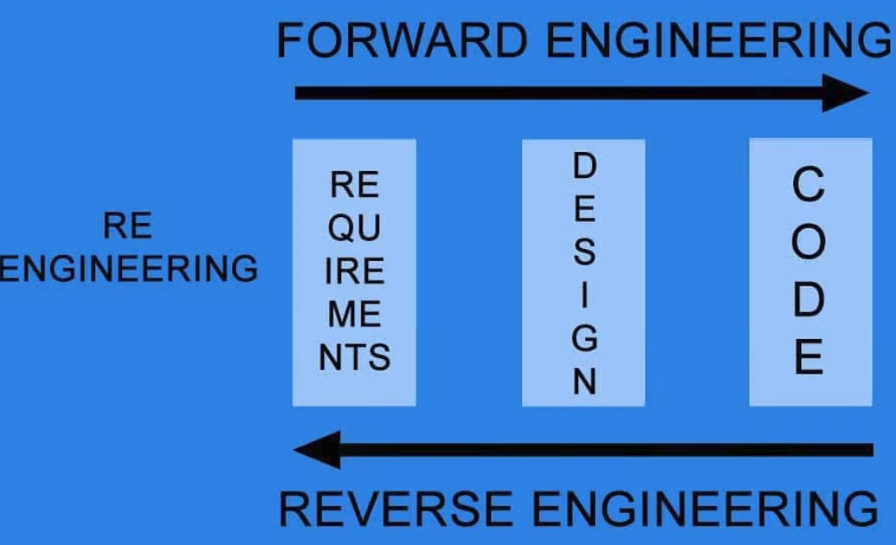
\includegraphics[width=0.5\linewidth]{Chapitre1/figures/reverse.png}
  \caption{Reverse engineering procedure (source: \url{https://t2informatik.de/en/smartpedia/reverse-engineering/})}
  \label{malicious}
\end{figure}

Fault Injection Attacks (FIA) \cite{hsueh1997fault} involve deliberately inducing faults into the hardware with the goal of altering its normal behavior(as Figure \ref{fault injection}). These faults can be transient or permanent and may be introduced through methods such as voltage glitches, clock disturbances, electromagnetic pulses, laser beams, or thermal stress. By causing errors in computation or control flow, attackers can bypass security checks, extract secret information, or compromise critical functions. FIA represents a powerful attack vector, particularly because it operates at the boundary between physical disturbance and software response.

\begin{figure}[t!]
  \centering
  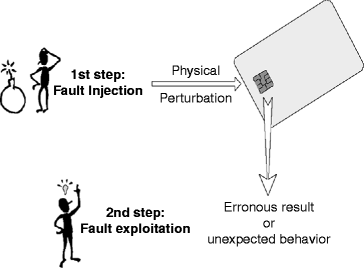
\includegraphics[width=0.5\linewidth]{Chapitre1/figures/fault.png}
  \caption{Fault injection procedure (source: \url{https://link.springer.com/rwe/10.1007/978-1-4419-5906-5_505})}
  \label{fault injection}
\end{figure}

Side-Channel Attacks (SCA) \cite{kelsey1998side} as Figure\ref{side channel attack} exploit information that leaks unintentionally during the normal operation of a device. These leaks can manifest as variations in power consumption, electromagnetic emissions, timing behavior, or even acoustic signals. By observing and analyzing these physical side effects, attackers can infer secret data such as cryptographic keys or internal program states. Unlike fault injection, SCA does not aim to alter system behavior, but rather to passively observe it with high precision.

\begin{figure}[t!]
  \centering
  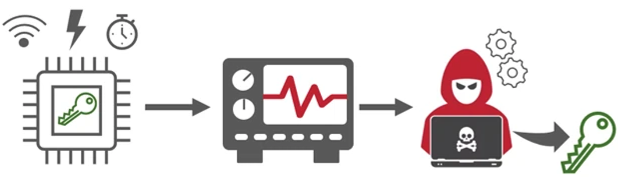
\includegraphics[width=0.5\linewidth]{Chapitre1/figures/sca.png}
  \caption{Side-Channel Attacks procedure (source: \url{https://semiengineering.com/secure-your-soc-from-side-channel-attacks-with-adaptable-security/})}
  \label{side channel attack}
\end{figure}

Hardware Trojan Insertion \cite{chakraborty2009hardware} as Figure \ref{hardware trojan} refers to the deliberate embedding of malicious logic within a hardware design. This can occur during design, fabrication, or post-fabrication stages, often without detection. Hardware Trojans may remain dormant until triggered by specific conditions, at which point they can leak information, degrade performance, or disable functionality. Their stealthy nature and integration within legitimate hardware make detection and prevention especially challenging.

\begin{figure}[t!]
  \centering
  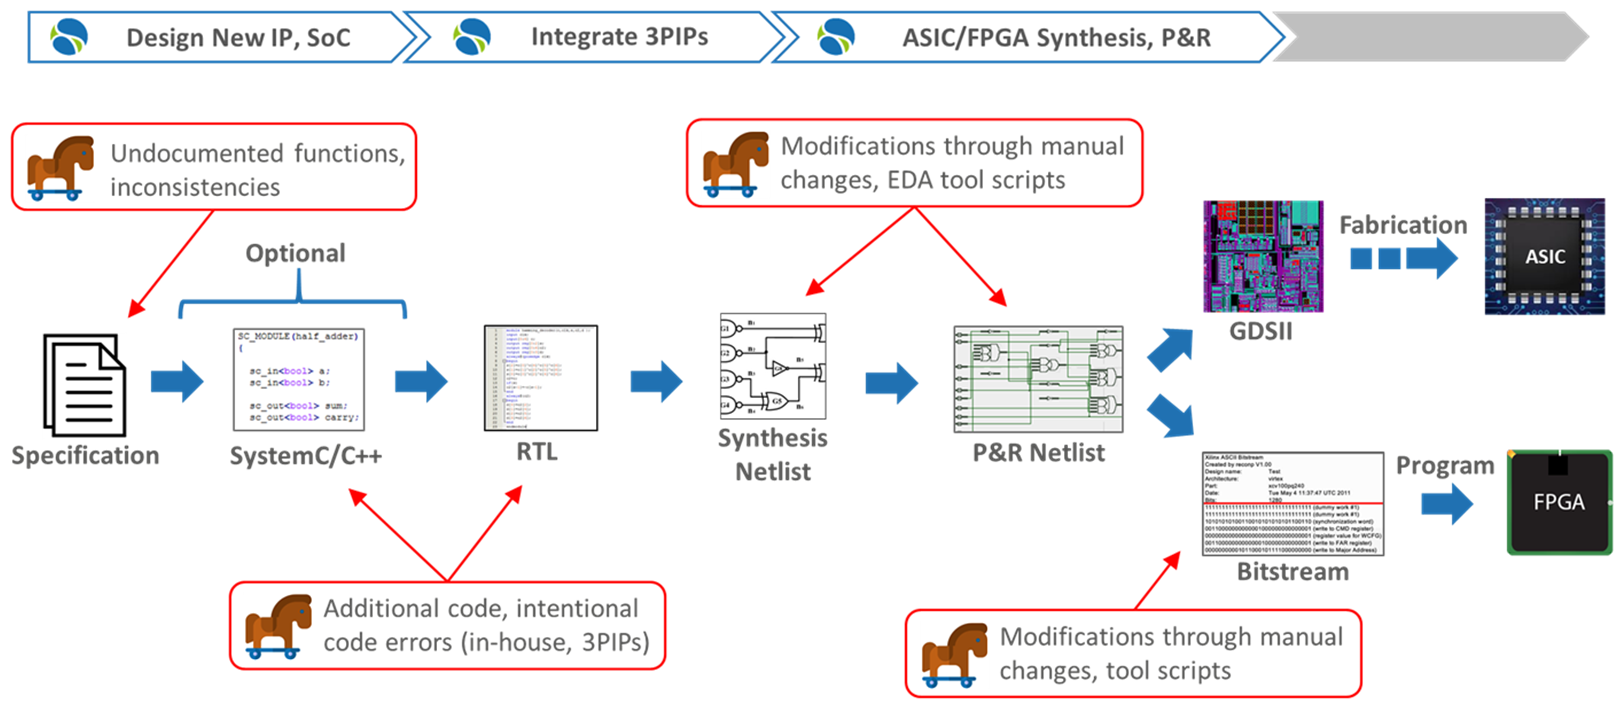
\includegraphics[width=0.5\linewidth]{Chapitre1/figures/hardware trojan.png}
  \caption{Hardware Trojan Insertion procedure (source: \url{https://semiengineering.com/hardware-trojans-and-the-problem-of-trust-in-integrated-circuits/})}
  \label{hardware trojan}
\end{figure}

\subsection{Fault Injection methods}

Clock fault injection (Figure \ref{clock fault}) can be achieved through several mechanisms, including manipulating the clock period, introducing voltage disturbances, or intentionally reducing the power supply. In the case of clock manipulation, reducing the clock period may result in insufficient setup time for certain signal paths, causing data to arrive at flip-flops too late relative to the clock edge. This misalignment can lead to erroneous values being captured. An early implementation of this technique was presented by Agoyan et al. \cite{agoyan2010clocks}, who targeted an AES encryption core implemented on an FPGA with a delay-locked loop (DLL)-based clocking system. Similar results were reported in \cite{selmke2019peak}, where externally induced glitches affected the clock signal of an ARM-based microcontroller, even though the internal system clock was derived from a phase-locked loop (PLL), illustrating the vulnerability of PLL-based systems to external perturbations.

\begin{figure}[t!]
  \centering
  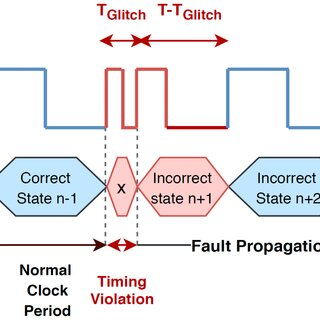
\includegraphics[width=0.5\linewidth]{Chapitre1/figures/clock fault.jpg}
  \caption{Clock fault principle (source: \url{https://www.researchgate.net/figure/Representation-of-clock-glitch-and-fault-injection-17_fig4_343027498})}
  \label{clock fault}
\end{figure}

Voltage-based fault injection methods (Figure \ref{voltage fault}) exploit the delay characteristics of CMOS circuits under reduced supply conditions. By introducing brief voltage drops or operating the device under nominal voltage thresholds, attackers can increase the signal propagation delay within the combinational logic. This delay may prevent correct evaluation before the next clock edge, thereby injecting computation faults. Selmane et al. \cite{selmane2008practical} demonstrated this principle in a practical attack scenario, where underpowering a smart card executing AES operations resulted in faulty outputs. Later investigations, such as the one conducted by Zussa et al. \cite{zussa2013power}, examined the impact of negative voltage pulses on FPGA implementations. Their findings indicated that the observable fault patterns induced by power glitches closely resemble those caused by clock manipulation, suggesting a convergence in their physical effects.

\begin{figure}[t!]
  \centering
  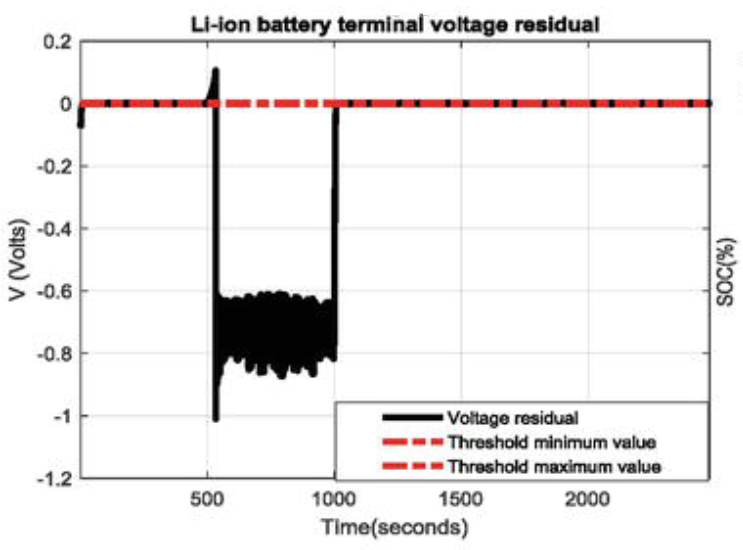
\includegraphics[width=0.5\linewidth]{Chapitre1/figures/voltage.png}
  \caption{Voltage fault waveform (source: \url{https://www.intechopen.com/chapters/74031})}
  \label{voltage fault}
\end{figure}

Electromagnetic (EM) (Figure \ref{electromagnetic fault}) interference represents another class of fault injection, relying on the alteration of timing relationships within the circuit \cite{trouchkine2021electromagnetic} ~\cite{trouchkine2021fault}. When exposed to strong EM fields, the synchronization between clock signals and data lines can be disturbed. As a result, bits stored in memory cells or registers may be erroneously set or reset. This form of attack was pioneered by Quisquater et al. ~\cite{quisquater2002eddy}, who demonstrated that applying electromagnetic perturbations to various memory technologies could induce fault conditions in a contactless and localized manner. In this paper~\cite{sass2023oops}, they present \textmu-Glitch, the first Voltage Fault Injection (VFI) platform which is capable of injecting multiple, coordinated voltage faults into a target device, requiring only a single trigger signal. Their evaluation revealed that \textmu-Glitch can successfully inject four consecutive faults within an average time of one day.

\begin{figure}[t!]
  \centering
  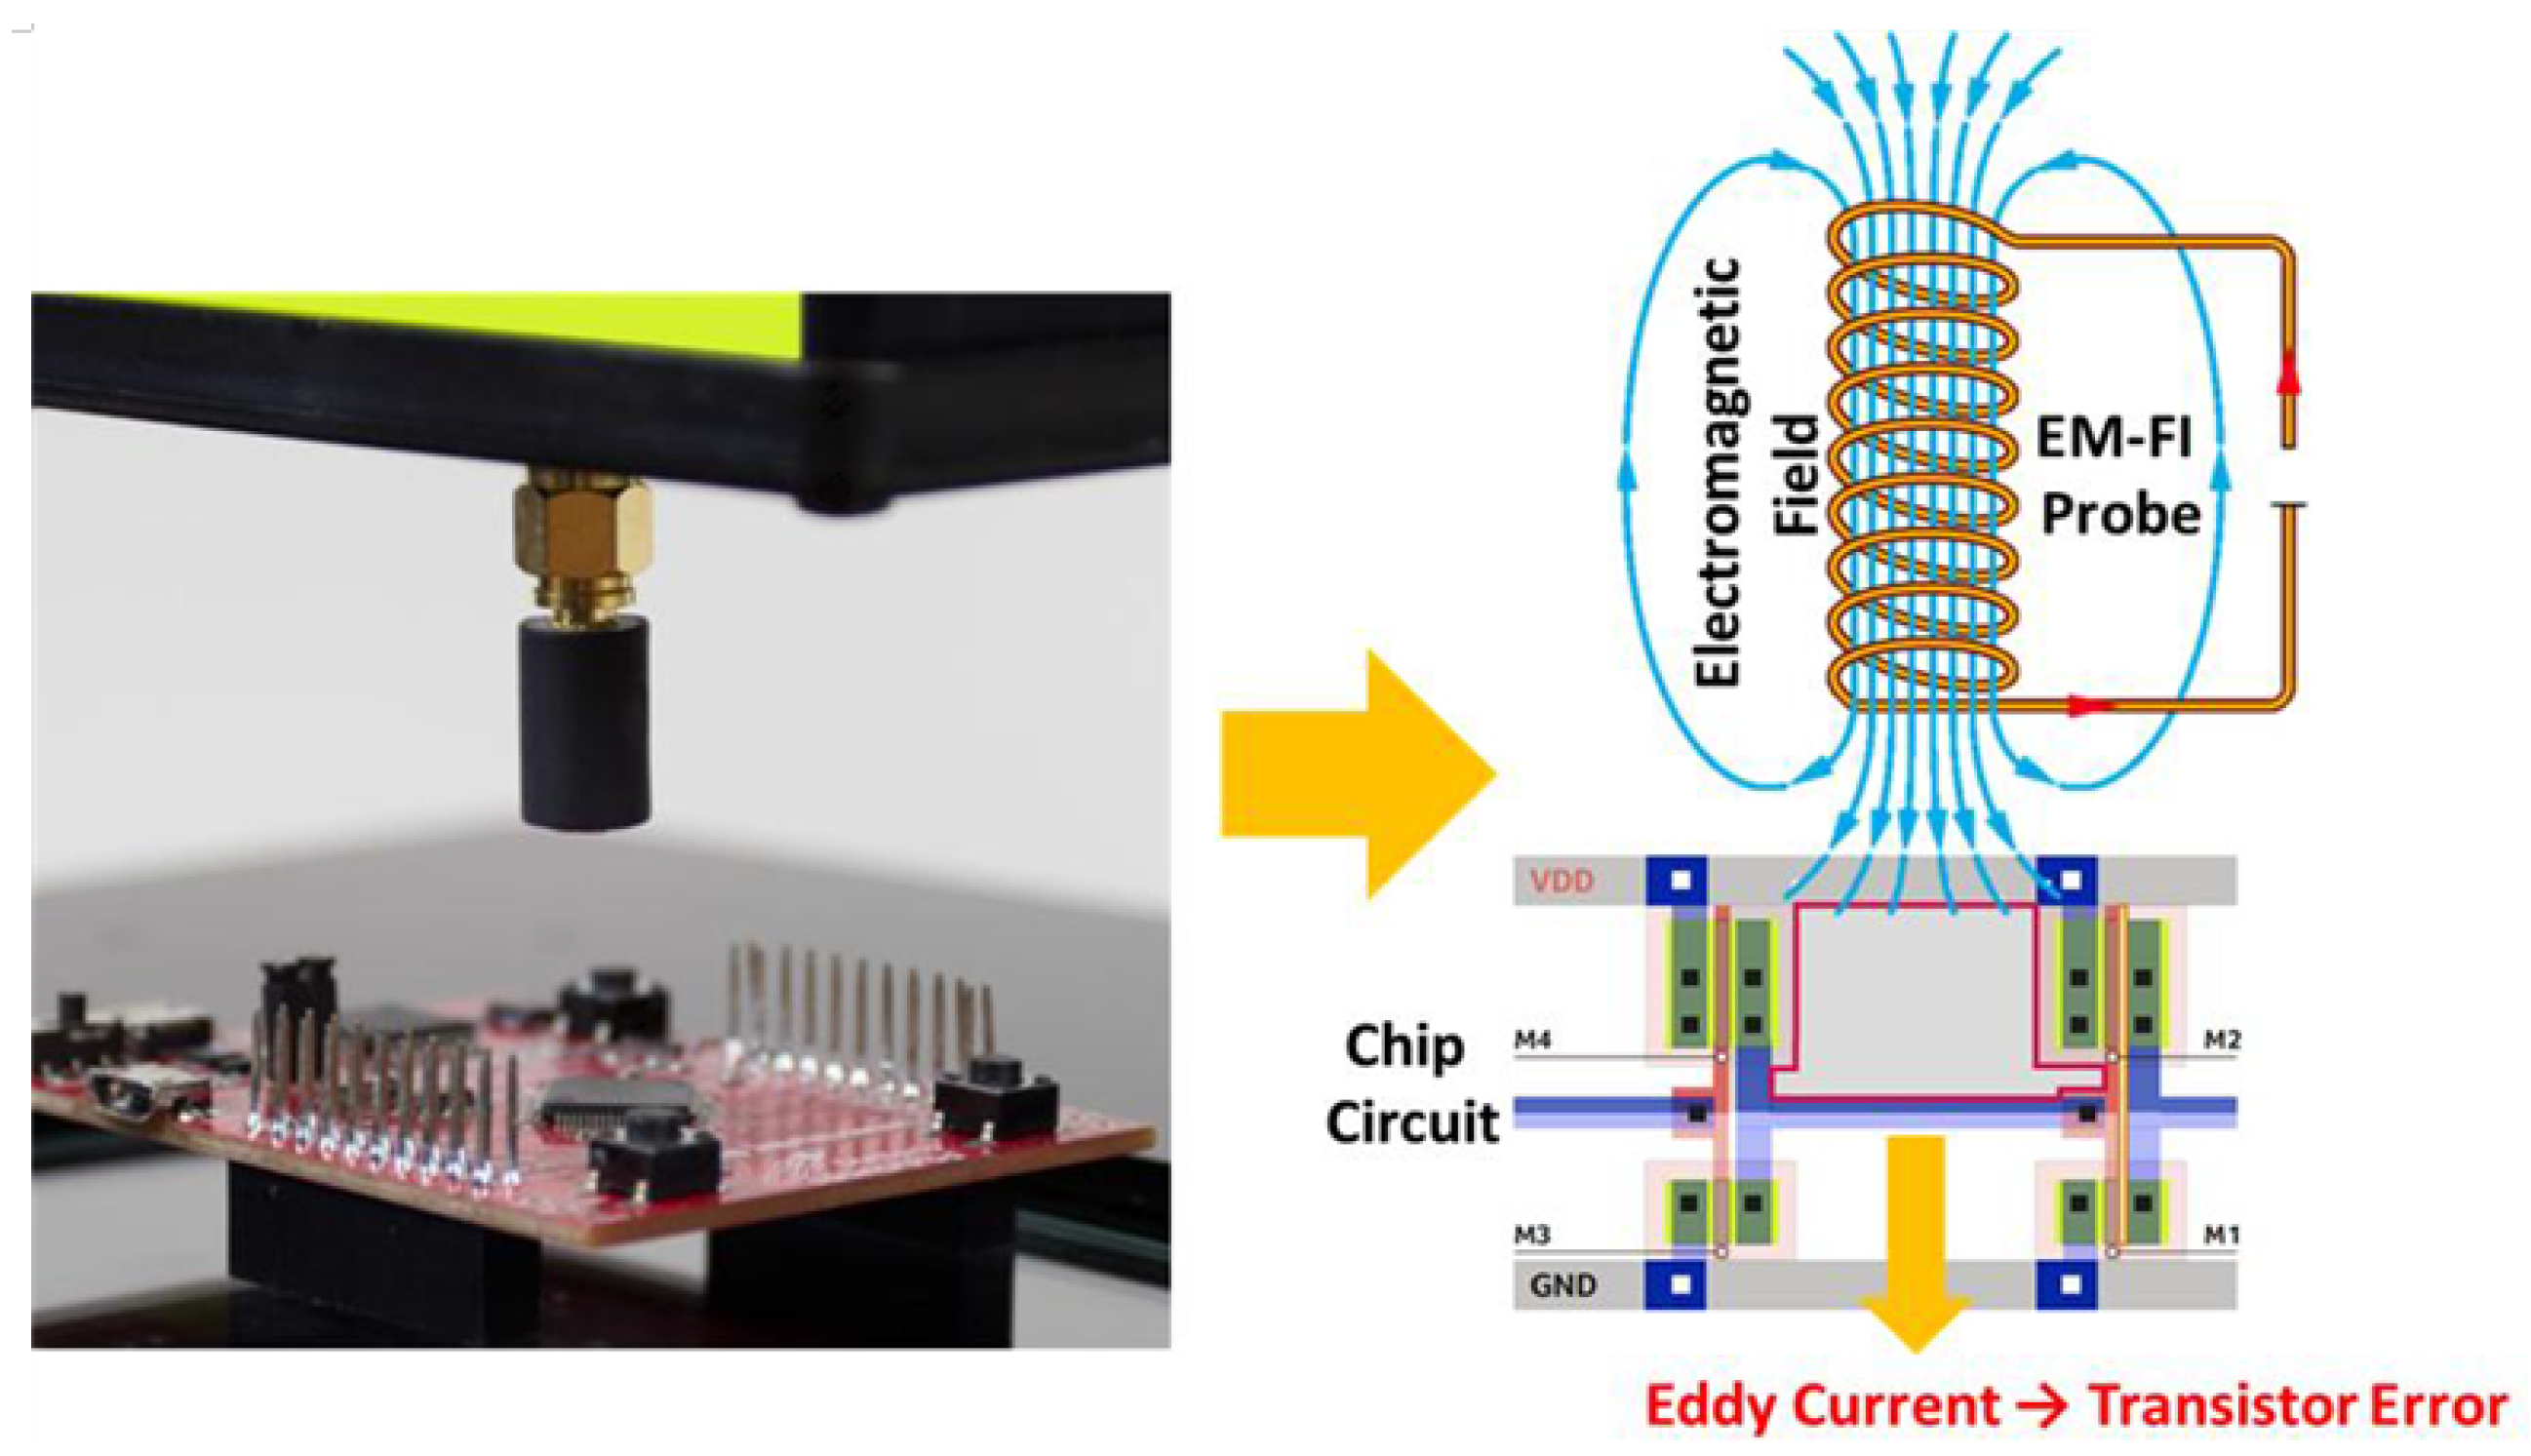
\includegraphics[width=0.5\linewidth]{Chapitre1/figures/em.png}
  \caption{Electromagnetic fault principle (source: \url{https://www.researchgate.net/figure/Representation-of-clock-glitch-and-fault-injection-17_fig4_343027498})}
  \label{electromagnetic fault}
\end{figure}

Optical injection techniques (Figure \ref{optical fault}) provide finer spatial resolution. The first optical fault injection attack was proposed by Skorobogatov and Anderson~\cite{skorobogatov2003optical}, where they utilized a photographic flash to disturb SRAM cells in microcontrollers. This approach exploits the light sensitivity of semiconductor materials, where photons generate transient charge carriers that alter the state of logic gates or memory elements. More advanced implementations later used focused laser beams to achieve precise control over the affected region, allowing faults to be targeted at specific registers or datapaths.

\begin{figure}[t!]
  \centering
  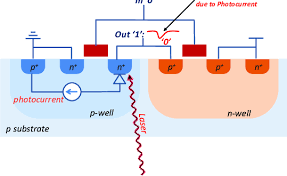
\includegraphics[width=0.5\linewidth]{Chapitre1/figures/laser.png}
  \caption{Laser fault attack on CMOS (source: \url{https://www.researchgate.net/figure/Laser-Fault-Injection-LFI-mechanism-in-the-case-of-a-simple-CMOS-inverter_fig1_376090023})}
  \label{optical fault}
\end{figure}

In addition to the techniques mentioned above, fault injection through body biasing and X-ray irradiation has also been explored. Body biasing alters the threshold voltage of transistors by adjusting the substrate potential, thereby increasing the susceptibility of certain regions to timing violations. This was demonstrated in the work of Tobich et al. \cite{tobich2012yet} and later refined by O'Flynn et al. \cite{o2021low}. On the other hand, nanofocused X-ray beams have been proposed as a means to disturb circuit behavior at the atomic scale. Anceau et al.~\cite{anceau2017nanofocused} investigated the feasibility of this method, showing that localized exposure can lead to significant disruption in device functionality, although the technique currently remains within the domain of laboratory-scale experiments.

\subsection{Fault Injection Hierarchy}
Fault injection attacks can be understood across several abstraction layers of a computing system, from high-level software instructions down to the physical behavior of transistors. This hierarchical view is essential for understanding the range of possible effects a fault may induce, as well as for designing appropriate countermeasures.

At the \textit{instruction level}, attackers aim to corrupt the program’s control flow or logic by targeting the encoding of instructions. One common strategy is instruction skipping, where the execution of one or more instructions is prevented, effectively bypassing conditional checks or security validations~\cite{alshaer2022cross, dehbaoui2013electromagnetic}. In more complex scenarios, attackers have demonstrated the ability to skip multiple consecutive instructions~\cite{riviere2015high, nashimoto2017buffer}, or to cause a single instruction to be executed repeatedly or replaced with a different operation~\cite{khuat2021laser, alshaer2022variable, balasch2011depth, timmers2016controlling}. These manipulations alter the intended meaning of the program without modifying the binary, which makes them difficult to detect through static analysis alone.

At the \textit{micro-architectural level}, faults interact with internal processor components such as pipeline stages, register files, and cache hierarchies. These attacks disrupt implicit hardware assumptions about timing, resource arbitration, or speculative execution. For instance, faults can interfere with instruction decoding or pipeline forwarding logic, leading to unintended execution paths or stale data propagation~\cite{Tollec2022exploration}. Micro-architectural-level effects are often more difficult to model, as they depend on the specific implementation of the processor, including undocumented behaviors or vendor-specific optimizations.

At the \textit{circuit level}, attackers target the electrical properties of the digital logic itself. By manipulating signal propagation delays or altering the threshold voltage of transistors, an attacker may induce incorrect switching behavior in gates or flip-flops. This could result in bit flips, stuck-at faults, or randomization of signal values. Depending on the fault model, the effect may corrupt a single bit, a byte, or even entire registers or memory words—potentially affecting security-critical variables such as cryptographic keys or control flags~\cite{barenghi2012fault, marc2012fault}. Faults at this level can be induced using techniques such as voltage glitches, electromagnetic pulses, or laser irradiation, and typically require precise spatial and temporal alignment to be effective.

To comprehensively evaluate system resilience, it is important to understand how faults at lower levels of the hierarchy propagate to higher levels. For example, a transient fault at the transistor level may manifest as a corrupted instruction in the pipeline, which in turn may result in a logic bypass or privilege escalation at the software level. Therefore, defense strategies must be designed with cross-layer awareness, accounting for both the physical origin of faults and their logical consequences across abstraction boundaries.

\subsection{Fault Injection Countermeasure}
Despite the fact that multiple architectural layers remain vulnerable to fault injection attacks, a variety of defensive techniques have been developed to enhance system robustness. These countermeasures aim either to detect, withstand, or obscure the effects of injected faults, and are typically implemented at different abstraction levels. While none of these methods offer absolute protection, their combined application can significantly increase the difficulty of mounting a successful attack.

A first class of countermeasures focuses on \textit{fault detection and correction}, where the primary objective is to identify the occurrence of faults and respond appropriately. Most of these strategies rely on introducing some form of redundancy. For instance, hardware-level duplication—known as modular redundancy—executes the same operation in parallel on multiple instances of the same logic, with consistency checks performed on the outputs~\cite{dutertre2011review}. Alternatively, \textit{time redundancy} involves re-executing computations at different time intervals and comparing results~\cite{manssour2022processor}. At the data level, \textit{information redundancy} techniques, such as parity bits or error detection codes, are used to encode and verify the integrity of sensitive variables~\cite{yuce2016fame}~\cite{elbaz2009hardware}. However, these approaches can be circumvented if the injected fault affects multiple redundant elements simultaneously or occurs in such a way that errors cancel out across the comparison logic.

In parallel, \textit{isolation-based defenses} have proven effective in limiting the adversary's ability to physically interact with or influence the critical regions of a chip. One practical measure is the use of physical shielding, which encloses vulnerable zones of the device with protective layers to prevent optical, electromagnetic, or mechanical access~\cite{avital2024enhancing}. Another complementary technique involves signal \textit{filtering}, where components such as integrated voltage regulators or passive filters are inserted between external interfaces and the internal circuit to attenuate the impact of voltage glitches or electromagnetic transients~\cite{fanjas2022combined}. These forms of isolation are especially relevant when combined with tamper-evident packaging or sensor-triggered response logic~\cite{qi2016design}.

To further complicate the timing precision required for fault injection, many implementations incorporate \textit{desynchronization techniques}, sometimes referred to as temporal or architectural randomization. As for the software countermeasure, the core idea is to introduce unpredictability into the execution flow, making it more difficult for attackers to align their fault attempts with specific instruction boundaries or computation phases. This can be achieved by using non-deterministic internal clock sources, random delays, instruction shuffling, or injecting dummy operations~\cite{patrick2017lightweight, wang2016against}. While these techniques can greatly reduce fault success rates under brute-force conditions, more sophisticated attacks have emerged that exploit residual patterns. Notably, approaches such as Fault Intensity Map Analysis (FIMA) \cite{ramezanpour2019fima} and Statistical Ineffective Fault Attacks (SIFA) \cite{dobraunig2018statistical} use statistical modeling and spatial fault profiling to recover fault injection parameters, even in randomized environments.

Collectively, these countermeasures illustrate the ongoing arms race between fault injection techniques and defensive engineering. A robust defense strategy requires not only the layering of these countermeasures, but also a clear understanding of the attacker model, fault injection capabilities, and the system’s operational context.

\section{Studies Combining Hardware-Software Attacks}
In modern embedded systems, the boundary between hardware and software security is increasingly blurred. While hardware and software attacks are often studied separately, a growing body of research has demonstrated that combined hardware-software attack strategies—which exploit the interplay between physical-layer vulnerabilities and software-level logic—can significantly amplify the effectiveness and stealth of an attack. These hybrid techniques represent a sophisticated threat model that is particularly relevant in the context of complex SoC designs, where hardware, firmware, and application code interact tightly and often rely on shared resources and assumptions.

At their core, combined attacks exploit the physical ability to induce faults or extract side-channel information, while leveraging software logic or architectural knowledge to guide, refine, or interpret the results of such manipulation. This technique is particularly powerful in scenarios such as instruction skipping, faulting condition checks, or bypassing cryptographic authentication.

One of the most well-known examples of this combination is the fault attack on software-controlled cryptographic operations, where physical disturbances are introduced at precisely timed execution stages \cite{buhren2021one}. For instance, fault injection may be used to corrupt a register holding an intermediate value of an AES computation, and then a software routine may capture the faulty output and perform differential analysis to recover the secret key. Such attacks—e.g., DFA (Differential Fault Analysis) \cite{biham1997differential} —demonstrate how precise hardware faults can be exploited through structured software-level observation.

Another common form of combined attack occurs in control-flow manipulation ~\cite{carlini2015control} ~\cite{bouffard2011combined}, where the attacker induces faults in the instruction decoding or branching logic of the processor, causing the software to skip authentication checks, execute unintended code paths, or return prematurely from protected routines. These faults, though induced physically, have purely software-visible consequences, and often remain undetected without explicit control-flow integrity mechanisms.

Advanced combined attacks have also emerged in the form of hardware Trojan ~\cite{chakraborty2009hardware} triggers activated by software behavior. In such cases, a malicious circuit embedded within the chip may remain dormant until specific software conditions—such as a unique sequence of instructions or memory access patterns—are met. This attack model reverses the typical direction of influence, demonstrating that software itself can serve as a vector for activating hidden hardware-level threats.

In addition, the recent rise of micro-architectural attacks \cite{8740838}—such as Spectre, Meltdown, and their variants—has further demonstrated the inseparability of hardware and software in the security domain. These attacks exploit hardware features like speculative execution, branch prediction, or cache coherence, but rely on carefully constructed software to leak information via side-channels. Such attacks bypass traditional privilege boundaries without requiring direct code injection or physical access, underlining the danger of ignoring the interaction between hardware design choices and software observability.

In summary, combined hardware-software attacks represent a significant escalation in adversarial capability. By simultaneously leveraging physical fault injection or side-channel techniques with logical exploitation through software, attackers can compromise systems that would otherwise be resistant to purely physical or purely logical attacks alone. Defending against such threats requires an integrated security approach that considers not just individual layers, but the interaction between them—emphasizing the need for co-designed, cross-layer countermeasures in secure system development.

\section{Communication architecture}
In modern System-on-Chip (SoC) designs, the communication architecture plays a critical role in coordinating data transfer and control signal exchange among computational cores, memory units, and peripheral components. As the complexity and scale of SoCs continue to grow, selecting an appropriate communication architecture becomes essential for ensuring performance, scalability, and reliability.

Historically, bus-based architectures have served as the dominant communication model in SoC development. These systems rely on a shared communication medium, where multiple modules transmit and receive data through a centralized interconnect. Buses offer simplicity in design and are well-suited for small to medium-scale SoCs with a limited number of functional blocks. However, as the number of cores and modules increases, bus architectures encounter fundamental limitations, including bandwidth contention, arbitration latency, and scalability bottlenecks.

Buses are inherently susceptible to various forms of attacks. For instance, in \cite{rodrigues2024busted}, the authors present a novel side-channel attack that leverages unintended side effects of the microcontroller bus interconnect arbitration logic to circumvent memory protection mechanisms. Unlike their approach, which exploits side-channel leakage, our work focuses on actively injecting faults into the bus to compromise its behavior. In another study \cite{5979407}, the authors concentrate on an external-bus fault injection system designed to meet PHM verification test requirements. They developed and validated a fault injector targeting the RS-485 bus and constructed a simulated experimental environment to assess its effectiveness. While their work presents fault injection results, it is limited in scope—relying on a single fault model and lacking an in-depth analysis of how the faults propagate and affect bus functionality. In contrast, our research explores a broader range of fault models and offers a more comprehensive evaluation of fault impacts on bus behavior.

To address these limitations, researchers and industry designers have progressively adopted Network-on-Chip (NoC) architectures. A NoC replaces the shared medium with a structured, packet-switched interconnection network composed of routers and point-to-point links. This decentralized topology facilitates parallel communication paths, allowing simultaneous data transfers across different modules. As a result, NoC architectures offer significant improvements in bandwidth utilization, modularity, and system scalability, particularly in multicore and manycore designs.

Similarly, fault attacks pose significant threats to Network-on-Chip (NoC) architectures. One study evaluates the fault tolerance of NoC routers using a simulation-based approach to assess their resilience under fault conditions. In \cite{5196018}, the authors employ multiple fault models—similar to our methodology—but their analysis lacks the depth and detail presented in our evaluation. Another work \cite{8704559} introduces a hybrid fault injection approach combining both FPGA-based and layout-level techniques. While this paper provides a comprehensive analysis of the fault injection results, it does not propose any concrete countermeasures, in contrast to our work, which addresses both evaluation and mitigation strategies.

From a high-level perspective, both bus and NoC architectures are instantiations of communication backbones that govern how information flows within a chip. The key distinction lies in their topology and traffic handling capabilities—while buses favor centralized simplicity, NoCs embrace distributed flexibility.

In the subsequent section, we delve into bus-based protocols, including Wishbone, AXI-Lite, and AXI, which represent widely used standards in both academic and industrial SoC platforms. Following that, a detailed examination of Network-on-Chip architectures is presented, emphasizing their relevance in fault-tolerant and high-performance embedded systems.

\section{Objective}
The overarching objective of this research is to strengthen the security and resilience of embedded system-on-chip (SoC) architectures against fault injection attacks targeting on-chip communication buses. These buses, such as Wishbone\cite{wishbone_spec}, AXI-Lite\cite{axi_lite_spec}, and AXI\cite{axi_spec}, are widely deployed in modern embedded systems due to their modularity and reusability. However, their standardized structure and predictable communication behavior make them attractive targets for attackers aiming to disrupt or manipulate system functionality through physical or semi-invasive fault injection methods. While prior studies have illustrated the feasibility of bus-level attacks, particularly focusing on individual protocols, a comprehensive analysis across multiple bus architectures remains lacking.

To address this gap, the first goal of this study is to perform an in-depth analysis of the Wishbone bus architecture as a representative open-source interconnect standard. By systematically examining the timing behavior, handshake mechanisms, and signal integrity constraints of the bus, the research identifies key vulnerabilities that could be exploited by adversaries to compromise data integrity, control flow, or address resolution. This architectural-level understanding also enables generalization to other bus types, such as AXI-Lite and AXI, where similar principles apply but may manifest differently due to protocol complexity and pipeline structures.

Building upon this vulnerability analysis, the research proceeds to explore and evaluate existing countermeasures, both hardware-based and software-based, that aim to protect system buses against such threats. Through critical comparison, it is shown that software-only protections, such as instruction redundancy or control flow checking, are often insufficient when attacks target the hardware transmission layers directly. These limitations motivate the design of a new hardware-level defense mechanism that integrates directly into the communication bus architecture. The countermeasure proposed in this work is tailored to detect and mitigate a wide range of fault injection scenarios while maintaining low overhead and compatibility with existing system designs.

Furthermore, the effectiveness of the proposed solution is demonstrated through experimental evaluation and side-by-side comparison with alternative approaches. By conducting fault injection campaigns across multiple bus protocols and measuring the resilience of different protection schemes, the research offers empirical evidence of the robustness and practicality of the proposed hardware defense. The study ultimately aims to bridge the gap between theoretical vulnerability models and deployable protection strategies, contributing to the development of more secure SoC platforms in adversarial environments.

\section{Conclusion}
This chapter provided a comprehensive overview of system-level attacks with a focus on their classification, technical mechanisms, hierarchical impact, and corresponding countermeasures. By establishing a clear definition of "attack" as any deliberate action that aims to degrade the security level of an embedded electronic system, we structured the discussion around two primary dimensions: hardware-based and software-based attacks.

Hardware attacks were introduced as physical or semi-invasive actions that exploit the electrical or structural properties of a system. Various forms were discussed, including reverse engineering, fault injection, side-channel analysis, and hardware Trojan insertion, each characterized by its mode of access and impact on system behavior. The discussion on fault injection was further detailed through its history, methods of realization, and the abstraction levels it can affect—from individual logic gates to high-level control logic—highlighting its growing relevance in real-world threat models.

Software attacks, on the other hand, were examined from the perspective of logical exploitation, code manipulation, and privilege escalation. These attacks often interact with the execution environment, targeting software-level assumptions through vulnerabilities in code structure, memory handling, or control flow. As with hardware threats, software attacks were analyzed across different layers of abstraction, from instruction-level manipulation to micro-architectural interference and logic corruption at the circuit level.

A key aspect of this chapter was the hierarchical analysis of attacks, which clarified how vulnerabilities can propagate from low-level physical phenomena to observable software malfunctions. Understanding this multi-layer relationship is critical in the design of effective defenses. Correspondingly, the chapter presented a survey of countermeasure strategies, ranging from redundancy and detection logic to isolation and desynchronization techniques. These solutions were categorized based on their level of implementation and their defensive focus, revealing the strengths and limitations of each approach.

Together, the materials presented in this chapter form the foundation for the technical analyses in the following chapters. The detailed classification and modeling of attacks provide a structured lens through which specific vulnerabilities in SoC interconnects—particularly communication buses—can be examined. To further ground the theoretical concepts discussed in this chapter, the following chapter details the practical environment in which fault injection experiments are conducted. It outlines the SoC architecture constructed with LiteX, elaborates on the bus systems under investigation, defines the fault models applied, and presents the experimental assumptions and benchmarks used to evaluate the impact and detectability of system-level attacks.

\clearemptydoublepage
\chapter{Experiment setup}
Building upon the theoretical framework established in the previous chapter, this chapter introduces the experimental environment used to validate and explore fault-based attacks on SoC interconnects. The structured classification and modeling of vulnerabilities serve as a foundation for the practical investigation that follows. Here, we present the concrete system setup developed to test communication bus security under controlled fault conditions. Specifically, we describe the SoC architecture implemented using the LiteX framework, explain the configuration of the target bus protocols, and define the fault models and attacker assumptions adopted in our study. In addition, we outline the benchmarks and evaluation criteria used to assess the system’s resilience and the effectiveness of potential countermeasures.

\section{Construction SoC}
In order to systematically study fault injection attacks targeting on-chip buses, it is necessary to construct custom SoC platforms where the internal architecture—including interconnects, memory hierarchies, and processor interfaces—can be precisely controlled. This level of flexibility is difficult to achieve using vendor-locked design environments or pre-built SoC platforms, which often lack transparency and configurability at the system level.

To meet these requirements, we chose the LiteX framework. LiteX provides fine-grained control over system configuration, allowing us to tailor bus protocols, memory layouts, and peripheral mappings to suit specific attack scenarios. Moreover, its compatibility with a wide range of FPGA boards ensures that experiments can be reproduced across different hardware targets without extensive redesign. The framework also supports both simulation and hardware deployment from a unified design space, enabling efficient prototyping and testing of attack models.

In the following section, we provide a detailed overview of the LiteX architecture and explain how its features support our experimental goals.
\subsection{LiteX}
The increasing availability of open-source hardware development tools has significantly improved the accessibility and reproducibility of system-on-chip (SoC) research. Among these tools, LiteX (Figure \ref{litex}) has emerged as a versatile and powerful SoC builder framework, designed to streamline the process of constructing FPGA-based systems. Developed by the EnjoyDigital community, LiteX leverages the flexibility of Python and provides a modular and extensible platform for designing, simulating, and deploying digital systems with a high degree of customization.

\begin{figure}[t!]
  \centering
  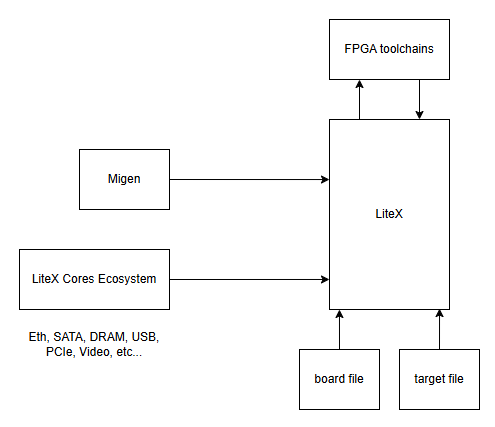
\includegraphics[width=0.5\linewidth]{Chapitre2/figures/litex.png}
  \caption{Component of LiteX framework}
  \label{litex}
\end{figure}

LiteX \cite{litex} provides a comprehensive set of pre-integrated building blocks essential for SoC development. This includes support for common bus protocols and streaming interfaces—such as Wishbone, AXI, and Avalon-ST—along with their corresponding interconnect infrastructure. Core components such as RAM, ROM, UARTs, timers, and JTAG interfaces are readily available, while more sophisticated IP cores—including LiteDRAM, LitePCIe, LiteEth, and LiteSATA—are seamlessly integrated into the ecosystem. The framework supports a variety of CPU architectures and instruction sets, such as RISC-V (e.g., VexRiscv), OpenRISC, LM32, and even x86 (via PCIe integration), enabling both lightweight microcontroller-class SoCs and more complex, Linux-capable multicore systems.

One of the key enablers behind LiteX's flexibility is its foundation in Migen (short for Milkymist generator), a Python-based hardware description library designed to overcome the inefficiencies and limitations of traditional HDLs like Verilog and VHDL. Migen replaces the event-driven model with explicit combinatorial and synchronous constructs, simplifies arithmetic semantics to better reflect mathematical expectations, and, most importantly, allows for procedural generation of logic using standard Python features. This metaprogramming capability empowers developers to write reusable, parameterized, and highly structured hardware designs by leveraging object-oriented patterns, operator overloading, Python generators, and more.

Through the combination of Migen and LiteX, designers benefit from an ecosystem that supports multiple languages (including VHDL, Verilog, SpinalHDL, and nMigen), offers built-in simulation via Verilator for fast and accurate modeling, and includes powerful debugging tools such as Litescope and software bridges for real-time analysis. Furthermore, LiteX supports multiple backend flows, including both open-source and vendor-specific toolchains, enhancing portability and deployment flexibility.

Despite these capabilities, LiteX does not explicitly address security concerns in its architectural design or development workflows. Its primary focus remains on flexibility, modularity, and ease of integration across diverse hardware platforms. This lack of built-in security mechanisms—such as privilege enforcement, fault injection resistance, or hardware isolation—makes it a particularly interesting target for security research. Given its increasing adoption in research and prototyping contexts, analyzing LiteX from a security perspective is not only timely but essential. Investigating its behavior under adversarial conditions can help identify architectural gaps and motivate the development of lightweight, security-enhanced extensions suitable for resource-constrained environments.

In this research, we adopt LiteX as the foundation for constructing various SoC instances that serve as testbeds for our fault injection experiments. The platform enables the controlled configuration of interconnects (e.g., Wishbone vs AXI-Lite), memory subsystems, and processor types, facilitating detailed comparisons across different architectural choices. The ability to instrument hardware, modify firmware, and run cycle-accurate simulations within a unified development environment makes LiteX particularly well-suited for studying software-assisted fault attacks. Notably, complex SoCs—such as a multicore Linux-capable system based on VexRiscv-SMP, LiteDRAM, and LiteSATA—can be assembled, tested, and deployed using LiteX, even on cost-effective FPGA platforms.

\subsection{SoC configuration}
As we talk before, we designed a highly customizable and transparent system-on-chip (SoC) platform to support controlled experimentation of fault injection attacks targeting interconnect-level vulnerabilities. This platform was implemented using the LiteX framework, which enables fine-grained architectural control and streamlined deployment on FPGA hardware. Each component of the SoC—from the processor core to the interconnects and memory subsystem—was carefully selected to facilitate precise observation, fault reproducibility, and architectural flexibility across experimental scenarios.

At the heart of the system is the VexRiscv soft-core CPU, an open-source implementation of the RISC-V instruction set. We selected RISC-V for its minimalistic and modular architecture, which simplifies reasoning about instruction-level behavior during fault injection. The open specification of RISC-V provides complete transparency over instruction decoding, execution semantics, and control paths—properties essential for correlating fault effects with specific hardware events. VexRiscv’s configurability, small footprint, and close integration with the LiteX ecosystem make it ideal for deploying on resource-constrained FPGA platforms while maintaining the option to scale up with more advanced features. Furthermore, VexRiscv’s support for real-time debugging and visibility into register-level state significantly aids in fault localization.

To analyze the impact of bus-level faults in varied contexts, we designed the SoC to support three major interconnect protocols: Wishbone, AXI, and AXI-Lite. These buses differ in complexity and transaction semantics, offering diverse opportunities for observing different classes of fault behavior. Wishbone, as a synchronous and minimal protocol, is easy to analyze and useful for capturing fundamental fault patterns. In contrast, AXI introduces advanced features such as out-of-order execution, burst transfers, and independent read/write channels, thereby increasing the range and subtlety of observable vulnerabilities. AXI-Lite, a subset of AXI without burst or outstanding transaction support, serves as a middle ground—maintaining AMBA compatibility while retaining relatively simple timing. By keeping the rest of the SoC architecture constant, we can isolate the impact of the bus protocol itself when assessing system-level fault behavior.

The memory architecture of the SoC includes four primary regions: ROM, SRAM, CSR (Control and Status Registers), and an additional MAIN\_RAM block. The ROM is used to store program binaries and is loaded at synthesis time. To ensure maximal control over program behavior, all software is compiled into unoptimized assembly using the RISC-V GCC toolchain with -O0 optimization level. This prevents the compiler from reordering instructions or introducing artifacts that could obscure fault propagation paths. By using hand-tuned or compiler-generated low-level code, we achieve consistency across test cases and precise mapping between source and hardware behavior.

SRAM is used as the main runtime memory for variables, stack, and temporary data. The CSR region is memory-mapped and provides access to internal system signals such as timers, bus status, and control flags. These are particularly useful for monitoring injected fault effects from within the program itself. To further extend our experimental capabilities, we introduced an additional MAIN\_RAM region. This memory block is configured to behave identically to the SRAM—sharing the same address decoding logic and latency characteristics. By duplicating memory structures, we can construct controlled experiments that differentiate between location-based fault effects and memory controller behavior, as well as explore dual-memory scenarios such as DMA transfers or mirrored execution contexts.

The entire system is synthesized and deployable on the Digilent Basys3 FPGA development board, which features a Xilinx Artix-7 (XC7A35T) device. This board offers a balanced trade-off between accessibility and capability, and is well-supported by the LiteX framework as well as both open-source (Yosys, nextpnr) and vendor-specific toolchains. While physical deployment is possible, our fault injection methodology is conducted entirely in simulation, leveraging the built-in Verilator backend provided by LiteX. This simulation-based approach allows for fine-grained control over timing and internal signal states without requiring physical probes or glitch hardware.

The Basys3 platform is still relevant in this context: it defines the target architecture for the simulation, ensuring that resource constraints (e.g., logic and memory limits) are realistic and that timing behavior remains consistent with actual FPGA implementations. The board’s well-documented peripherals and standard clocking scheme also serve as a reference for cycle-accurate modeling during simulation. Furthermore, its affordability and broad availability support future hardware validation or replication, should post-simulation testing be desired.

Software execution on this platform begins from the ROM, with the program executing directly from its binary image. When needed, specialized boot code is used to copy program segments into writable memory areas such as SRAM or MAIN\_RAM. The lack of virtual memory and the flat address layout reduce complexity and ensure that observed effects are directly attributable to hardware behavior, rather than memory management artifacts.

Together, this SoC configuration provides a controlled, transparent, and reproducible environment for evaluating the impact of fault injection on communication buses and related subsystems. The use of a unified hardware/software stack, fine-tuned for experimentation, allows us to isolate fault origins, track propagation paths, and assess the robustness of interconnects under various attack conditions.

\section{Fault model}

\subsection{benchmark}

To investigate and exploit the effects of fault injection, we established a comprehensive test environment utilizing the well-known VerifyPin benchmark suite. Developed in C as part of the Sertif project~\cite{dureuil2016fissc}, VerifyPin comprises eight implementations: one unprotected baseline (V0) and seven protected variants (V1 through V7), each integrating different countermeasures against previously described software attacks. For each experimental run, one version of VerifyPin is embedded in the SoC’s ROM. While the following chapter details the seven countermeasures, here we introduce the program structure and functionality using V0 as a representative example.

VerifyPin version 0 is a lightweight, standalone C program simulating a secure PIN verification process. It is designed to evaluate security vulnerabilities and fault injection impacts on embedded systems by realistically modeling critical security code behaviors through a combination of control flow, memory operations, and optional protection features. The benchmark employs a modular software architecture composed of multiple source and header files, each responsible for specific functions to ensure maintainability and facilitate targeted testing. Except for the code.c file, all other files remain consistent across different versions.

Figure~\ref{fig:file-tree} illustrates the hierarchical file dependency structure of the VerifyPin version 0. At the core lies \texttt{main.c}, which acts as the central coordination unit and integrates multiple components, including headers such as \texttt{interface.h}, \texttt{types.h}, and \texttt{lazart.h}, as well as key source files like \texttt{initialize.c}, \texttt{code.c}, and \texttt{oracle.c}. Among these, \texttt{code.c} introduces a secondary layer of dependency by incorporating \texttt{common.h} and \texttt{countermeasure.h}, reflecting a modular design that separates core logic from reusable definitions and countermeasure strategies. This structured organization simplifies simulation-based fault injection experiments by enabling targeted instrumentation of individual modules.

\begin{figure}
    \centering
    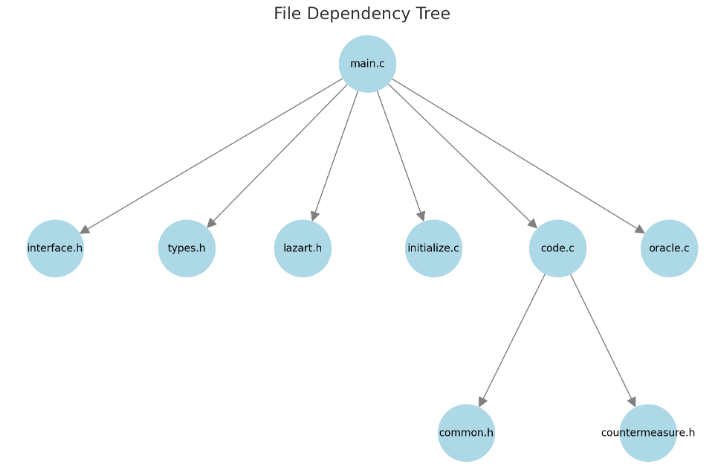
\includegraphics[width=0.75\linewidth]{Chapitre2/figures/tree.png}
    \caption{File dependency structure of the project. }
    \label{fig:file-tree}
\end{figure}

The program’s entry point resides in main.c in Listing\ref{main}, which handles system initialization(line 14), obtains user input—either simulated or fault-injected—and invokes the PIN validation logic(line 15) contained within the oracle module(line 16). The main function further processes the verification outcome and provides appropriate feedback(line 18 to 19). This file exemplifies typical control flow in embedded applications and is instrumental in assessing the resilience of entry and decision points under fault conditions.
\begin{figure}
\begin{lstlisting}[caption={main.c of VerifyPin function in benchmark V0}, label={main}, basicstyle=\ttfamily\footnotesize]
#include <stdio.h>
#include "interface.h"
#include "types.h"
#include "lazart.h"

extern UBYTE g_countermeasure;
extern BOOL g_authenticated;
extern SBYTE g_ptc;

BOOL verifyPIN(void);

int main()
{
    initialize();
    verifyPIN();
    LAZART_ORACLE(oracle());
    
    printf("[@] g_countermeasure = %i, g_authenticated = %x, g_ptc = %i\n", g_countermeasure, g_authenticated, g_ptc);
    return 0;
}
\end{lstlisting}
\end{figure}
The core decision-making logic is implemented in oracle.c in Listing\ref{oracle}, which performs a byte-wise comparison between the user-supplied PIN and the stored correct value. This approach mimics early-exit behaviors found in real-world implementations, offering exploitable points for differential fault analysis and side-channel attacks. The oracle deliberately omits certain protections such as masking or constant-time operations, making it a key target for both software- and hardware-based fault injections.
\begin{figure}
\begin{lstlisting}[caption={oracle.c of VerifyPin function in benchmark V0}, label={oracle}, basicstyle=\ttfamily\footnotesize]
#include "interface.h"
#include "types.h"

#ifdef AUTH
#define oracle_auth oracle
#endif

#ifdef PTC
#define oracle_ptc oracle
#endif

extern UBYTE g_countermeasure;
extern BOOL  g_authenticated;
extern SBYTE g_ptc;

BOOL oracle_auth()
{
    return g_countermeasure != 1 && g_authenticated == 1;
}

BOOL oracle_ptc()
{
    return g_countermeasure != 1 && g_ptc >= 3;
}
\end{lstlisting}
\end{figure}
Supporting utility functions are implemented in \texttt{code.c} (Figure~\ref{code}), including routines for memory comparison, data copying, and buffer manipulation. Although these functions are not directly exposed through external interfaces, they play a crucial role in shaping the program’s internal behavior and attack surface. Improper handling of memory within these helpers can introduce vulnerabilities, making them potential vectors for memory corruption attacks. Moreover, since these routines are reused across all benchmark versions, their correctness and security are essential for consistent evaluation and meaningful fault injection results.

To illustrate the core logic of the benchmark, we use version V0 as a representative example (Listing~\ref{code}). In this version, the program compares the user-entered PIN, stored in the variable \texttt{g\_userPin} (initialized to \texttt{"0000"}), with the correct card PIN, stored in \texttt{g\_cardPin} (initialized to \texttt{"4321"}). The PIN comparison logic simulates typical authentication behavior in embedded applications(line 29). Under normal conditions, the PINs do not match, and the program sets the \texttt{g\_authenticated} flag to \texttt{0}, indicating authentication failure(line 35). A successful fault injection attack can be detected when \texttt{g\_authenticated} is erroneously set to \texttt{1} despite the mismatch(line 31). The use of 0000 as the user input ensures a consistent and minimal binary pattern (all zeros), simplifying fault localization and enabling clear observation of bit flips or instruction corruption during the attack. Meanwhile, setting the card PIN to 4321 introduces a nontrivial comparison target with varied bit transitions, enhancing the likelihood of detecting successful bypasses or erroneous matches induced by injected faults. This contrast between the two values allows for precise control and clearer differentiation between correct and faulty program behavior in our analysis.

The number of permitted authentication attempts is managed by the variable \texttt{g\_ptc}, which is initialized to \texttt{3} and decremented after each failed attempt. Once \texttt{g\_ptc} reaches zero, further login attempts are blocked, simulating a basic protection against brute-force attacks. In the protected benchmark versions (V1 to V7), an additional countermeasure mechanism is introduced: when a fault is detected, a dedicated routine sets the variable \texttt{g\_countermeasure} to \texttt{1}. This mechanism enables the evaluation of the benchmark’s response to fault injection attempts, providing a clear indicator of whether the protection logic has correctly identified and responded to anomalous behavior.
\begin{figure}
\begin{lstlisting}[caption={code.c of VerifyPin function in benchmark V0}, label={code}, basicstyle=\ttfamily\footnotesize]
#include "interface.h"
#include "types.h"
#include "commons.h"

extern SBYTE g_ptc;
extern BOOL g_authenticated;
extern UBYTE g_userPin[PIN_SIZE];
extern UBYTE g_cardPin[PIN_SIZE];

#ifdef INLINE
__attribute__((always_inline)) inline BOOL byteArrayCompare(UBYTE* a1, UBYTE* a2, UBYTE size)
#else
BOOL byteArrayCompare(UBYTE* a1, UBYTE* a2, UBYTE size)
#endif
{
    int i;
    for(i = 0; i < size; i++) {
        if(a1[i] != a2[i]) {
            return 0;
        }
    }
    return 1;
}

BOOL verifyPIN() {
    g_authenticated = 0;

    if(g_ptc > 0) {
        if(byteArrayCompare(g_userPin, g_cardPin, PIN_SIZE) == 1) {
            g_ptc = 3;
            g_authenticated = 1; // Authentication();
            return 1;
        } else {
            g_ptc--;
            return 0;
        }
    }

    return 0;
}
\end{lstlisting}
\end{figure}
The initialization logic in initialize.c in Listing\ref{initialize} configures the program’s starting state by setting up internal data structures, initializing the correct PIN, and preparing buffers for interaction between the oracle and main program(line 21 to 28). This module ensures experiment reproducibility and consistency. Faults injected at this stage may induce persistent corruptions, making initialization a sensitive phase for certain attack types.
\begin{figure}
\begin{lstlisting}[caption={initialize.c of VerifyPin function in benchmark V0}, label={initialize}, basicstyle=\ttfamily\footnotesize]
#include "types.h"
#include "interface.h"
#include "commons.h"

// global variables definition
BOOL g_authenticated;
SBYTE g_ptc;
UBYTE g_countermeasure;
UBYTE g_userPin[PIN_SIZE];
UBYTE g_cardPin[PIN_SIZE];


void initialize()
{
   // local variables
   int i;
   // global variables initialization
   g_authenticated = 0;
   g_ptc = 3;
   g_countermeasure = 0;
   // card PIN = 1 2 3 4 5...
   for (i = 0; i < PIN_SIZE; ++i) {
       g_cardPin[i] = i+1;
   }
   // user PIN = 0 0 0 0 0...
   for (i = 0 ; i < PIN_SIZE; ++i) {
       g_userPin[i] = 0;
   }
}
\end{lstlisting}
\end{figure}
Basic protective features are implemented in countermeasure.c in Listing\ref{countermeasure}, simulating lightweight security mechanisms common in embedded applications. These include redundancy checks, sanity validations, and simple tamper detection routines. Though not exhaustive or production-grade, these countermeasures increase the complexity of the program’s state space and control flow, facilitating evaluation of attack strategies and security-performance trade-offs.
\begin{figure}
\begin{lstlisting}[caption={countermeasure.c of VerifyPin function in benchmark V0}, label={countermeasure}, basicstyle=\ttfamily\footnotesize]
#include "interface.h"
#include "types.h"

extern UBYTE g_countermeasure;

void countermeasure()
{
    g_countermeasure = 1;
}
\end{lstlisting}
\end{figure}
Types used throughout the benchmark, such as fixed-width integers (u8, u16, u32), are defined in types.h in Listing\ref{types}, promoting portability and deterministic behavior across platforms. This ensures consistent execution on both 32-bit and 64-bit systems, easing deployment in various simulation and hardware environments.
\begin{figure}
\begin{lstlisting}[caption={types.c of VerifyPin function in benchmark V0}, label={types}, basicstyle=\ttfamily\footnotesize]
#ifndef H_TYPES
#define H_TYPES
typedef signed char   SBYTE;
typedef unsigned char UBYTE;
typedef unsigned char BOOL;
typedef unsigned long ULONG;

#define BOOL_TRUE 0xAA
#define BOOL_FALSE 0x55

#endif // H_TYPES
\end{lstlisting}
\end{figure}
The interface between the core logic and external components is defined in interface.h, as shown in Listing~\ref{interface}. This header file specifies function prototypes and outlines the expected input/output data structures. It encapsulates the declarations of key functions, including the countermeasure, initialization, and oracle routines.
\begin{figure}
\begin{lstlisting}[caption={interface.h of VerifyPin function in benchmark V0}, label={interface}, basicstyle=\ttfamily\footnotesize]
#ifndef H_INTERFACE
#define H_INTERFACE

#include "types.h"

/* defines what happens when a fault has been detected
    implementation defined
*/
void countermeasure(void);

/* initializes global variables at the beginning of an example
    implementation-defined
    example-defined
*/
void initialize(void);

/* determines whether an attack is successful
    example-defined
*/
BOOL oracle(void);

#endif // H_INTERFACE
\end{lstlisting}
\end{figure}
Configuration options and compile-time toggles are centralized in lazart.h in Listing\ref{lazart} through macros controlling features such as debug printing, countermeasure activation, and early-return behavior. This allows flexible customization without altering the core code, enabling researchers to adjust program complexity and security levels for different test scenarios.
\begin{figure}
\begin{lstlisting}[caption={lazart.c of VerifyPin function in benchmark V0}, label={lazart}, basicstyle=\ttfamily\footnotesize]
#ifndef LAZART_API_HPP
#define LAZART_API_HPP

#ifdef LAZART

#include <klee/klee.h>

/*#define LAZART_ORACLE(oracle)               \
    if(oracle) {                            \
        klee_assume(oracle);                \
    } else {                                \
        klee_assume(0 != 0 );               \
    }*/

#define LAZART_ORACLE(oracle) klee_assume(oracle)

#else
#define LAZART_ORACLE(oracle)
#endif // LAZART

#endif // LAZART_API_HPP
\end{lstlisting}
\end{figure}
Shared constants, macros, and common includes are consolidated in commons.h in Listing\ref{commons} to improve maintainability and maintain consistency across files. This header typically contains global variables, debug settings, and high-level parameters, embodying best coding practices critical for modularity and clarity in embedded system development.
\begin{figure}
\begin{lstlisting}[caption={commons.c of VerifyPin function in benchmark V0}, label={commons}, basicstyle=\ttfamily\footnotesize]
#ifndef H_COMMONS
#define H_COMMONS

// macro definitions
#define INITIAL_VALUE 0x2a
#define PIN_SIZE 4

#endif // H_COMMONS
\end{lstlisting}
\end{figure}
In summary, VerifyPin V0 presents a compact yet comprehensive foundation for embedded software security analysis. The distinct roles of each source file—from user input handling and data verification to countermeasure implementation and configuration management—enable precise attack simulation, reproducibility, and adaptability. By exposing critical control and data flows, this benchmark serves as an effective tool for evaluating fault injection effects, validating detection mechanisms, and deepening the understanding of software vulnerabilities within constrained embedded environments.

\subsection{FISSA}
To efficiently handle the large number of simulations required for a comprehensive evaluation of the architecture's robustness, we employed FISSA (Fault Injection Simulation for Security Assessment)~\cite{PLG-24-dsd}, a Python-based tool specifically developed for generating and managing fault injection campaigns targeting microarchitectures. FISSA is designed to operate in conjunction with standard HDL simulators such as Questasim, Vivado, or Verilator, enabling users to conduct fault injection experiments within the same environment used for functional design and verification. This seamless integration supports both the validation of design functionality and the assessment of its resilience against physical fault injection attacks (FIA), thereby facilitating the development of effective countermeasures. In our work, we adopt the tool using the Questasim simulation backend and present the corresponding fault injection workflow.In this section, we provide a general introduction. The specific application of FISSA will be discussed in the next chapter.

\begin{figure}[t!]
  \centering
  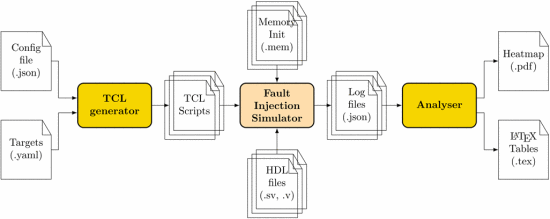
\includegraphics[width=0.5\linewidth]{Chapitre2/figures/fissa.png}
  \caption{FISSA component (source: \cite{PLG-24-dsd})}
  \label{fissa}
\end{figure}

FISSA is composed of three main components(Figure \ref{fissa}): the TCL Generator, the Fault Injection Simulator, and the Analyser. In our experiments, we utilize the first two components. The TCL Generator is responsible for producing the simulation scripts based on the specified configuration and fault parameters, while the Fault Injection Simulator executes these scripts to perform the actual simulations and generate structured log outputs for later analysis.

The TCL script generation process is driven by a set of Python classes, each responsible for producing portions of the final output scripts. The process begins with an initialisation class that extracts parameters from a JSON-formatted configuration file. This file specifies key simulation settings, including the HDL simulator to be used, the fault model, injection window(s), the design’s clock period (in nanoseconds), and the maximum number of simulation cycles allowed before forced termination in case of divergence. It also defines the number of simulations to be included in each TCL file, which determines the degree of parallelism in simulation execution.

In addition to the configuration file, a separate YAML-formatted targets file lists the elements of the circuit to be faulted—such as registers or logic gates—along with their HDL paths and bit-widths. These targets are essential inputs to the fault injection campaign.

Based on the configuration and target data, the TCL Script Generator class coordinates the creation of complete TCL scripts. It delegates specific tasks to three auxiliary classes. The Basic Code Generator produces the core TCL instructions to initialize, run, and terminate a simulation. The Fault Generator creates TCL code that defines fault injection operations, using parameters that specify target elements and fault injection clock cycles. The Log Generator outputs TCL code for automated logging of simulation metadata, including simulation ID, fault model, faulted elements, injection time, status at simulation end, values of all targets, and the final simulation cycle.

Each TCL file corresponds to a batch of simulations and begins with a reference simulation without fault injection. This enables result comparison within each batch. Additionally, a standalone target file is generated for TCL scripts to retrieve the fault injection targets.

The Fault Injection Simulator operates by leveraging an existing HDL simulator, which executes the TCL scripts generated during the previous stage. For each simulation, a corresponding log file is produced in JSON format, capturing essential metadata such as the simulation index, the number of clock cycles executed, the values from the target file, the faulted elements, the applied fault model, and the final simulation status.

To ensure seamless integration within the designer’s existing workflow, the invocation of these TCL scripts must be incorporated into the broader design process. This includes stages such as design compilation, initialization, and input stimulus management. The script-based approach facilitates this integration by providing a modular and automated interface to the simulation environment.

After completing all fault injection campaigns, the resulting log files are passed to the Analyser component, which is introduced in the following subsection.

\subsection{Attack model}

In this study, we define a realistic and constrained fault injection threat model tailored for the evaluation of embedded security mechanisms under simulation. The attacker operates in a black-box setting, with no knowledge of the correct PIN value stored in the system, which is initialized as \texttt{"4321"} in all test cases. The input PIN, set to \texttt{"0000"}, is deliberately incorrect to ensure that any successful authentication outcome can be attributed solely to fault-induced corruption. This assumption reflects practical attack scenarios where the attacker is unable to retrieve or infer secret values through direct observation.

Fault injection is performed within a simulation environment using TCL commands generated by the FISSA tool. These commands emulate physical fault attacks at the register-transfer level (RTL), injecting faults into specific control elements during simulation time. The attack campaign is automated and covers multiple clock cycles corresponding to the execution of the \texttt{verifyPIN} function \ref{code} and the targeting of critical registers, providing a broad view of the system’s vulnerability to transient faults. In order to evaluate the robustness of the architecture under a diverse range of attack scenarios, we also introduced different-level-complexity fault models predefined in FISSA (Figure \ref{fault model}). The considered models are all single-cycle attacks:
\begin{enumerate}
\item Bit-Flip: 1 bit-flip in register.
\item Manipulate Register: This model allows arbitrary bit-flips in any single register. Both the number of flipped bits and their positions within the register are unrestricted, simulating a wide range of fault patterns within a single storage element.
\item 2 Bit-Flips: This model restricts fault injection to exactly two bit-flips. The two flipped bits may occur within the same register or across two different registers. This model is designed to represent dual-bit fault scenarios, such as multi-bit upsets (MBUs) induced by radiation or other environmental factors.
\item Manipulate Two Registers: This model extends the manipulation to two distinct registers, where each register can experience arbitrary numbers of bit-flips at arbitrary positions. This model captures complex fault cases involving simultaneous corruption across multiple storage elements.
\end{enumerate}

\begin{figure}[t!]
  \centering
  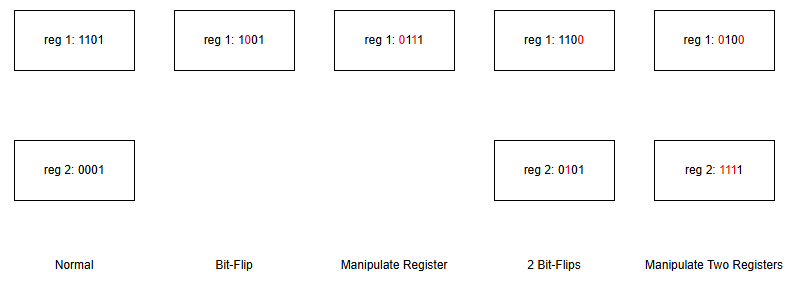
\includegraphics[width=0.5\linewidth]{Chapitre2/figures/fault model.png}
  \caption{Example of 4 fault models}
  \label{fault model}
\end{figure}

According to the article\cite{sass2023oops}, the models are constrained to generate at most four faults, which is deemed adequate for capturing the dominant classes of fault injection behavior observed in practical systems. These diversified fault models enable more comprehensive coverage of possible fault manifestations and allow finer-grained analysis of the architecture’s fault tolerance capabilities.

The scope of the attack is intentionally limited to control registers connected to the system bus, excluding data and address lines. This restriction reflects common architectural protections: in many embedded systems, address and data buses are either not latched in vulnerable registers or are protected through error detection and correction (EDC) mechanisms, such as parity bits or ECC codes. As such, targeting them in fault injection campaigns would either be ineffective or unrepresentative of realistic fault propagation paths. By focusing on control registers—such as status flags, authentication result indicators, or loop counters—we model an attacker capable of subtly influencing the control flow of the software without inducing immediate system crashes or violating low-level bus protocols.

A fault is considered successful if it leads to an unauthorized authentication, i.e., the variable \texttt{g\_authenticated} is incorrectly set to \texttt{1} despite the incorrect input PIN. Importantly, successful faults must not cause the system to halt, crash, or enter undefined behavior states. Furthermore, in protected versions of the benchmark (V1 to V7), any such fault must also evade detection or correction by the implemented countermeasures. To systematically analyze the effects of fault injection, the simulation results were categorized into five distinct outcomes:
\begin{enumerate}
\item Crash, the simulation either exceeded the fixed execution time or triggered a crash signal, resulting in termination.
\item Detect, the fault was detected by the countermeasure, setting the variable \texttt{g\_countermeasure} to "1".
\item Success, the authentication bypassed successfully, with \texttt{g\_authenticated} set to "1".
\item Change, no successful authentication or detection occurred, but the memory state was altered by the fault.
\item Silence, no authentication success, detection, or memory state change was observed, indicating the fault had no visible impact.
\end{enumerate}
Among these, only the “Success” outcome, defined as the achievement of unauthorized authentication without detection or system failure, qualifies as a valid and exploitable fault from an attacker’s perspective.

The system under test incorporates both hardware and software countermeasures. Hardware-level protections may be embedded in the Verilog design of the system, including fault-tolerant state machines or error-detection logic at the bus interface. On the software side, the VerifyPin benchmark provides seven protected implementations (V1–V7), each incorporating a different strategy to detect or tolerate fault effects—ranging from control flow integrity checks to redundant variable encoding.

This threat model allows for controlled and repeatable evaluation of the system’s security posture under targeted, register-level fault injection, providing valuable insight into the effectiveness of different defensive strategies and the residual risks that remain even under constrained attacker capabilities.

\section{Conclusion}
In summary, this chapter has established a comprehensive experimental framework for evaluating fault-based attacks targeting SoC interconnects. By detailing the SoC architecture, bus configurations, attacker model, and fault injection methodology, we have laid the technical groundwork for systematic and reproducible analysis. The integration of configurable benchmarks and clear evaluation metrics further enables meaningful comparisons across different protection strategies and fault scenarios. Building on this foundation, the next chapter delves into the exploitation of vulnerabilities specific to the communication buses under study—namely, Wishbone, AXI-Lite, and AXI—demonstrating how carefully crafted fault injections can compromise data integrity, control flow, and system behavior across these widely-used protocols.


\clearemptydoublepage
\chapter{Vulnerabilities exploitation on the bus: wishbone, AXI-Lite et AXI}
Building on the previously established experimental setup, this chapter investigates the vulnerabilities of three widely used SoC bus protocols—Wishbone, AXI-Lite, and AXI—under fault injection attacks. These interconnects play a central role in processor-memory communication and are potential points of failure when exposed to transient faults. We briefly introduce each protocol's relevant features, followed by targeted fault injection experiments designed to assess their resilience. By comparing their behavior under similar fault scenarios, we identify protocol-specific weaknesses and extract general insights into bus-level fault tolerance.
\section{Introduction of bus}

\subsection{Wishbone}
We conducted an in-depth examination of each signal within the Wishbone bus, referencing their definitions from the official Wishbone specification. By analyzing the Verilog source code, inspecting Vivado’s elaborated design, and consulting publicly available diagrams~\cite{wishbonewiki}, we assembled a modular SoC architecture that explicitly delineates the Wishbone interconnect and its peripheral components.

The overall structure is depicted in Figure~\ref{architecturebus}. Data transmission is handled by \texttt{DAT\_I} (data input) and \texttt{DAT\_O} (data output), enabling bidirectional communication between the processor and memory modules. Address targeting is managed via \texttt{ADR\_O}, which designates the intended memory address. Control signals include \texttt{WE\_O} (write enable) to indicate write cycles, \texttt{STB\_O} (strobe) to signal valid operations, and \texttt{CYC\_O} (cycle) to initiate active bus phases. Handshaking is achieved through \texttt{ACK\_I} (acknowledge signal), which validates the completion of a data transaction. Byte-level data access is supported by \texttt{SEL\_O} (byte select). Additionally, \texttt{CLK\_I} supplies the system clock, while \texttt{RST\_I} resets the bus interface for proper startup. Certain extended implementations also incorporate \texttt{TAGN\_O} and \texttt{TAGN\_I}, used to convey auxiliary metadata for advanced bus operations.

\begin{figure}[t!]
  \centering
  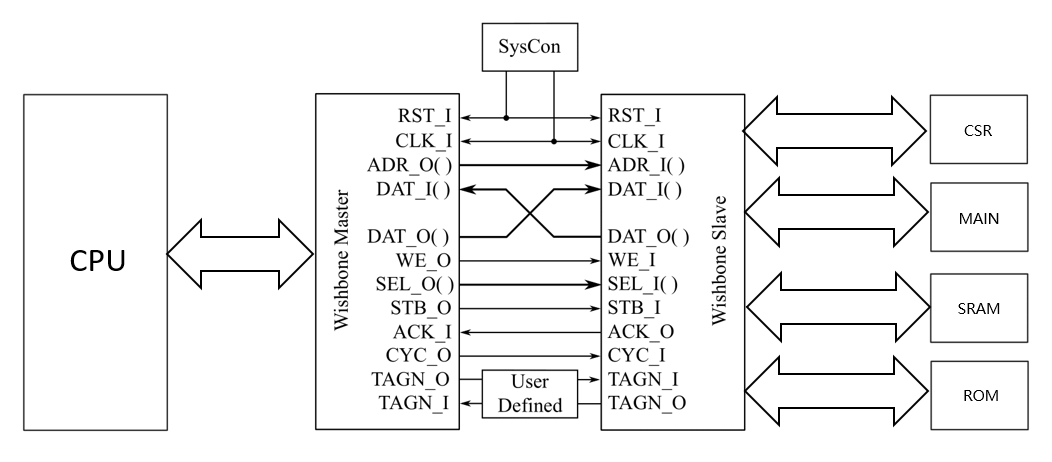
\includegraphics[width=\linewidth]{Chapitre3/figures/Wishbone.png}
  \caption{Signals exchange between CPU and memory via Wishbone bus}
  \label{architecturebus}
\end{figure}

Data transfer operations rely on the configuration of control registers. Here, we highlight two of the most critical: \texttt{SEL} and \texttt{ACK}.

The \texttt{SEL} register (Figure~\ref{sel}) is a 4-bit selector, with each bit corresponding to one of four memory blocks. It functions as a memory selection indicator, specifying which memory module the CPU interacts with during data access. The \texttt{SEL} value is derived from the address register \texttt{ADR} through combinational logic, represented by the shaded cloud region in Figure~\ref{sel}. Each bit in \texttt{SEL} is expanded to match the data width (32 bits) and passed through a series of AND gates. The outputs are then merged via OR gates to produce the final read result. During a read or write operation, only the bit in \texttt{SEL} corresponding to the targeted memory is set to \texttt{1}, ensuring that data from only the selected memory block is forwarded through the logic and accessed by the CPU.

The \texttt{ACK} mechanism (Figure~\ref{ack}) includes four individual 1-bit acknowledge signals (each ending with \texttt{ACK}), each maintained in a dedicated register. The input to each acknowledge line is generated through a logical AND operation involving its previous value, the \texttt{STB} and \texttt{CYC} control signals, and the corresponding bit of the \texttt{SEL} register. These four acknowledge outputs are then combined using OR logic to produce a shared signal. This shared signal is further processed by performing an AND with both the grant register and its inverted form, yielding the response signal for data and instruction paths respectively. These response signals are fed back to the CPU, coordinating address updates and controlling the data transaction timing.

\begin{figure}[t!]
  \centering
  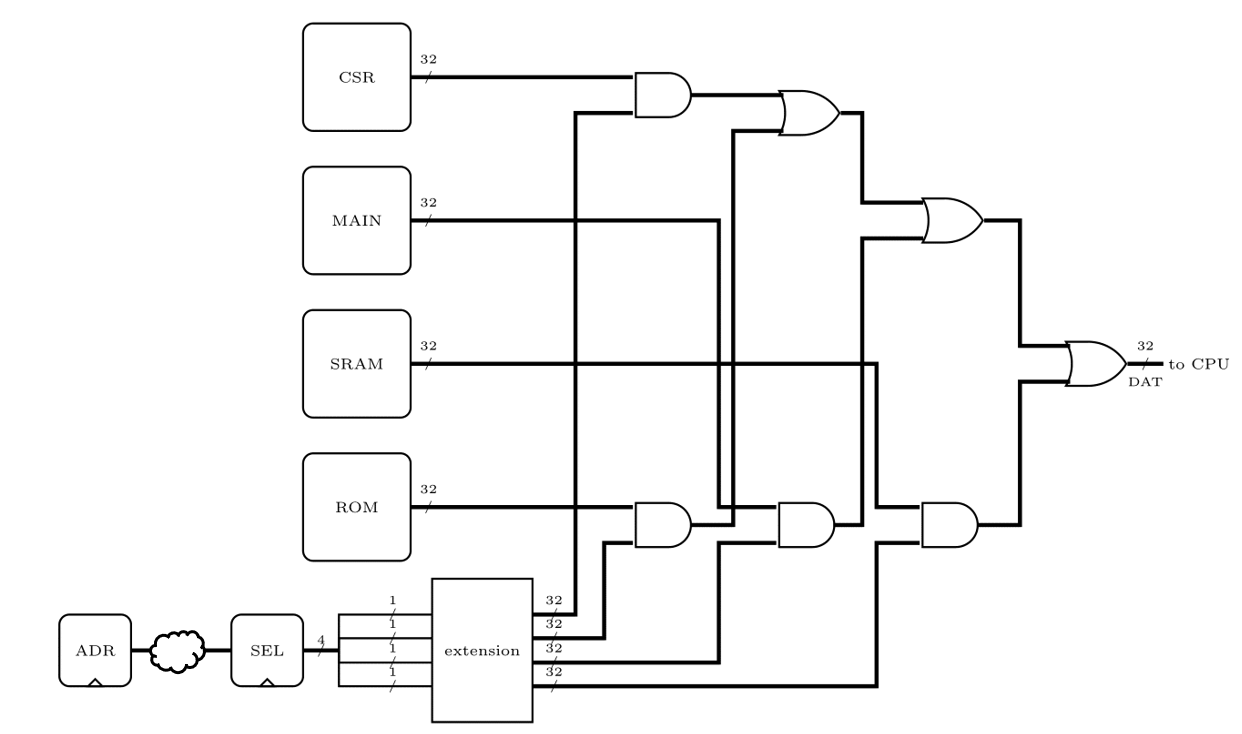
\includegraphics[width=1.1\linewidth]{Chapitre3/figures/sel.png}
  \caption{Connection of selection register with CPU and memory on the bus}
  \label{sel}
\end{figure}

\begin{figure}[t!]
  \centering
  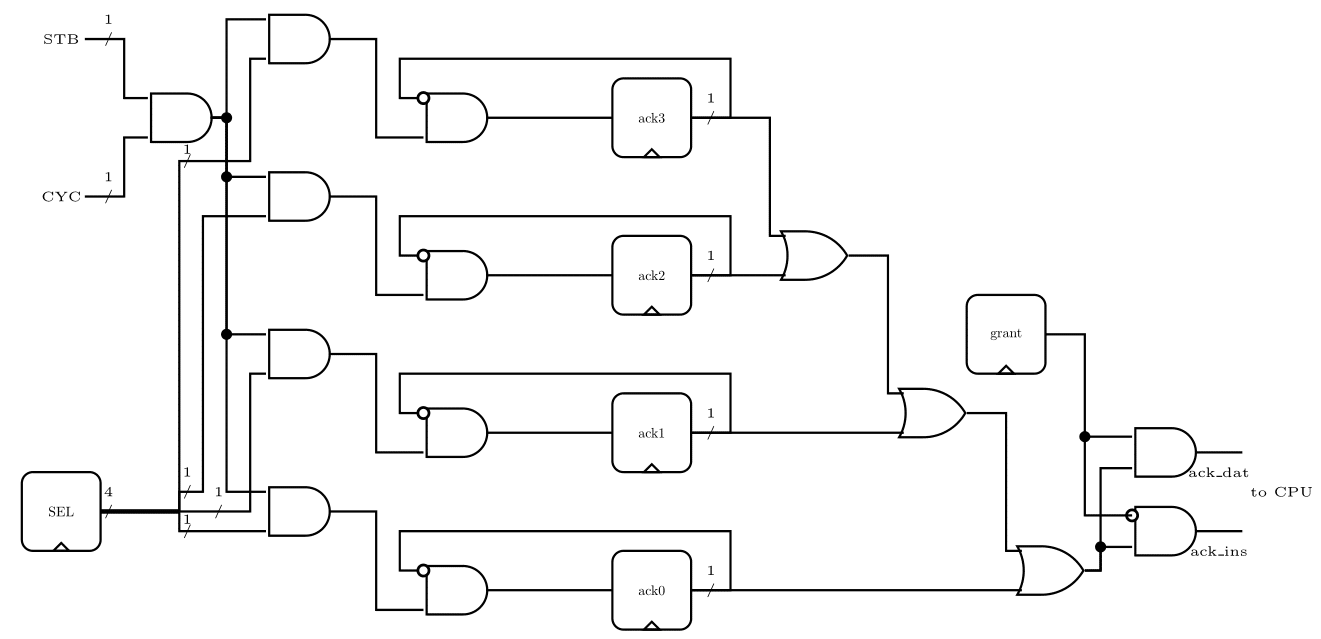
\includegraphics[width=1.1\linewidth]{Chapitre3/figures/ack.png}
  \caption{Connection of acknowledge registers with address registers and memory on the bus}
  \label{ack}
\end{figure}

The Wishbone bus protocol specifies a straightforward, synchronous communication scheme between a single master and one or more slave devices. Figure~\ref{nofault} illustrates the signal behavior during a typical read operation. In systems featuring multiple masters, each transaction begins with an arbitration phase, during which masters must request access to the shared bus. Access is granted via a \texttt{grant} signal issued by the arbiter. In this figure, \texttt{grant} is asserted (\texttt{1}), indicating that the transaction involves data rather than an instruction. This mechanism ensures mutual exclusion by allowing only one master to initiate communication at any given time. In systems with a single master, this arbitration step is bypassed, and the master can initiate a transaction immediately.

Upon receiving bus access, the master asserts \texttt{cyc} (cycle valid) to initiate a valid bus cycle and sets \texttt{stb} (strobe) to indicate a data transfer request. Concurrently, it places the target address on the \texttt{adr} lines and specifies the operation type using the \texttt{we} (write enable) signal: \texttt{we = 1} for a write, and \texttt{we = 0} for a read. In the case of a write, the data is placed on the \texttt{dat\_w} bus (not shown in this figure). These signals collectively define the operation parameters.

The addressed slave monitors the \texttt{cyc} and \texttt{stb} lines. Upon detecting a valid transaction, it responds by asserting \texttt{ack} (acknowledge). In the example shown, \texttt{cyc} and \texttt{stb} are both high, enabling \texttt{ack0}. The acknowledge lines \texttt{ack0} through \texttt{ack3} are OR-combined to form \texttt{ack\_all}, which is selected by the \texttt{grant} signal to produce the data acknowledgment signal \texttt{ACK\_D} and instruction acknowledgment signal \texttt{ACK\_I}. In Figure \ref{architecturebus} we gather these two signals as acknowledgment  signal\texttt{ACK\_I}. This signal confirms the slave has accepted the write or that valid read data is available on \texttt{dat\_r} (labeled \texttt{DAT} in the figure). The \texttt{sel} signal determines which memory block is addressed by the CPU. Here, \texttt{sel = 0010}, indicating that \texttt{dat1} is routed to \texttt{DAT} and forwarded to the CPU cache. Once the master receives \texttt{ACK\_D}, the transaction is complete: for reads, it captures the data on \texttt{dat\_r}; for writes, the operation concludes upon acknowledgment reception. The master may then deassert \texttt{stb} to end the current transfer or \texttt{cyc} to terminate the bus cycle entirely.

After deassertion, the slave releases the \texttt{ack} line, and the bus returns to an idle state. In multi-master environments, the arbiter may now allocate the bus to another requester via the \texttt{grant} mechanism, restarting the communication sequence.

Although this handshake-driven protocol ensures predictable, clock-synchronous communication, it also exposes potential vulnerabilities under fault injection scenarios. For example, if a transient fault prematurely triggers \texttt{ack} or activates \texttt{grant} erroneously, a master may proceed without legitimate access or before the slave is ready. This can lead to data corruption, unintended memory access, or desynchronization between components. Such risks emphasize the importance of protecting arbitration logic and critical control signals in high-assurance systems.

\begin{figure}[t!]
  \centering
  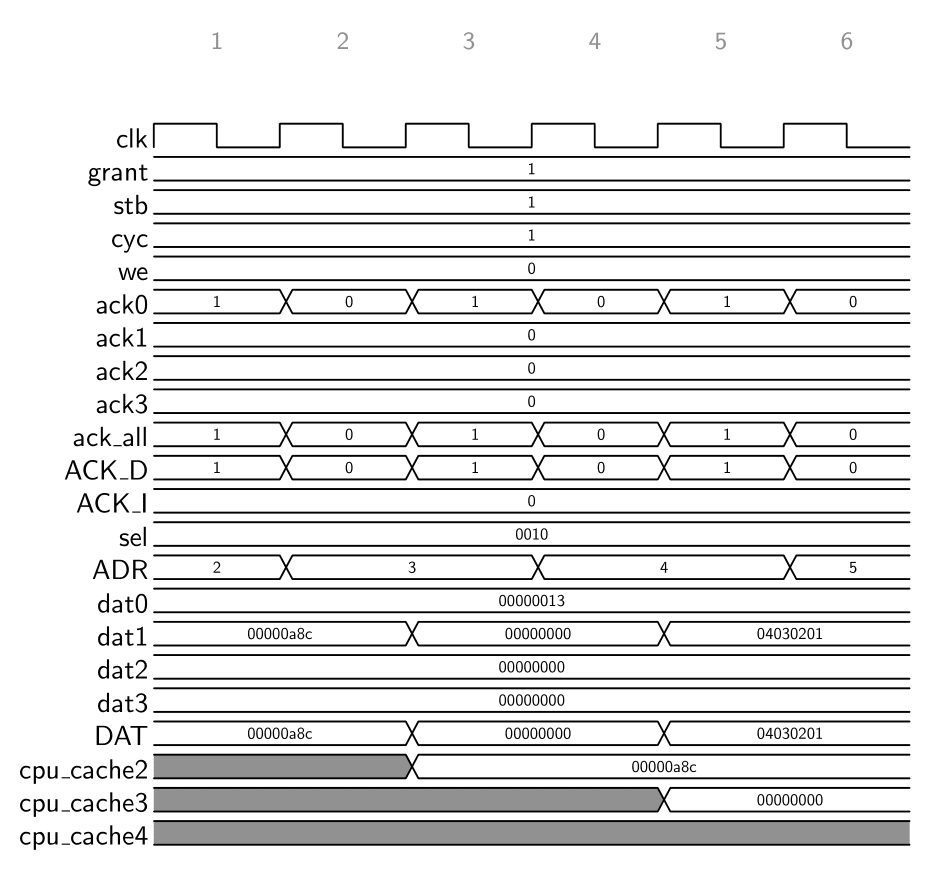
\includegraphics[width=\linewidth]{Chapitre3/figures/nofault.png}
  \caption{Impact of signal transportation without attack in Wishbone}
  \label{nofault}
\end{figure}

\subsection{AXI-Lite}
The AXI-Lite protocol defines a simplified, synchronous communication interface that connects a single master to one or more slave components through a set of well-structured signal channels. This protocol is primarily intended for low-latency, memory-mapped register access within system-on-chip (SoC) architectures, offering a streamlined approach to peripheral communication.

Data exchange in AXI-Lite is orchestrated across five logically independent, unidirectional channels: write address, write data, write response, read address, and read data. Each channel operates using a handshake mechanism built upon two control signals—\texttt{VALID} and \texttt{READY}—that coordinate data transfer. A transaction occurs only when both signals are asserted high, ensuring synchronous and deterministic communication between the master and the slave.

In a write transaction, the master initiates communication by presenting the destination address on the \texttt{AWADDR} signal and setting \texttt{AWVALID} to indicate that the address is ready for sampling. The slave acknowledges its readiness via \texttt{AWREADY}, at which point address transfer is considered complete. Next, the master provides the actual data over the \texttt{WDATA} line, accompanied by the write strobes (\texttt{WSTRB}) that specify active byte lanes, and raises \texttt{WVALID} to signal valid data. The slave asserts \texttt{WREADY} when it is prepared to accept the data. After internal processing, the slave returns a response using the write response channel by asserting \texttt{BVALID} and driving the \texttt{BRESP} signal to indicate the status of the write. The master concludes the transaction by asserting \texttt{BREADY}, acknowledging receipt of the response.

Read transactions follow a similar handshake-based sequence. We present in Figure\ref{axilite}. The master asserts a target read address on \texttt{ARADDR} along with \texttt{ARVALID}, signaling a valid read request. The slave responds with \texttt{ARREADY}, confirming address acceptance. After processing, the slave places the requested data on the \texttt{RDATA} bus (named as \texttt{DAT} in the figure), provides a response code via \texttt{RRESP} (named as \texttt{r\_resp} in the figure), and asserts \texttt{RVALID} (named as \texttt{r\_valid} in the figure) to indicate valid output. The master completes the operation by asserting \texttt{RREADY} (named as \texttt{r\_ready} in the figure), allowing the data and response to be captured.

Each signal in the AXI-Lite protocol has a clearly defined role: address lines (\texttt{AWADDR}, \texttt{ARADDR}) designate the transaction target; data lines (\texttt{WDATA}, \texttt{RDATA}) carry payloads; strobe (\texttt{WSTRB}) selects byte lanes during writes; response signals (\texttt{BRESP}, \texttt{RRESP}) indicate transaction results; and the handshaking signals (\texttt{VALID}, \texttt{READY}) synchronize all transfers without ambiguity. This explicit signal-level orchestration ensures reliable communication, even in timing-constrained environments.

Similar to the Wishbone protocol, the response and selection mechanisms in AXI-Lite govern both the timing and the granularity of data transfers. In standard AXI-Lite implementations, the response signal \texttt{BRESP} is used for write transactions, while \texttt{RRESP} is used for read responses and directly connects to the CPU. However, in the bus architecture generated by LiteX, both \texttt{BRESP} and \texttt{RRESP} are internally mapped to an \texttt{ack} signal, which is subsequently routed to the CPU interface. While the Wishbone protocol explicitly defines \texttt{ACK} and \texttt{SEL} as separate signals, their equivalent functionality in AXI-Lite is implicitly realized through a combination of richer control signals, including \texttt{VALID}, \texttt{READY}, and \texttt{WSTRB}. These signals coordinate transaction sequencing and enable byte-level selection during data transfers, thereby replicating the behavior of traditional acknowledgement and selection lines in a more integrated manner.

\begin{figure}[t!]
  \centering
  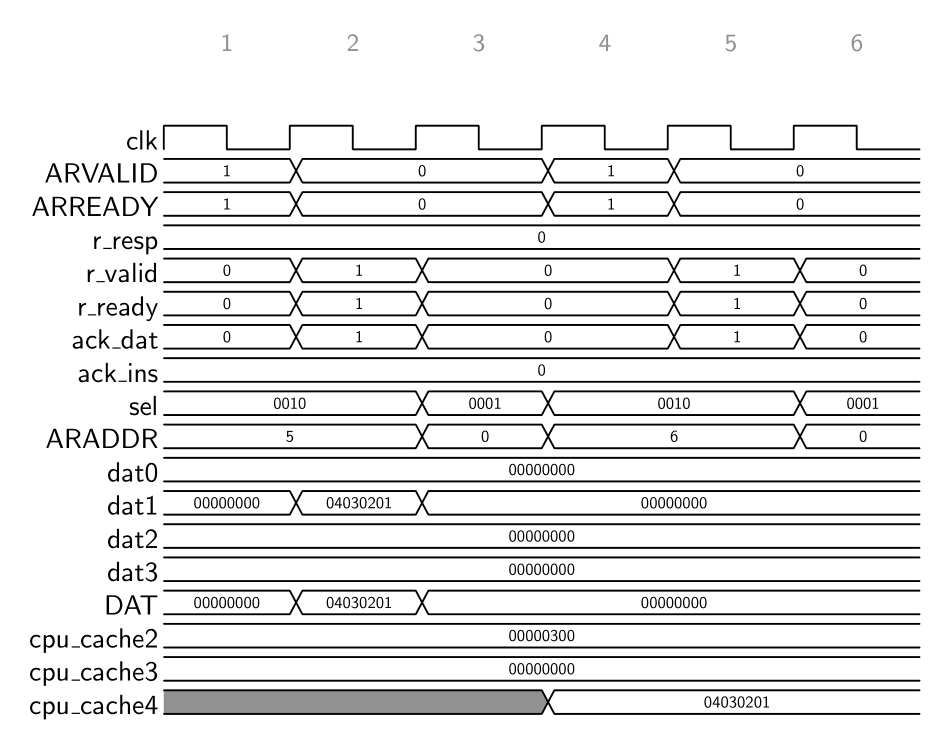
\includegraphics[width=\linewidth]{Chapitre3/figures/axilite.png}
  \caption{Impact of signal transportation without attack in AXI-Lite}
  \label{axilite}
\end{figure}

In addition, we observed that the AXI-Lite bus generated by LiteX introduces a clearing mechanism for improved bus consistency. Specifically, when a particular data channel is active during a read transaction, other unrelated data buses are automatically cleared by setting their values to zero. Furthermore, in the event of a detected fault or error on the bus indicated by state register, read and write data bus is also cleared to zero, and the \texttt{ACK} signal is asserted to indicate that a transaction has been completed, albeit unsuccessfully. This behavior ensures deterministic responses under error conditions and prevents the propagation of invalid data, thereby contributing to system robustness.

Given its predictable behavior and well-defined signaling model, AXI-Lite is particularly suitable for configuration registers, low-bandwidth control paths, and secure interactions between software and hardware components. A thorough understanding of each signal's function within the data transaction phases is essential when implementing or analyzing system interfaces, particularly in contexts such as verification, debugging, or fault injection analysis.

\subsection{AXI}
The AXI (Advanced eXtensible Interface) protocol offers a comprehensive and high-performance interconnect solution within the AMBA specification family. It supports burst-based data transfers, out-of-order transaction handling, and parallel communication from multiple master devices. In contrast, AXI-Lite represents a streamlined variant tailored for low-throughput register-level access, such as configuration or control registers. The two differ significantly in structure and capability. AXI enables multi-beat transfers through parameters like \texttt{AWLEN} and \texttt{AWSIZE}, maintains independent channels for address and data phases, and allows for flexible response ordering. AXI-Lite eliminates these advanced features, restricting all transactions to single-beat operations and reducing the number of control and handshake signals. As a result, AXI-Lite is lightweight, easier to implement, and occupies less silicon area, making it suitable for interfacing with peripheral components. Meanwhile, full AXI is typically used in bandwidth-intensive modules, such as memory subsystems or high-speed I/O. In system-on-chip designs, AXI is often reserved for core interconnects, while AXI-Lite is employed for peripheral configuration paths. Because there are so many features, there are more registers on the AXI.

Similar to the AXI-Lite protocol, the AXI protocol employs response and selection mechanisms to manage the timing and granularity of data transfers. However, in AXI, these mechanisms are significantly more complex and feature-rich. The protocol supports multiple outstanding transactions, burst transfers, and out-of-order responses, requiring a more sophisticated structure for handshaking, address decoding, and response signaling. This added complexity enhances throughput and flexibility but also introduces additional challenges in implementation and verification.

In addition, the AXI interconnect generated by LiteX incorporates a clearing mechanism aligned with AXI-Lite semantics. During a read transaction, when one data channel is actively in use, other unrelated data buses are automatically zeroed out to prevent residual or unintended values. If a fault or error condition is detected—typically flagged by a system state register—the read and write data lines are forcefully cleared to zero. In such cases, the \texttt{ACK} signal is still asserted to mark the end of the transaction, even though it may have failed, thus ensuring protocol completion and preventing bus deadlock.

\section{Vulnerable test on bus}

Following the detailed overview of the Wishbone, AXI-Lite, and AXI bus protocols, the next section focuses on conducting fault injection experiments targeting these three interconnects. By simulating various fault scenarios, we aim to evaluate how each bus architecture responds to disruptive conditions, highlighting their respective resilience and vulnerability. These experiments serve to validate the theoretical analysis presented earlier and provide practical insights for designing more robust countermeasures.

\subsection{Aim}

To systematically assess the inherent robustness of various bus architectures against fault injection, we begin by targeting the Wishbone, AXI-Lite, and AXI buses in their default, unprotected configurations—without any hardware or software countermeasures in place. To eliminate hardware-level protection, we employ the original SoC architecture without added shielding or error-checking logic. To exclude software-level defenses, we use version v0 of the VerifyPin benchmark, which contains no built-in fault detection or recovery mechanisms. This baseline testing phase establishes a neutral, protocol-independent foundation for comparing the fault tolerance characteristics of the three interconnects. All experiments are conducted using consistent fault models and synchronized trigger conditions to ensure fairness and reproducibility. The objective is to observe how transient faults propagate across each bus interface and influence system behavior in the absence of any protective layers. This analysis is essential for exposing the underlying architectural vulnerabilities and for providing a reference point against which the effectiveness of subsequent countermeasure implementations can be measured.

In analyzing successful fault injections across the three bus architectures, we examine several dimensions: the specific registers impacted, the timing windows in which faults are most effective, and whether data or instruction paths are corrupted. While all three buses demonstrate sensitivity to timing-accurate fault injection near transaction boundaries, differences emerge in how and where faults manifest. For example, AXI—with its decoupled read/write channels and handshake signals—shows delayed but wider impact, often corrupting data during burst transfers. In contrast, Wishbone's simpler handshaking and tighter coupling between control and data lead to more localized fault effects, usually within specific instruction or configuration registers. AXI-Lite, being structurally simpler than full AXI but more modular than Wishbone, shows an intermediate pattern. The analysis reveals how bus topology, signal granularity, and transaction sequencing influence the propagation of transient faults and determine the specific functional units affected.

To further differentiate the fault resistance of each bus, we evaluate three experimental metrics: the practical difficulty of injecting effective faults, the overall time required to conduct the campaign, and the number of distinct registers successfully targeted. AXI buses, due to their protocol complexity and the presence of multiple timing domains, typically require more precise injection strategies, increasing the difficulty and experimentation time. However, they also expose a wider attack surface, particularly in burst or pipelined operations. Wishbone, though easier to disrupt due to its predictable signaling and simpler timing, exhibits fewer exploitable registers in a given test case. AXI-Lite lies in between, both in complexity and fault injection difficulty. This comparative study allows us to quantify the attack feasibility for each bus type and prioritize countermeasure deployment based on vulnerability density and ease of exploitation.

\subsection{Step}

We perform the fault injection experiments according to the following procedure. First, we generate the System-on-Chip (SoC) architectures using LiteX, configured as described previously. Specifically, we generate three distinct SoC variants—each using one of the three bus protocols: Wishbone, AXI-Lite, and AXI. These designs maintain consistent CPU and peripheral configurations to ensure fair comparison. Subsequently, the \texttt{VerifyPin} benchmark (version v0), originally written in C, is compiled into a binary file without optimization flags, preserving the instruction-level structure for fault sensitivity.

The resulting binary is then embedded into each SoC variant. Corresponding bitstreams are generated and programmed onto an FPGA development board to validate the correctness of each hardware design under real-world deployment. This hardware verification step ensures that each bus protocol can support basic program execution without protection mechanisms.

In parallel, we initiate a simulation-based workflow using the Verilog source files and memory initialization files generated by LiteX for each SoC. Our first step is to verify that the designs can be successfully compiled and simulated. During this stage, we observe numerous redundant or duplicated signal assignments, particularly in the AXI-Lite and AXI architectures. These redundancies are introduced by LiteX’s automatic code generation process. In the case of AXI-Lite and AXI buses, we encounter compilation errors due to signal redriving, which violate synthesis rules. We address this by manually identifying and removing the redundant statements in an iterative process. Each modification is followed by recompilation to ensure correctness.

Once the designs are successfully compiled, we proceed to simulate all three architectures. Initially, we observe incorrect behavior in program execution. This issue is traced to subtle incompatibilities between the memory layout and the binary. We resolve this by modifying the C source of \texttt{VerifyPin}, recompiling it into a new binary, and converting it again into an initialization file. We then re-integrate this file and verify correct execution through simulation.

To further ensure simulation accuracy and prevent undefined behavior due to uninitialized memory, we explicitly initialize all memory components—except for ROM—with zero values using the assignment \texttt{32'h00000000}. This eliminates the propagation of X-type logic states during simulation, which could otherwise corrupt bus behavior or control signals.

Next, we analyze the internal structure of each SoC to understand how the bus interconnect behaves under normal execution. Using Vivado's elaborated design visualization, we generate detailed RTL schematics for all three designs. These diagrams provide a global overview of the SoC and enable us to classify its components into three functional domains: the CPU core, the bus interconnect, and peripheral memory regions. Based on signal connections and naming conventions, we identify the key registers within each region.

We further categorize all bus-connected registers based on their name, bit-width, and role within the data flow. Registers are grouped into three major types: data-related, address-related, and control-related. This classification allows us to narrow down potential fault injection targets.

After enumerating and analyzing the register set, we exclude certain classes of registers from our attack scope. First, registers storing raw data or memory addresses are ignored, as these can be protected using data integrity mechanisms such as error detection codes or mirrored verification logic between CPU and memory, as discussed in the literature. Secondly, registers controlling the clock and reset logic are also excluded, since clock-glitching attacks on them have already been comprehensively explored. Moreover, since our experiments are conducted entirely within a single SoC instance in simulation, we ignore registers responsible for I/O functions such as LEDs and UART RX/TX interfaces. Finally, we experimentally verify that faulting the Timer-related registers does not affect program control flow in our benchmark, so these are also excluded.

The structure of our attack model is illustrated in Figure~\ref{general}. The figure provides a simplified overview of the SoC’s communication architecture, featuring a central processor and multiple memory-mapped peripheral blocks. Data exchange between the CPU and memory regions—including ROM, RAM, and CSR (which contains the UART and Timer modules)—is conducted via a shared bus. The communication is categorized into three signal domains: data signals (represented in green), address signals (yellow), and control signals (blue). A key control signal, \texttt{SEL}, determines which memory module is accessed during a read or write operation. It achieves this by driving a multiplexer composed of combinational logic. Another crucial signal, \texttt{ACK}, is responsible for handshaking with the CPU to synchronize memory access timing and indicate transaction completion. The precise architecture of these two signal will be presented in next chapter.

\begin{figure}[t!]
  \centering
  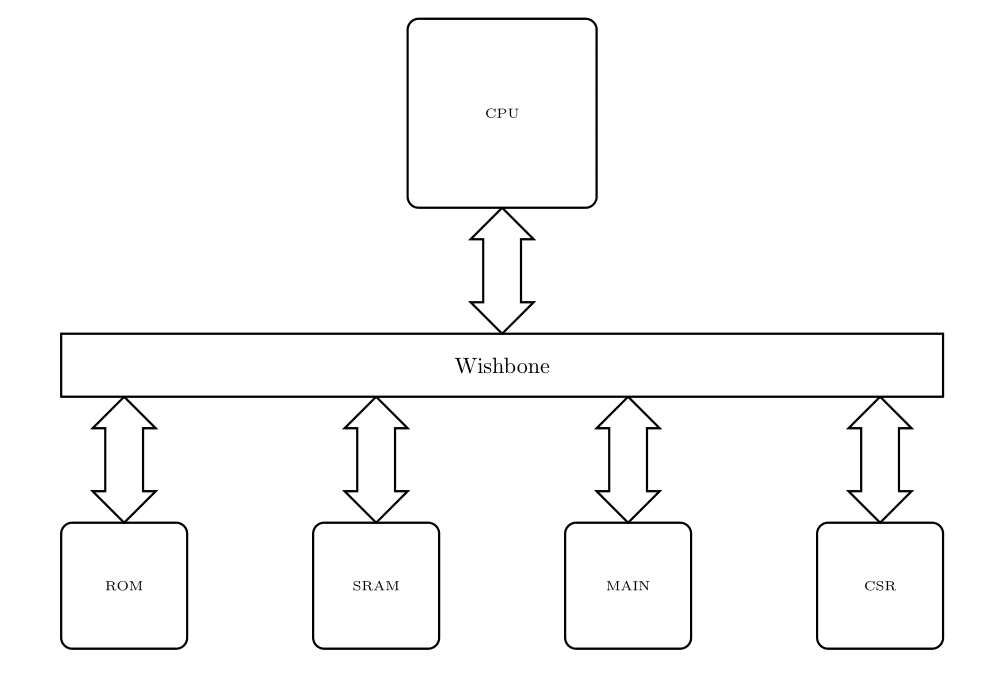
\includegraphics[width=\linewidth]{Chapitre3/figures/general.png}
  \caption{General structure of the SoC and bus}
  \label{general}
\end{figure}

To generate the required simulation scripts, we employ the FISSA tool, which outputs a set of Tcl commands based on the configuration defined in a JSON file. As illustrated in Figure~\ref{conf}, the configuration file \texttt{config\_wop.json} allows users to customize a wide range of parameters to tailor the fault injection campaign.

The parameter \texttt{name\_simulator} specifies the simulation engine in use—such as ModelSim in our case. A group of path-related variables—namely \texttt{path\_tcl\_generation}, \texttt{path\_files\_sim}, \texttt{path\_generated\_sim}, \texttt{path\_results\_sim}, and \texttt{path\_simulation}—are used to define the respective directories: where the FISSA tool is located, where the necessary simulation input files reside, where the generated Tcl scripts are saved, where the simulation results are stored, and where the Verilog-based simulation project is hosted.

The \texttt{threat\_model} field determines the type of attack scenario being used. In our study, four different models are evaluated; the one shown in the figure is the 2-bit-flip attack, denoted in FISSA as \texttt{single\_bitflip\_spatial}. This model simulates spatially localized bit-flip faults. The parameter \texttt{multi\_fault\_injection} governs how many bits are affected in each injection—set to 1 for single-bit faults, and 2 for multi-bit scenarios.

Two additional parameters, \texttt{avoid\_registers} and \texttt{avoid\_log\_registers}, define lists of registers that should be excluded from fault injection or logging, even if they appear in the default target list (\texttt{register.yaml}). In our case, these fields are intentionally left empty since we do not need to exclude any specific registers. Similarly, the parameter \texttt{log\_registers} lists registers that are not part of the original attack list but should still be monitored during simulation. Again, we do not require this feature and thus leave it empty.

The fault injection window is specified by \texttt{fenetre\_tir}, which denotes the range of simulation cycles over which faults will be introduced. This window is calculated by identifying the interval from the point at which the CPU first begins to read the \texttt{code.c} file containing the \texttt{VerifyPIN} function, to the cycle at which the final instruction of that function completes execution. As depicted in the figure, this interval spans from the 20,765th to the 24,037th cycle.

The parameter \texttt{cycle\_ref} indicates the total number of cycles to simulate, starting from the beginning of the attack window. This value is chosen to ensure that the statistical behavior of the system post-injection can be properly observed. Specifically, the simulation must continue long enough to detect whether the variable \texttt{g\_authentifcat}—which reflects the authentication result—transitions to either 0 or 1. A safety margin of several dozen cycles is added beyond the latest occurrence of this event.

The clock period of the SoC, defined by \texttt{cpu\_period}, is set to 8 nanoseconds across all experiments. Finally, the \texttt{batch\_sim} parameter sets the number of individual simulation runs bundled into a single Tcl file. We fix this value at 4000, which allows for a sufficiently large number of simulations per batch while mitigating the risk of simulation crashes due to excessive memory usage.

\begin{lstlisting}[language=json,caption={config.json file},label={conf}]
{
    "name_simulator": "modelsim",
    "path_tcl_generation": "C:/Users/zhao/Desktop/FISSA-main/",
    "path_files_sim": "C:/Users/zhao/Desktop/FISSA-main/simu_files/",
    "path_generated_sim": "C:/Users/zhao/Desktop/FISSA-main/simu_files/generated_simulations/",
    "path_results_sim": "C:/Users/zhao/Desktop/FISSA-main/simu_files/results_simulations/",
    "path_simulation": [
        "C:/Users/zhao/Desktop/mo_project/",
        "__code",
        "/",
        "__code"
    ],
    "threat_model": [
        "single_bitflip_spatial"
    ],

    "multi_fault_injection": 2,
    "avoid_register": [
    ],
    "avoid_log_registers": [
    ],
    "log_registers": [
    ],
    "fenetre_tir": {
        "total": [
            [
                20765,
                24037
            ]
        ]
    },
    "cycle_ref": 3067,
    "cpu_period": 8,
    "batch_sim": {
        "total": 4000
    },
    "name_reg_file_ext_wo_protect": "/faulted-reg.yaml"
}
\end{lstlisting}

The variable \texttt{name\_reg\_file\_ext\_wo\_protect} specifies the path to the register list used for fault injection. This list is defined in a YAML configuration file named \texttt{register.yaml}, which organizes and categorizes the registers targeted during the simulation campaign. A partial excerpt of this file is illustrated in Figure~\ref{yaml} to clarify its structure and contents.

In the file \texttt{register.yaml}, the key \texttt{TOTAL} denotes the name of the overall attack scenario for which the associated registers are configured. Under this heading, each register entry includes the full hierarchical signal name along with the number of bits to be subjected to fault injection. For example, the signal \texttt{sim:/digilent\_tb/UUT/builder\_axirequestcounter0\_full} is marked as a 1-bit register target, indicating that only a single bit within this signal will be perturbed during injection.

It is important to note that every register to be included in the attack must be explicitly listed before the delimiter line represented by \texttt{...}, which signifies the end of the register list. Any register entries placed after this delimiter will not be considered by the FISSA tool during campaign generation. This structure ensures clarity and avoids ambiguity, especially when multiple attack configurations are defined in the same file.

\begin{lstlisting}[language=json,caption={register.yaml file},label={yaml}]
TOTAL:
  -
      name: sim:/digilent_tb/UUT/builder_axirequestcounter0_full
      width: 1
  -
      name: sim:/digilent_tb/UUT/builder_axirequestcounter0_empty
      width: 1
  -
      name: sim:/digilent_tb/UUT/builder_axirequestcounter1_full
      width: 1
  -
      name: sim:/digilent_tb/UUT/builder_axirequestcounter1_empty
      width: 1
  -
      name: sim:/digilent_tb/UUT/builder_basesoc_axi2axilite0_state
      width: 2   
...
\end{lstlisting}

In the file \texttt{code\_execution.py} (see Figure~\ref{code}), we systematically categorize the outcomes of each simulated fault injection campaign. A simulation is considered active when the flag \texttt{sim\_active} equals 1, indicating that a fault was introduced during its execution. From each such instance, we extract several internal state variables to analyze the system behavior:
\begin{itemize}
    \item the program counter (\texttt{value\_pc})
    \item the authentication result flag (\texttt{g\_authenticated})
    \item the crash indicator (\texttt{crash\_flag})
    \item the software detection flag (\texttt{detect\_sw})
    \item the hardware detection flag (\texttt{detect\_hw})
    \item the hardware correction flag (\texttt{correct})
\end{itemize}

Based on the combination of these variables, the simulation outcomes are classified into the following categories:
\begin{itemize}
\item Crash. This outcome corresponds to a scenario in which the system either exceeds the predefined execution timeout or encounters a fatal error. In such cases, the \texttt{crash\_flag} is set to a value other than \texttt{X}, indicating that a crash has occurred. If \texttt{crash\_flag} remains as \texttt{X}, no crash was detected. To determine whether the simulation has timed out, we compute the end time by adding the current cycle count \texttt{cycle\_ref} to the attack injection point. This total is stored in the variable \texttt{now}. If \texttt{now} exceeds a defined threshold (e.g., 24536000ns), the simulation is deemed to have timed out. In either crash scenario, the outcome is recorded with a status value of 1 in \texttt{status\_end}, and \texttt{sim\_active} is reset to its default value of 0 to indicate the end of the fault-injected trial. The cycle at which this occurred is recorded in \texttt{check\_cycle}.

\item Hardware Detection. If the hardware-based fault countermeasure is triggered, it sets the flag \texttt{cm\_d} to 1. This value is assigned to \texttt{detect\_hw}. The detection event is then logged with the value 2 in \texttt{status\_end}.

\item Software Detection. When the software countermeasure is activated, it sets the SRAM-resident variable \texttt{g\_countermeasure} to 1, which is assigned to \texttt{detect\_sw}. In order to ensure this event does not coincide with a correction event, we also verify that \texttt{correct} is equal to 0. This type of software-only detection is logged in \texttt{status\_end} as value 4.

\item Combined Detection and Correction. When both hardware correction and software detection occur simultaneously—i.e., both \texttt{detect\_sw} and \texttt{correct} are 1—the event is logged with the value 3 in \texttt{status\_end}. This indicates that the software mechanism identified the fault, while the hardware mechanism also attempted a correction.

\item Success. This category indicates that the fault successfully bypassed authentication, evidenced by \texttt{g\_authenticated} being set to 1. Within this category, we further distinguish two subcases: If \texttt{correct} equals 1, then the system reached the success state despite the hardware countermeasure having actively corrected an error. This is marked with the value 5 in \texttt{status\_end}. If \texttt{correct} equals 0, then the system reached the success state without any correction having been made, and this is marked with value 6. For the purposes of this study, both subcases are treated as successful attacks. This is because in typical SoC designs, hardware mechanisms that silently correct erroneous data often do not report this activity to the CPU or software layer—they simply propagate the corrected value as though no anomaly occurred.

\item Change. If the injected fault does not lead to a crash, detection, or successful authentication, yet still alters the memory state, it is classified as a change event. These cases indicate latent or silent corruptions. States 7 and 8 in \texttt{status\_end} include both change and silence cases. Further post-simulation memory analysis is required to disambiguate between them.

\item Silence. In this condition, the fault produces no observable effect—no authentication bypass, no detection, and no memory alteration. Like the change case, this state falls under \texttt{status\_end} values 7 and 8. Final classification depends on a deeper inspection of memory integrity and execution traces following the fault event.
\end{itemize}

\begin{lstlisting}[language=python, caption={code\_execution.py}, label={code}]
while {$sim_active == 1} {
    set value_pc [examine -hex /digilent_tb/UUT/VexRiscv/IBusCachedPlugin_fetchPc_pcReg]
    set g_authenticated [string range [lindex [lindex  [examine -hex /digilent_tb/UUT/sram] 0] 4] 10 11]
    set crash_flag [examine -hex /digilent_tb/UUT/VexRiscv/CsrPlugin_exceptionPortCtrl_exceptionContext_code]
    set detect_sw [string range [lindex [lindex  [examine -hex /digilent_tb/UUT/sram] 0] 4] 6 7]
    set detect_hw [examine -hex /digilent_tb/UUT/cm_d]
    set correct [examine -hex /digilent_tb/UUT/cm_c]    
    if {([expr {$crash_flag} != {"4'hx"}]) || ([expr {$now > 24536000} ])} {
        set status_end 1
        set sim_active 0
        set check_cycle [expr [expr $now / 1000 - $start] / $periode] ;
    } elseif {([expr {$detect_hw} == {"1'h1"}])} {
        set status_end 2
        set sim_active 0
        set check_cycle [expr [expr $now / 1000 - $start] / $periode] ;
    } elseif {([expr {$detect_sw} == {"01"}])} {
        if {([expr {$correct} == {"1'h1"}])} {
            set status_end 3
            set sim_active 0
            set check_cycle [expr [expr $now / 1000 - $start] / $periode] ;
        } else {
            set status_end 4
            set sim_active 0
            set check_cycle [expr [expr $now / 1000 - $start] / $periode] ;
        }     
    } elseif {([expr {$g_authenticated} == {"01"}])} {
        if {([expr {$correct} == {"1'h1"}])} {
            set status_end 5
            set sim_active 0
            set check_cycle [expr [expr $now / 1000 - $start] / $periode] ;
        } else {
            set status_end 6
            set sim_active 0
            set check_cycle [expr [expr $now / 1000 - $start] / $periode] ;
        }
    } elseif {([expr {$correct} == {"1'h1"}])} {
        set status_end 7
        set sim_active 0
        set check_cycle [expr [expr $now / 1000 - $start] / $periode] ;
    } else {
        set status_end 8
        set sim_active 0
        set check_cycle [expr [expr $now / 1000 - $start] / $periode] ;
    }
}
\end{lstlisting}

In the \texttt{log.py} function, we define the procedure for recording simulation results. The first instruction, \texttt{set f open \$state\_file a}, initializes the log file by opening it in append mode. The path or filename to this log is stored in the variable \texttt{state\_file}, which ensures that the outcome of each simulation is appended without overwriting prior results.

At the end of each simulation, the system records the final state of several internal variables into this log file. These include:

\begin{itemize}
\item \texttt{cycle\_ref}: the reference cycle count representing the expected number of cycles when the simulation terminates under normal (i.e., non-faulted) conditions.

\item \texttt{check\_cycle}: the actual number of cycles completed in the current simulation run, which may differ from \texttt{cycle\_ref} due to faults, crashes, or early terminations.

\item \texttt{regFilePlugin\_regFile}: the contents of the processor’s register file at the end of the simulation. This reflects the internal CPU state and may reveal corrupted registers or abnormal execution paths.

\item \texttt{sram} and \texttt{main\_ram}: the two primary memory segments of the system. \texttt{sram} typically stores static variables such as flags and counters, while \texttt{main\_ram} holds dynamic execution data and program code.

\item \texttt{storage} and \texttt{storage\_1}: dedicated regions within the CSR (Control and Status Registers) space. These are used to track the operation of countermeasures and other architectural metadata, which can reflect fault detection or correction attempts.

\end{itemize}

By logging the state of these components at the end of every simulation, the framework supports post-execution analysis for identifying the effects of injected faults, including silent data corruptions, unauthorized authentications, or countermeasure activations. This structured output format also facilitates batch comparisons across multiple fault injection trials, enabling statistical summaries and case-by-case investigation.

\begin{lstlisting}[language=python, caption={code\_execution.py}, label={code}]
set f [open $state_file a]
puts $f "\\t\\"simulation_$nb_sim\\": {"

#---- Cycle Checking ----
puts $f "\\t\\t\\"cycle_ref\\": $cycle_ref," 
puts $f "\\t\\t\\"cycle_ending\\": $check_cycle,"

#---- Log Register File ----
for {set j 0} {$j < 32} {incr j} {
    puts $f "\\t\\t\\"RegFilePlugin_regFile/rf$j\\": \\"[examine -hex /digilent_tb/UUT/VexRiscv/RegFilePlugin_regFile\\[{$j}\\]]\\","
}

#---- Log Sram ----
for {set j 0} {$j < 2048} {incr j} {
    puts $f "\\t\\t\\"sram/sr$j\\": \\"[examine -hex /digilent_tb/UUT/sram\\[{$j}\\]]\\","
}

#---- Log Main_ram ----
for {set j 0} {$j < 2048} {incr j} {
    puts $f "\\t\\t\\"main_ram/mr$j\\": \\"[examine -hex /digilent_tb/UUT/main_ram\\[{$j}\\]]\\","
}

#---- Log Storage ----
for {set j 0} {$j < 16} {incr j} {
    puts $f "\\t\\t\\"storage/st$j\\": \\"[examine -hex /digilent_tb/UUT/storage\\[{$j}\\]]\\","
}

#---- Log Storage1 ----
for {set j 0} {$j < 16} {incr j} {
    puts $f "\\t\\t\\"storage_1/st1$j\\": \\"[examine -hex /digilent_tb/UUT/storage_1\\[{$j}\\]]\\","
}
\end{lstlisting}

Due to the large number of generated TCL files, it becomes impractical to execute them manually or manage them individually. To streamline this process, we employ DO files as wrappers to invoke TCL commands. Specifically, we implement a Python function—generatedo.py—to automatically generate a DO file for each corresponding TCL file, ensuring a one-to-one mapping between the two. As shown in Figure~\ref{generatedo}, the script creates 467 DO files, consistent with the total number of TCL scripts produced during the experiment.

The DO files are stored in the same directories as their corresponding TCL files. These directories are grouped according to the four fault injection models, as indicated by the comments in the code (e.g., Bit-Flip, 2 Bit-Flips, Manipulate Register, and Manipulate Two Registers). Each DO file contains a single source path/index.tcl command. This source command instructs the simulator to load and execute the designated TCL script.

By referencing the TCL scripts through these DO files, we significantly simplify batch execution. Instead of invoking individual TCL files manually, we only need to run the associated DO file, which then triggers the corresponding simulation process. This method improves automation, maintains consistency across simulation runs, and reduces the likelihood of human error during the large-scale fault injection campaign.

\begin{lstlisting}[language=python, caption={generatedo.py}, label={generatedo}]
import os
path = "C:/Users/13383/Desktop/FISSA-main/simu_files/generated_simulations/total/total_wop_1_single_bitflip_spatial_2"
# total_wop_1_bitflip_1
# total_wop_1_multi_bitflip_reg_2
# total_wop_1_multi_bitflip_reg_multi_2
# total_wop_1_single_bitflip_spatial_2

n = 467  

for i in range(1, n+1):
    filename = os.path.join(path, f"s{i}.do")
    content = f"source {path}/total_wop_{i}.tcl"
    with open(filename, 'w') as f:
        f.write(content)
\end{lstlisting}

After configuring the Python-based fault injection framework, we executed large-scale simulation campaigns using the generated \texttt{.tcl} command scripts. Specifically, we conducted: 
\begin{itemize}
    \item 94,536 simulation runs on the Wishbone bus,
    \item 1,819,440 runs on the AXI-Lite bus,
    \item 13,385,752 runs on the AXI bus.
\end{itemize}

To support such a large volume of fault injections, simulations were executed on a high-performance server hosting three virtual machines. Each virtual machine was configured with 32~GB of RAM and a 12-core \texttt{x86\_64\_v2\_AES} virtual CPU, backed by an Intel Xeon Gold 5220 processor. This setup enabled parallel processing and efficient resource allocation across the simulation jobs.

The simulation campaign generated over 2~TB of output data, which were stored in structured \texttt{.json} format. To analyze these results, we developed a Python program that parses each \texttt{.json} log and categorizes the outcome of every simulation, based on the final value of the state variable \texttt{status\_end}. This classification is performed for each vulnerability model under all three bus architectures.

The classification logic used in the Python script is as follows figure\ref{analysis}:

If \texttt{status\_end} equals 1, 2, 3, or 4, the script increments the counts corresponding to \textit{Crash}, \textit{Hardware Detection}, \textit{Software Detection \& Hardware Correction}, and \textit{Software Detection}, respectively.

If \texttt{status\_end} equals 5, indicating a hardware-corrected success, the counter for this category is incremented. In addition, metadata such as the fault injection period, register name, register size, and fault location are recorded for later analysis.

If \texttt{status\_end} equals 6, which corresponds to a success without hardware correction, the count for this case is similarly incremented, and related metadata are stored.

If \texttt{status\_end} equals 7 or 8, which refer to either a silent or a memory-change event, a further comparison is performed: For each memory element (e.g., \texttt{sram}, \texttt{main\_ram}), its post-simulation value is compared against the corresponding value in a reference simulation without fault injection. If all memory values match the reference, the case is categorized as \textit{Correct Silence}, and the silence count is incremented. Otherwise, if any difference is observed, the case is classified as a \textit{Change}, and the change counter is increased accordingly.

This automated classification pipeline not only enables large-scale statistical analysis of attack outcomes but also supports fine-grained examination of countermeasure behavior across buses and attack locations. By logging contextual data for each fault instance, we facilitate traceability, reproducibility, and in-depth root cause analysis in the subsequent evaluation chapters. The result of analysis result are reserved in result.json.

\begin{lstlisting}[language=python, caption={analysis.py}, label={analysis}]
if status_end == 1:
    crash += 1
elif status_end == 2:
    detect_hw += 1
elif status_end == 3:
    detect_sw_c += 1
elif status_end == 4:
    detect_sw_n += 1
elif status_end == 5:
    success_c += 1
    if key not in results:
        results[key] = {"cycle_attacked": None, "faulted_register": None, "size_faulted_register": None, "bit_flipped": None}
    results[key]["cycle_attacked"] = value.get("cycle_attacked")
    results[key]["faulted_register"] = value.get("faulted_register")
    results[key]["size_faulted_register"] = value.get("size_faulted_register")
    results[key]["bit_flipped"] = value.get("bit_flipped")    
elif status_end == 6:
    success_n += 1
    if key not in results:
        results[key] = {"cycle_attacked": None, "faulted_register": None, "size_faulted_register": None, "bit_flipped": None}
    results[key]["cycle_attacked"] = value.get("cycle_attacked")
    results[key]["faulted_register"] = value.get("faulted_register")
    results[key]["size_faulted_register"] = value.get("size_faulted_register")
    results[key]["bit_flipped"] = value.get("bit_flipped")                     
elif status_end == 7:
    for subkey in base_data.keys():
        if subkey.startswith('sram/sr') or subkey.startswith('main_ram/mr') or subkey.startswith('storage/st') or subkey.startswith('storage_1/st1'):
            if subkey in data[key]:
                if base_data[subkey] != data[key][subkey]:
                    change += 1
                    silence -= 1
                    key_list.append(key) 
    correct_hw += 1
elif status_end == 8:
    for subkey in base_data.keys():
        if subkey.startswith('sram/sr') or subkey.startswith('main_ram/mr') or subkey.startswith('storage/st') or subkey.startswith('storage_1/st1'):
            if subkey in data[key]:
                if base_data[subkey] != data[key][subkey]:
                    change += 1
                    silence -= 1
                    key_list.append(key)                                                  
    silence += 1
\end{lstlisting}    
\subsection{Analysis}

Since no countermeasures were implemented in our experiments, several system-level responses—such as error detection or recovery mechanisms—were absent. Each simulation outcome was therefore classified into one of the following four categories:

\begin{enumerate}
\item \textbf{Crash:} The simulation terminated abnormally, either due to a timeout or by triggering a fault-induced system crash.
\item \textbf{Success:} The authentication mechanism was bypassed, with the flag \texttt{g\_authenticated} incorrectly set to “1”.
\item \textbf{Change:} The fault altered memory contents, but did not lead to a successful authentication or any crash event.
\item \textbf{Silence:} The injected fault produced no observable effects—no authentication bypass, memory change, or system crash.
\end{enumerate}

We performed extensive fault injection campaigns targeting all three bus protocols—Wishbone, AXI-Lite, and AXI—under multiple fault models. Table~\ref{Vunerabilities on 3 buses} presents a comparative summary of the observed outcomes, detailing the number of occurrences of each result type for every fault model across the different bus architectures. This dataset provides a basis for evaluating the vulnerability profiles of each bus protocol in the absence of defense mechanisms.

\begin{table}
\centering
\caption{Fault injection results for each bus and fault model}
\label{Vunerabilities on 3 buses}
\begin{tabular}{llrrrr}
\toprule
bus & fault model & crash & success & change & slience \\
\midrule
& bitflip & 43 & 24 & 69 & 2438 \\
& manipulate reg   & 288 & 27 & 79 & 6626 \\
& 2 bitflip & 502 & 179 & 479 & 11710 \\
\multirow{-4}{*}{wishbone}  & manipulate 2 regs & 4690 & 515 & 1382 & 65485 \\
\midrule
& bitflip & 282 & 4 & 1913 & 11577 \\
& manipulate reg & 391 & 6 & 2589 & 29942 \\
& 2 bitflip & 10725 & 153 & 69811 & 194831 \\
\multirow{-4}{*}{axi-lite}  & manipulate 2 regs & 36215 & 549 & 224347 & 1236105 \\
\midrule
& bitflip & 158 & 4 & 4833 & 34269 \\
& manipulate reg   & 435 & 6 & 6723 & 90996 \\
& 2 bitflip & 14760 & 333 & 428382 & 1421565 \\
\multirow{-4}{*}{axi} & manipulate 2 regs & 104655 & 1328 & 1514455 & 9762850 \\         
\bottomrule  
\end{tabular}
\end{table}

The total number of executed simulations increases progressively from the Wishbone bus to AXI-Lite and finally to the AXI bus. This trend correlates with the increasing architectural complexity of the bus protocols, as well as the growing number of control and status registers present in more advanced interconnects. As a result, under simple fault models, the Wishbone bus exhibits a relatively higher proportion of successful attacks. This observation suggests that lower-complexity interconnects are more susceptible to basic fault injection techniques, where isolated bit-level disturbances are more likely to produce impactful system disruptions.

To better understand this behavior, we analyzed the injection patterns associated with successful outcomes. A representative case involves the relationship between the \textit{Bit-Flip} model and more complex models such as \textit{2 Bit-Flips} and \textit{Manipulate Two Registers}. For example, if a single-bit corruption in a register (e.g., register \texttt{a}) under the \textit{Bit-Flip} model leads to a successful attack, then a similar outcome may also occur under the \textit{2 Bit-Flips} model—provided one of the two injected faults targets the same bit in \texttt{a}, while the second fault occurs at a location that has no functional impact. In such cases, the success can be attributed solely to the critical bit-flip, and any additional faults are functionally redundant.

Based on this reasoning, we consider that more complex fault models—such as \textit{Manipulate Register}, \textit{2 Bit-Flips}, and \textit{Manipulate Two Registers}—are capable of subsuming the fault conditions of simpler models. In particular, the \textit{Manipulate Two Registers} model inherently encompasses attack scenarios that replicate those found in all prior models. This hierarchical inclusion suggests that evaluating attack models in isolation may obscure the functional overlap among them, and highlights the importance of de-duplicating success cases across fault models when analyzing attack effectiveness.


To accurately estimate the unique number of successful attack cases per model—without double-counting those that are functionally equivalent—we implement a deduplication algorithm in Python, as illustrated in Figure~\ref{newfault}. The methodology is as follows:

Let model \texttt{a} denote a simpler fault model (e.g., \texttt{total\_wop\_1\_bitflip\_1}), and model \texttt{b} denote a more complex one (e.g., \texttt{total\_wop\_1\_single\_bitflip\_spatial\_2}). Both contain a dictionary of successful attack instances parsed from their respective \texttt{.json} result files. Each entry logs metadata including the target register name (\texttt{faulted\_register\_0}, \texttt{faulted\_register\_1}), the bit indices modified (\texttt{bit\_flipped}), and the values injected (\texttt{value\_set}).

We first filter out entries in model \texttt{b} that introduce attacks on registers not present in the trusted vulnerability space—denoted by the list \texttt{valid\_values\_list}. This step ensures that side-effect-free additions to unrelated registers do not disqualify functional equivalence with model \texttt{a}.

Then, for each entry in model \texttt{a}, we iterate through the entries in \texttt{b} and check if any of the following fields match:
\begin{itemize}
    \item the name of at least one faulted register
    \item the bit index that was flipped
    \item the resulting register value post-injection
\end{itemize}

If such conditions are met, the attack in model \texttt{b} is deemed equivalent to one in model \texttt{a}. Otherwise, it is preserved as a distinct entry and stored in the \texttt{invalid\_entries} dictionary.

In this script, we also consider control signals like \texttt{sel}—which indirectly affect the \texttt{ack} signal—as valid fault targets, and therefore include them in \texttt{valid\_values\_list}. The script compares results across models including: \texttt{total\_wop\_1\_bitflip\_1} vs. \texttt{total\_wop\_1\_single\_bitflip\_spatial\_2}, \texttt{total\_wop\_1\_multi\_bitflip\_reg\_2} vs \texttt{total\_wop\_1\_multi\_bitflip\_reg\_multi\_2}.

This de-duplication process is crucial for understanding the actual marginal contribution of each advanced fault model and prevents overestimating their impact due to nested or overlapping attack conditions.

\begin{lstlisting}[language=python, caption={newfault.py}, label={newfault}]
for key, value in b_data['results'].items():
    if key.startswith('simulation'):

        faulted_reg_0_in_list = value.get('faulted_register_0') in valid_values_list
        faulted_reg_1_in_list = value.get('faulted_register_1') in valid_values_list
        
        cycle_attacked = value.get('cycle_attacked')
        is_cycle_and_faulted_registers_matched = False
        
        for a_key, a_value in a_simulation_data.items():
            if a_value['cycle_attacked'] == cycle_attacked:
                if ((value.get('faulted_register_0') == a_value['faulted_register'] and value.get('bit_flipped_0') == a_value['bit_flipped'] and value.get('value_set_0') == a_value['value_set']) or
                    (value.get('faulted_register_1') == a_value['faulted_register'] and value.get('bit_flipped_1') == a_value['bit_flipped'] and value.get('value_set_1') == a_value['value_set'])):
                    is_cycle_and_faulted_registers_matched = True
                    a_value['correspond_time'] = a_value['correspond_time'] + 1 
                    break
        
        if not (faulted_reg_0_in_list and faulted_reg_1_in_list) and not is_cycle_and_faulted_registers_matched:
            invalid_entries[key] = value

newfault_file_path = os.path.join(b_folder, 'newfault.json')
with open(newfault_file_path, 'w') as newfault_file:
    json.dump(invalid_entries, newfault_file, indent=4)
    json.dump(a_simulation_data, newfault_file, indent=4)
print(f"Invalid faults saved to {newfault_file_path}")

valid_values_list = ['sim:/digilent_tb/UUT/builder_basesoc_state', 'sim:/digilent_tb/UUT/builder_slave_sel_r', 'sim:/digilent_tb/UUT/main_basesoc_interface0_ram_bus_ack', 'sim:/digilent_tb/UUT/main_basesoc_interface1_ram_bus_ack', 'sim:/digilent_tb/UUT/main_basesoc_ram_bus_ack']
a_folder = f"D:/{bench_name}/{model_name}/total_wop_1_bitflip_1"
b_folder = f"D:/{bench_name}/{model_name}/total_wop_1_single_bitflip_spatial_2"
check_analysis_json(a_folder, b_folder, valid_values_list)

a_folder = f"D:/{bench_name}/{model_name}/total_wop_1_multi_bitflip_reg_2"
b_folder = f"D:/{bench_name}/{model_name}/total_wop_1_multi_bitflip_reg_multi_2"
check_analysis_json(a_folder, b_folder, valid_values_list)
\end{lstlisting}   

Using the deduplication program described above, we are able to systematically count, for each successful case under the \textit{Manipulate Two Registers} fault model, the following critical attributes: the names of the registers targeted by the attack, the specific effect or outcome resulting from the fault injection (e.g., authentication bypass, silent corruption), the cycle period in which the attack occurred, whether the fault targeted instruction memory or data memory, the number of times each unique fault scenario occurred, and whether the same outcome had already appeared in simpler models such as \textit{Bit-Flip}, \textit{2 Bit-Flips}, or \textit{Manipulate Register}.

These factors were deliberately selected to support a multifaceted understanding of the behavior and severity of fault injections in a System-on-Chip (SoC) environment. Identifying the specific registers involved in a successful fault is fundamental to vulnerability localization. Registers such as configuration flags, program counters, or authentication variables may represent high-value targets whose compromise leads to critical security violations. By collecting these names, we can construct a register vulnerability profile and assess which parts of the system are inherently more susceptible to low-level perturbations.

Not all successful faults are equally severe. Some may simply cause non-functional side effects, while others result in functional compromise such as bypassing security checks. Logging the effect of each attack helps prioritize vulnerabilities, especially in distinguishing between critical integrity violations (e.g., setting \texttt{g\_authenticated} to 1) and benign disruptions (e.g., register corruption without propagation).

The timing of an injected fault is often as critical as its location. Certain execution windows—such as just before a conditional branch or during memory load operations—are particularly sensitive to disruption. Recording the fault injection cycle allows us to identify time-dependent vulnerabilities and can inform the design of temporal countermeasures such as redundancy or instruction duplication.

Whether the fault targets instruction memory or data memory can have a profound impact on system behavior. Attacks on instruction memory may induce control-flow hijacking or invalid opcode execution, while faults in data memory may lead to incorrect variables or silent corruption. Separating these cases aids in understanding the attack surface and selecting appropriate protection schemes (e.g., ECC for data, checksum or signatures for code).

By aggregating how many times a specific fault condition leads to a successful outcome, we can quantify its statistical significance. Some attacks may appear successful due to randomness or rare coincidences, while others may succeed systematically across a wide range of runs. This statistical insight allows us to differentiate between unstable, environment-specific effects and repeatable, architecture-driven weaknesses.

Finally, comparing each successful case against the outcomes of simpler models allows us to identify whether a complex fault model (such as \textit{Manipulate Two Registers}) contributes any unique successful cases not covered by the simpler models. This distinction is essential for understanding the marginal power of more complex attacks and for avoiding overestimation in vulnerability reporting. If a complex attack only reproduces what simpler models can already achieve, its actual impact on security posture may be limited.

The table is shown below Tab\ref{result on Wishbone}\ref{result on AXI-Lite}\ref{result on AXI}, for which a detailed analysis follows.

\begin{table}[htbp] 
\centering
\caption{Fault injection results for Wishbone bus} 
\label{result on Wishbone} 
\resizebox{\textwidth}{!}{%
\begin{tabular}{llllll} 
\toprule
vunerable reg & attack effect & \multicolumn{1}{l}{attack moment} & influence data & \multicolumn{1}{l}{fault number} & already present in \\
\midrule 
ack reg not in use & delay/advance signal in bus & 10142 & if(byteArrayCompare == \textcolor{red}{1}) & 51 & Bit-flip \\
ack reg in use & delay/advance signal in bus & 10158 & if(byteArrayCompare == \textcolor{red}{1}) & 16 & Bit-flip \\
ack reg not in use & delay/advance signal in bus & 10158 & \textcolor{red}{if}(byteArrayCompare == 1) & 54 & Bit-flip \\
ack reg in use & delay/advance signal in bus & 10174 & \textcolor{red}{if}(byteArrayCompare == 1) & 19 & Bit-flip \\
ack reg in use & delay/advance signal in bus & 10590 & return \textcolor{red}{0} & 19 & Bit-flip \\
ack reg not in use & delay/advance signal in bus & 10654 & i \textless \textcolor{red}{size} & 75 & Bit-flip \\ 
ack reg in use & delay/advance signal in bus & 10670 & i \textless \textcolor{red}{size} & 16 & Bit-flip \\
ack reg not in use & delay/advance signal in bus & 10670 & i \textless \textcolor{red}{size} & 54 & Bit-flip \\
ack reg not in use & delay/advance signal in bus & 10750 & size value & 75 & Bit-flip \\ 
ack reg not in use & delay/advance signal in bus & 10766 & address of card pin & 54 & Bit-flip \\ 
ack reg in use & delay/advance signal in bus & 10766 & size value & 16 & Bit-flip \\
sel reg & influence sel directly & 10774 & size value & 16 & Bit-flip \\
sel reg & influence sel directly & 10774 & size value & 32 & Manipulate Register \\
ack reg not in use and builder\_grant & delay/advance signal in bus & 10742 & size value & 3 & 2 Bit-Flips \\
ack reg not in use and ack reg in use & delay/advance signal in bus & 10758 & size value & 3 & 2 Bit-Flips \\
ack reg not in use and ack reg in use & delay/advance signal in bus & 10150 & if(byteArrayCompare == \textcolor{red}{1}) & 3 & 2 Bit-Flips \\ 
ack reg not in use and ack reg in use & delay/advance signal in bus & 10166 & \textcolor{red}{if}(byteArrayCompare == 1) & 3 & 2 Bit-Flips \\
ack reg not in use and ack reg in use & delay/advance signal in bus & 10582 & return \textcolor{red}{0} & 3 & 2 Bit-Flips \\ 
ack reg not in use and ack reg in use & delay/advance signal in bus & 10662 & i \textless \textcolor{red}{size} & 3 & 2 Bit-Flips \\ 
\bottomrule 
\end{tabular} 
}
\end{table}


\begin{table}
\caption{Fault injection results for AXI-Lite}
\label{result on AXI-Lite}
\resizebox{\textwidth}{!}{%
\begin{tabular}{llllll}
\toprule
vunerable reg & attack effect & \multicolumn{1}{l}{attack moment} & influence data & \multicolumn{1}{l}{fault number} & already present in \\
\midrule
state & delay/advance signal in bus, reset data, influence sel & 18790 & card pin & 91 & Bit-flip \\
state & delay/advance signal in bus, reset data, influence sel & 18790 & card pin & 91 & Bit-flip \\
state & delay/advance signal in bus, reset data, influence sel & 18798 & card pin & 92 & Bit-flip \\
state & delay/advance signal in bus, reset data, influence sel & 18806 & card pin & 80 & Bit-flip \\
state & delay/advance signal in bus, reset data, influence sel & 18798 & card pin & 89 & Bit-flip \\
state & influence sel to read reseted rom & 18798 & card pin & 87 & Manipulate Register \\
state & delay/advance signal in bus, reset data, influence sel & 18790 & card pin & 89 & Manipulate Register \\
state & delay/advance signal in bus, influence sel to read reseted sram & 18790 & card pin & 1 & 2 Bit-Flips \\
sel and state & influence sel to read sram+rom & 19326 & assign size \textcolor{red}{4} & 1 & 2 Bit-Flips \\
sel and state & influence sel to read sram+rom & 19862 & if (i\textless{}\textcolor{red}{size}) & 1 & 2 Bit-Flips \\
state & influence sel, reset data & 18790 & card pin & 1 & 2 Bit-Flips \\
state & delay/advance signal in bus, reset data, influence sel & 18774 & card pin & 1 & 2 Bit-Flips \\
state and done & delay/advance signal in bus, influence sel to read reseted rom & 18790 & card pin & 1 & 2 Bit-Flips \\
state & delay/advance signal in bus & 19030 & if(function = \textcolor{red}{1}) & 1 & 2 Bit-Flips \\
state & delay/advance signal in bus & 19054 & \textcolor{red}{if}(function = 1) & 1 & 2 Bit-Flips \\
state & delay/advance signal in bus & 19286 & assign size \textcolor{red}{4} & 1 & 2 Bit-Flips \\
state & delay/advance signal in bus & 19310 & assign size \textcolor{red}{4} & 1 & 2 Bit-Flips \\
state & delay/advance signal in bus & 19726 & \textbf{return \textcolor{red}{0}} & 1 & 2 Bit-Flips \\
state & delay/advance signal in bus & 19750 & \textbf{\textcolor{red}{return 0}} & 1 & 2 Bit-Flips \\
state & delay/advance signal in bus & 19846 & i \textless \textcolor{red}{size} & 1 & 2 Bit-Flips \\
state & delay/advance signal in bus, reset data, influence sel & 18774 & card pin & 1 &  \\
state & delay/advance signal in bus, reset data, influence sel & 18766 & card pin & 1 &  \\
sel and state & influence sel to read sram+rom+main\_ram & 19326 & assign size \textcolor{red}{4} & 1 &  \\
sel and state & influence sel to read sram+rom+main\_ram & 19862 & if (i\textless{}\textcolor{red}{size}) & 1 &  \\
sel and state & influence sel to read sram+rom+csr & 19326 & assign size \textcolor{red}{4} & 1 &  \\
sel and state & influence sel to read sram+rom+csr & 19862 & if (i\textless{}\textcolor{red}{size}) & 1 &  \\
sel and state & influence sel to read sram+rom+main\_ram+csr & 19326 & assign size \textcolor{red}{4} & 1 &  \\
sel and state & influence sel to read sram+rom+main\_ram+csr & 19862 & if (i\textless{}\textcolor{red}{size}) & 1 & \\
\bottomrule
\end{tabular}
}
\end{table}

\begin{table}
\caption{Fault injection results for AXI bus}
\label{result on AXI}
\resizebox{\textwidth}{!}{%
\begin{tabular}{llllll}
\toprule
vunerable reg & attack effect & \multicolumn{1}{l}{attack moment} & influence data & \multicolumn{1}{l}{fault number} & already present in \\
\midrule 
done & delay/advance signal in bus, read reseted sram, influence sel & 21453 & card pin & 223 & Bit-flip \\
state & delay/advance signal in bus, reset data, influence sel & 21469 & card pin & 212 & Bit-flip \\
state & delay/advance signal in bus, read reseted sram, influence sel & 21453 & card pin & 223 & Bit-flip \\
state & delay/advance signal in bus, reset data, influence sel & 21469 & card pin & 212 & Bit-flip \\
state & delay/advance signal in bus, reset data, influence sel & 21453 & card pin & 222 & Bit-flip \\
state & delay/advance signal in bus, influence sel to read reseted sram & 21445 & card pin & 223 & Bit-flip \\
state & influence sel to read reseted rom & 21453 & card pin & 224 & Manipulate Register \\
state & delay/advance signal in bus, reset data, influence sel & 21445 & card pin & 223 & Manipulate Register \\
state and done & delay/advance signal in bus, influence sel to read reseted rom & 21445 & card pin & 1 & 2 Bit-Flips \\
\bottomrule 
\end{tabular}
}
\end{table}

A preliminary analysis of the results table reveals several noteworthy trends. In the Wishbone architecture, the vast majority of successful fault injections originate from the \textit{Bit-Flip} model. In contrast, the \textit{Manipulate Register} and \textit{2 Bit-Flips} models contribute only a small fraction of successful cases, and no unique successful attacks are observed from the \textit{Manipulate Two Registers} model. Interestingly, the majority of effective faults target the \texttt{ack} signal, whose manipulation results in protocol desynchronization. Most of these attacks lead to effects resembling clock glitching—such as delayed or prematurely asserted control signals—rather than direct logic corruption. Furthermore, the majority of successful faults under Wishbone are observed to target instructions, likely due to the protocol’s simpler scheduling mechanism and limited protection over the instruction flow path.

In the case of AXI-Lite, both the \textit{Bit-Flip} and \textit{Manipulate Register} models account for the majority of successful cases, indicating that single-point and targeted register faults remain effective despite the slightly more complex bus structure. The \textit{2 Bit-Flips} and \textit{Manipulate Two Registers} models, again, contribute marginally, with very few or no distinct successes beyond what simpler models have already achieved. Successful attacks in AXI-Lite tend to focus on the \texttt{STATE} signal, whose alteration can stall or prematurely transition finite-state machines governing transaction phases. The effects of these faults continue to resemble temporal misalignments—delay or advance of bus-level handshakes—and are often indistinguishable from those induced by physical glitches. Notably, in AXI-Lite, successful fault locations are nearly evenly split between instruction and data paths, reflecting a wider fault surface compared to Wishbone.

In the full AXI implementation, the trend remains broadly consistent. The \textit{Bit-Flip} and \textit{Manipulate Register} models dominate the space of successful injections, while the \textit{2 Bit-Flips} model contributes very few new outcomes, and the \textit{Manipulate Two Registers} model fails to produce any uniquely successful cases. Most successful attacks target the \texttt{STATE} signal, similar to AXI-Lite, although a noticeable portion also exploit the \texttt{DONE} signal, which signifies transaction completion. The fault effects predominantly manifest as timing violations on protocol-level signals—again echoing characteristics of clock glitches—causing premature or delayed bus responses. Unlike Wishbone and AXI-Lite, in AXI, nearly all successful faults affect data transfers rather than instructions, possibly due to AXI’s decoupled read/write channels and more complex buffering, which offer more timing windows for perturbation during data movement.

Taken together, these observations suggest that while more sophisticated fault models (e.g., 2-bit or multi-register manipulations) theoretically offer a wider attack surface, they rarely produce new, effective outcomes in practice under simple fault scenarios. Single-bit faults remain highly effective, especially when strategically located on control signals critical to bus sequencing. Moreover, attacks that produce glitch-like effects—whether via physical fault injection or software-level emulation—are often sufficient to induce exploitable behavior even in more complex bus architectures.

A closer examination of successful cases reveals two dominant mechanisms: manipulation of the \texttt{ACK} signal, which alters the timing of data retrieval, and corruption of the \texttt{SEL} signal, which changes the targeted memory block. These effects can manifest independently or concurrently. When both signals are impacted in a single injection, their interactions can be either cooperative or overriding. Since all the attacks attack the ACK signal or SEL signal at the root cause, we would like to understand the specifics further. Attacks Based on Table \ref{result on Wishbone} \ref{result on AXI-Lite} \ref{result on AXI}, whether the target register was affected by the ACK signal or SEL signal under each attack, and the number of times each attack was performed, we calculated the percentage of attacks that were successful due to the ACK or SEL signal being affected. In Table~\ref{Percentage on 3 buses}, we report the relative occurrence of each mechanism under the "Manipulate Two Registers" fault model. If both signal types are affected simultaneously, each is counted as half an instance; if one effect dominates, the suppressed one is excluded from the count.

The root cause of these vulnerabilities can be traced to architectural design. In the VexRiscv CPU, the \texttt{ACK} signal directly governs data transfers, yet no timing violation detection is embedded at the bus level. Conversely, the \texttt{SEL} signal is used to select among four memory blocks via combinational logic, allowing an attacker to redirect data access arbitrarily if this signal is compromised.

Empirical results also show that \texttt{ACK}-related attacks are more prevalent than those targeting \texttt{SEL}. On the Wishbone bus, the \texttt{ACK} signal is register-based and represented by a 4-bit value; flipping any of these bits can disrupt data transfer, increasing the attack surface and success probability. In AXI-Lite and AXI, fault injection targeting status registers can inadvertently enable the error correction path, setting the read-valid signal to inactive and forcing \texttt{ACK} to remain asserted—thus emulating a successful read cycle. Since the status register has multiple entry points for perturbation, the success rate remains non-trivial.

In contrast, \texttt{SEL}-based attacks are more constrained. Their effectiveness is heavily influenced by memory initialization states, memory layout strategies, and the behavior defined by the underlying assembly code. Notably, on the AXI bus, altering the \texttt{SEL} signal requires the coordinated corruption of three registers within a single injection event—rendering the success rate of the "Manipulate Two Registers" model effectively zero.

\begin{table}
\caption{Percentage of affected signals by type under successful manipulate 2 regs attacks across three bus architectures}
\label{Percentage on 3 buses}
\begin{tabular}{llrr}
& wishbone & axi-lite & axi \\
ack relate & 90.39\% & 82.51\% & 74.70\% \\
sel relate & 9.61\% & 17.49\% & 25.30\% \\
\end{tabular}
\end{table}

Table~\ref{Percentage data} presents the proportion of instruction-related and data-related vulnerabilities observed under the “Manipulate Two Registers” fault model across the three evaluated bus protocols.

On the Wishbone bus, a high proportion of the observed faults affect instruction execution. This trend is primarily attributed to the frequent corruption of control-flow-relevant instructions such as \texttt{lui} and \texttt{mv}, which are commonly used for register initialization and data movement. These instructions, when corrupted, can easily disrupt the program’s control flow or cause unintended memory access, leading to successful attacks. The relatively simple structure of the Wishbone bus makes these control-flow instructions particularly exposed, thus elevating the overall ratio of instruction-related faults.

In contrast, the AXI-Lite and AXI buses exhibit a different pattern, with data-related vulnerabilities becoming more prevalent. This shift is closely linked to the lightweight error-handling behavior embedded in the LiteX-generated bus structures. Specifically, when faults target control or status registers associated with data handling, the system may respond by resetting corrupted values to zero. In our benchmark configuration, the default user PIN is initialized to “0000.” Therefore, fault-induced zeroing of the card PIN register may cause it to match the legitimate user PIN, effectively bypassing authentication. Under such conditions, unauthorized access is achieved not by altering control instructions, but by unintentionally aligning sensitive data through register corruption.

This contrast highlights the protocol-dependent nature of fault effects: while instruction corruption dominates on simpler buses, data corruption becomes the primary vector for successful exploitation on more complex buses that feature basic fault-containment logic.

\begin{table}
\caption{Percentage of data or instruction read by manipulate 2 regs attacks across three bus architectures}
\label{Percentage data}
\begin{tabular}{llrr}
\toprule
& wishbone & axi-lite & axi \\
\midrule
ack relate & 28.16\% & 97.27\% & 100\% \\
sel relate & 9.32\% & 2.73\% & 0\% \\
\bottomrule
\end{tabular}
\end{table}


Additionally, across all three bus protocols, we observed that fault effects for all four injection models consistently occurred during CPU data read phases. This pattern is attributed to the structure of the \texttt{VerifyPin} benchmark, which includes very few write operations. Moreover, the registers responsible for handling write transactions on each bus are limited in number and infrequently accessed, making them less exposed to injection and thus reducing the likelihood of write-related fault effects.

Based on our experimental observations in Table\ref{result on Wishbone} \ref{result on AXI-Lite} \ref{result on AXI}, we categorized the possible fault-induced behaviors for each attack model across the three bus types into the following classes. 

\begin{itemize}
\item \textbf{Instruction skip:} The CPU skips execution of the next instruction or bypasses the corresponding data fetch.
\item \textbf{Data reset:} The affected instruction or data is replaced by its default (typically zero) value.
\item \textbf{Data misread:} The CPU reads data from an incorrect address location.
\item \textbf{Data multiread:} The CPU erroneously fetches data from multiple locations, leading to inconsistent or unintended values.
\end{itemize}

These classifications serve as a basis for identifying common fault manifestations and evaluating their severity across different bus protocols. Note that the above fault-behavior-models can be transformed into each other under certain conditions. For example, if the instruction or data reset has no additional effect, then data reset can be regarded as instruction skip, and if the data read by the fault is 0, then data multiread can be regarded as data reset.

We summarize the possible performances of each bus under each attack in the table {compare bus} based on experimental results and theoretical calculations. From the table, it can be seen that attacking the wishbone bus produces the richest results, followed by AXI-lite, and the least by AXI. this is because the AXI bus has a more complex structure, which makes it harder for an attack to be successful with fewer fault effects. Also an attack effect can be explained as multiple fault-behavior-models. This is because the fault-behavior-models can be transformed as we talk before. Also in real attack, a fault will not only propagate in one single path. 

\begin{table}[]
\caption{Possible fault exploration for different buses}
\label{compare bus}
\begin{tabular}{llll}
\toprule
                                          & wishbone         & axi-lite         & axi          \\
\multirow{3}{*}{Bit-flip}                 & instruction skip & data reset       & data reset   \\
                                          & data reset       &                  & data misread \\
                                          & data multiread   &                  &              \\
\midrule                                          
\multirow{4}{*}{Manipulate Register}      & instruction skip & data reset       & data reset   \\
                                          & data reset       & data misread     & data misread \\
                                          & data misread     &                  &              \\
                                          & data multiread   &                  &              \\
\midrule                                          
\multirow{4}{*}{2 Bit-Flips}              & instruction skip & instruction skip & data reset   \\
                                          & data reset       & data reset       & data misread \\
                                          & data misread     & data misread     &              \\
                                          & data multiread   & data multiread   &              \\
\midrule
\multirow{4}{*}{Manipulate Two Registers} & instruction skip & data reset       & data reset   \\
                                          & data reset       & instruction skip & data misread \\
                                          & data misread     & data misread     &              \\
                                          & data multiread   & data multiread   &             \\
\bottomrule                         
\end{tabular}
\end{table}

\section{Conclusion}
In this chapter, we examined the process and implications of conducting vulnerability assessments on different bus protocols, focusing particularly on the methodology (aim, steps, and analysis) of fault injection experiments. The results provide valuable insights for system designers selecting a bus protocol when constructing secure SoCs.

First, based on our observations across various fault models and bus architectures, we propose several recommendations for practitioners:

\begin{itemize}
\item \textbf{Prioritize protection of control registers:} Designers should implement reinforced protection mechanisms around data path control elements such as handshake and state registers. While advanced bus protocols offer inherent resistance due to their layered design, they typically involve a larger number of internal control registers. This complexity opens avenues for advanced or cumulative fault injection approaches that may bypass basic protections.

\item \textbf{Reinforce handshake response logic:} Fault injection targeting handshake mechanisms (such as the \texttt{ACK} signal) often triggers instruction skipping, even under simple injection models. Similarly, attacks on chip-select signals (e.g., \texttt{SEL}) frequently cause erroneous memory access. Due to the relatively low effort required to manipulate these components, handshake-related logic should be treated as a high-risk area warranting dedicated countermeasures.

\item \textbf{Go beyond traditional error handling:} Conventional error recovery mechanisms may prove inadequate under adversarial fault injection scenarios. Designers should reassess fault tolerance strategies with a threat-oriented perspective, focusing on limiting fault propagation within the data flow. This includes isolating error-handling logic from critical data paths and reducing reliance on global reset or recovery signals that may themselves be fault targets.

\item \textbf{Mitigate effects of zero-value initialization:} Faults that force registers or memory fields to zero—especially during critical execution stages—can severely compromise system integrity. To counter this, security-critical variables (e.g., cryptographic keys, authentication tokens) should be protected via masking, write-once protections, or runtime validation. Systems should also be capable of detecting anomalous all-zero patterns as a form of fault detection or input sanitization.
\end{itemize}

Our empirical findings reveal that the Wishbone bus, due to its structural simplicity and minimalistic protocol design, is particularly susceptible to fault injection attacks—especially those affecting instruction flow and register behavior. This vulnerability, while posing a challenge, also presents an opportunity: the predictable behavior of the Wishbone bus under attack enables clearer classification of fault effects, making it a suitable candidate for developing and validating fault detection and mitigation strategies.

In contrast, AXI and AXI-Lite buses possess a significantly larger register footprint and intricate control logic. While this complexity can obscure certain low-level attacks, it also introduces a broader attack surface. The sheer number of possible injection points complicates systematic testing and slows down the iteration of countermeasure design. As a result, comprehensive testing on these buses would require extended timeframes—often several months—rendering them less practical for rapid experimentation.

Given these trade-offs, our research narrows its focus to the Wishbone bus as a controllable and transparent testbed for investigating countermeasures against fault injection. Its reduced architectural complexity allows for high-precision experimentation, clearer failure attribution, and more reliable evaluation of security enhancements.

In the following chapter, we present a detailed analysis of hardware and software countermeasures tailored for the Wishbone protocol. We compare existing solutions, discuss their trade-offs, and introduce our own proposed mitigation strategy—designed to balance overhead, effectiveness, and ease of integration within a typical SoC design flow.

\clearemptydoublepage
\chapter{Protection implementation on Wishbone bus and test}
In the previous chapter, we conducted a comprehensive evaluation of fault injection attacks targeting three widely used on-chip bus protocols: Wishbone, AXI-Lite, and AXI. By examining their respective vulnerabilities in both control flow and data paths, we highlighted the architectural characteristics that influence their susceptibility to faults. Building upon those findings, this chapter focuses specifically on the Wishbone bus. We introduce a tailored countermeasure deployed within its critical transfer logic, and assess its effectiveness under the same fault model used earlier. Through comparative experiments and statistical analysis, we quantify the mitigation's impact on fault resilience and discuss the associated trade-offs, providing concrete insights for the design of more secure SoC communication architectures.
\section{Introduction of bus}

\section{Vulnerabilities exploitation on the Wishbone bus} 

We begin by analyzing the vulnerability associated with the \texttt{ACK} register. In Figure~\ref{nofault1}, the normal operation of the system is depicted, with the clock signal shown at the top. Following the initialization of variables by the \texttt{VerifyPin} routine, the CPU initiates a sequence of reads from the SRAM. The \texttt{ack1} signal, corresponding to SRAM, alternates between "$0$" and "$1$" on each clock cycle, whereas the other three \texttt{ACK} signals consistently remain low. The global data acknowledge signal, \texttt{ACK\_D}, is directly derived from \texttt{ack1} and is responsible for driving both address updates (\texttt{ADR}) and data sampling (\texttt{DAT}). As a result, both \texttt{ADR} and \texttt{DAT} signals are updated every two cycles.

During this operation, the CPU sequentially reads three values: 0x00000000, 0x04030201, and 0x00000000 from memory addresses 3, 4, and 5, respectively. The value stored at address 3 corresponds to the function code, while address 4 holds the card's PIN, and address 5 contains the user's PIN. Notably, the values retrieved from addresses 3 and 5 are identical. Each \texttt{DAT} value requires two clock cycles to reach the CPU and be committed into its cache. These values are subsequently stored into cache lines 3, 4, and 5.

Figure~\ref{fault1} illustrates the behavior under fault injection: a single bit-flip is introduced into \texttt{ack1} during the second cycle of period 2. This perturbation disturbs the expected timing of the data transfer. As highlighted in red, corrupted address and data values are observed in periods 2–3 and 3–4, respectively. Due to the fault, what was originally a two-cycle data transfer is now condensed into a single cycle. The cache mechanism reacts by reserving space prematurely, two cycles earlier than it should. Consequently, the third cache line incorrectly records 0x00000a8c at period 4 instead of the correct 0x00000000, while the fourth line, meant to store the card’s PIN, wrongly contains 0x00000000 at period 5 instead of the expected 0x04030201. These anomalies result in a flawed comparison: the program ends up verifying two identical user PINs, ultimately permitting unauthorized access.

At the RTL (Register Transfer Level), a single transient fault can lead to multiple bit-flips. Even if only one bit is initially targeted, the resulting effect may propagate, corrupting up to 64 bits within a register. From an instruction-level perspective, this can cause instruction repetition or skipping. Nonetheless, most operations such as \texttt{add}, \texttt{sub}, \texttt{and}, and \texttt{or} are idempotent—re-executing them has no net effect. As a result, such faults can often be leveraged to reliably skip instructions without unintended side effects from preceding operations.

\begin{figure}[t!]
  \centering
  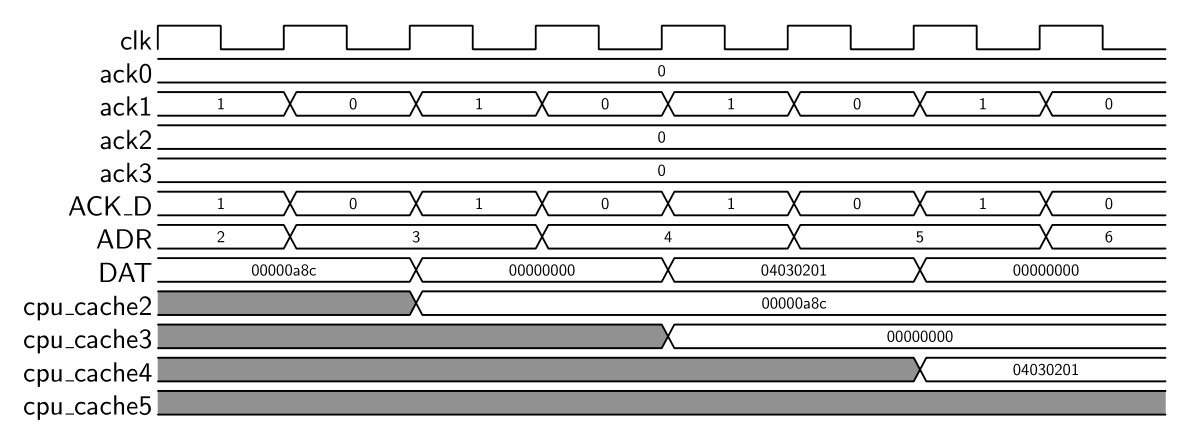
\includegraphics[width=\linewidth]{Chapitre4/figures/nofault1.png}
  \caption{Impact of acknowledge signal on address, data signals and CPU cache without attack}
  \label{nofault1}
\end{figure}

\begin{figure}[t!]
  \centering
  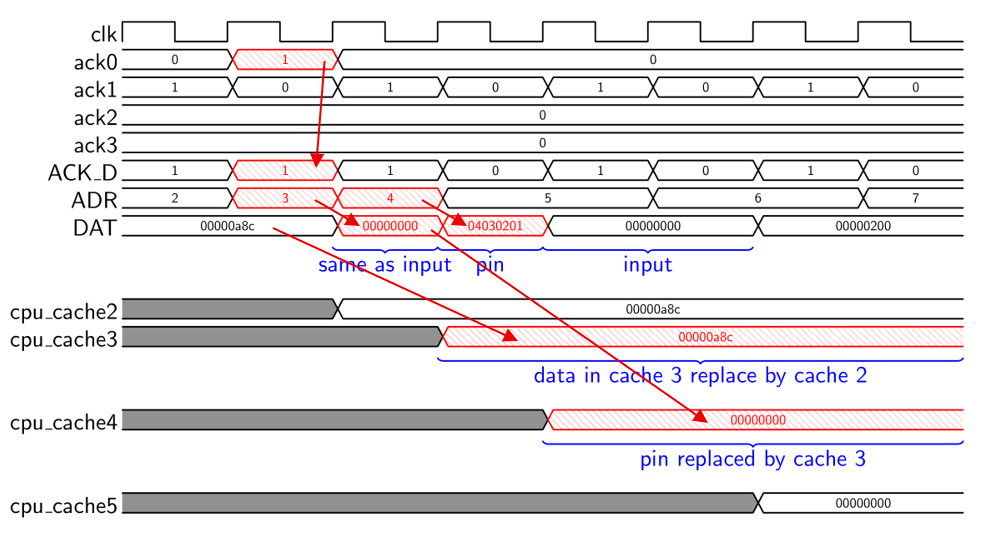
\includegraphics[width=\linewidth]{Chapitre4/figures/fault1.png}
  \caption{Impact of acknowledge signal on address, data signals and CPU cache with attack}
  \label{fault1}
\end{figure}

Next, we examine the impact of faults on the \texttt{grant} register. Figure~\ref{nofault2} depicts the expected behavior under normal operating conditions, with the clock waveform shown at the top. Initially, the \texttt{grant} register is set to 0, causing the CPU to fetch instruction values from the ROM. Starting from the second period, once the \texttt{grant} signal transitions to 1, the CPU begins accessing variable data stored in SRAM. The \texttt{ack1} signal, representing data acknowledge from the SRAM, alternates between "$0$" and "$1$" on each clock cycle, while the remaining \texttt{ACK} lines remain at "$0$". The global acknowledge signal \texttt{ACK\_D}, derived from \texttt{ack1}, orchestrates both the address increment (\texttt{ADR}) and data sampling (\texttt{DAT}), resulting in address and data updates occurring every two cycles.

During this process, the CPU retrieves the following sequence of data: 0x00000000, 0x04000000, and 0x10000018, located at addresses 0x7f0, 0x7f1, and 0x7f2, respectively. The content at 0x7f0 serves as the function code, while the first two bits at address 0x7f1 encode the size value, which is shared by both the card PIN and user PIN. The final value at 0x7f2 indicates the memory address pointing to the user's PIN. As in the previous case, each \texttt{DAT} value takes two cycles to propagate and is subsequently stored in cache addresses 0x1008, 0x1009, and 0x1010.

Figure~\ref{fault2} illustrates the behavior following a fault injection. A bit-flip is simultaneously introduced into both \texttt{ack0} and the \texttt{grant} register. The premature transition of \texttt{grant} causes the CPU to interpret control signals one cycle earlier than intended. Consequently, the acknowledge, address, and data signals all advance by one cycle. As in the previous scenario, this temporal shift in the \texttt{ACK} signal disrupts the timing of data reads. The third cache line mistakenly stores 0x0007c783 at cycle 3 in place of the correct 0x00000000, while the fourth cache line—intended to store the card PIN—incorrectly holds 0x00000000 instead of 0x04000000 at cycle 4. This leads to incorrect interpretation of the size value as zero, causing the loop body to execute zero times and thereby bypassing the authentication routine.

At the Register Transfer Level (RTL), a fault affecting the \texttt{grant} register may induce multiple bit-flips within the same cycle. From the perspective of instruction-level execution, such a fault can cause either premature or delayed signal responses. However, our current experimental observations indicate that faults targeting the \texttt{grant} register affect too many signals simultaneously, making it difficult to achieve precise fault effects. As such, isolated faults on \texttt{grant} have not yet resulted in successful exploitation within our current setup.

\begin{figure}[t!]
  \centering
  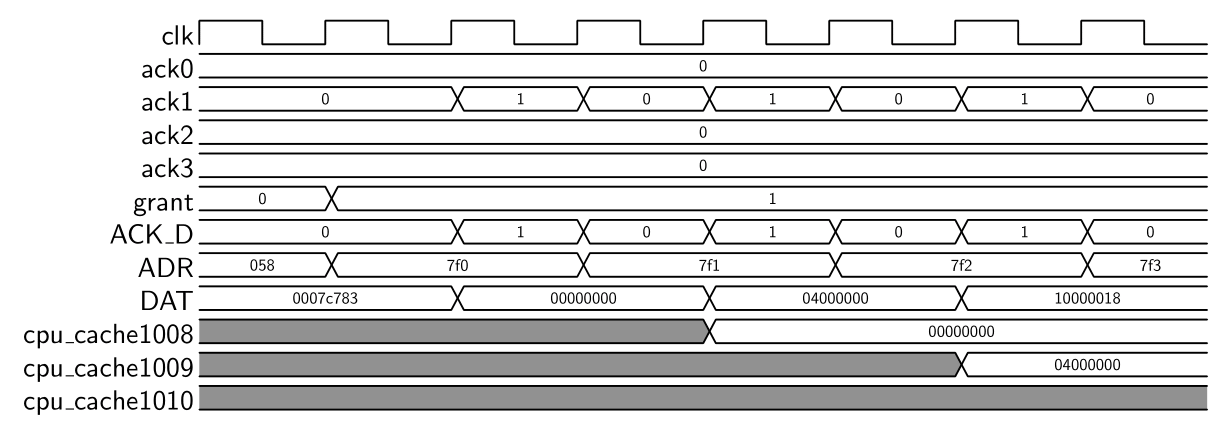
\includegraphics[width=\linewidth]{Chapitre4/figures/nofault2.png}
  \caption{Impact of grant signal on address, data signals and CPU cache without attack}
  \label{nofault2}
\end{figure}

\begin{figure}[t!]
  \centering
  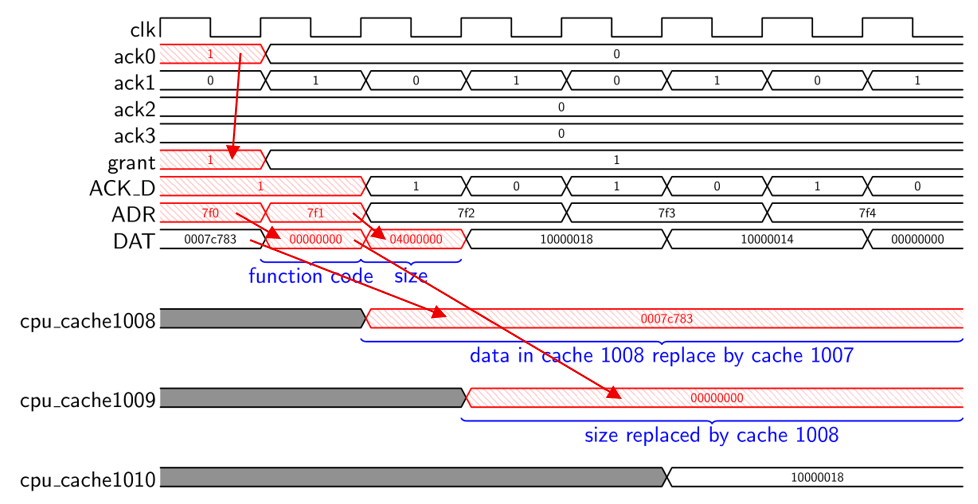
\includegraphics[width=\linewidth]{Chapitre4/figures/fault2.png}
  \caption{Impact of grant signal on address, data signals and CPU cache with attack}
  \label{fault2}
\end{figure}


The \texttt{SEL} register is vulnerable to various forms of fault injection. In the first attack scenario, referred to as data reset, the fault targets the data bus by manipulating the \texttt{SEL} signal. Under normal conditions—identical to those used in the \texttt{ACK} fault scenario—the CPU reads data from the SRAM, and the \texttt{SEL} register holds the value "0010". Each bit of the \texttt{SEL} signal is expanded to a 32-bit mask and then ANDed with the corresponding word in memory. In this case, the active selection results in SRAM data being masked with 0xffffffff, allowing the correct data to be transferred to the data bus.

However, if a fault occurs during the fifth cycle that forces the \texttt{SEL} register to "0000", each bit of the selection signal expands to 0x00000000. When ANDed with the corresponding memory data, this results in all selected words being zeroed. The four resulting 32-bit values (all 0x00000000) are then combined using a bitwise OR operation, yielding a final data word of 0x00000000. This corrupted value is then stored into the CPU cache.

When this fault takes place during the card PIN retrieval phase, the CPU ends up caching an all-zero value. If the user-provided PIN is also "0000", the comparison succeeds, resulting in unauthorized authentication. Notably, this attack achieves its effect by simultaneously resetting multiple bits of the \texttt{SEL} register, thereby masking the true contents of the data bus.

\begin{figure}[t!]
  \centering
  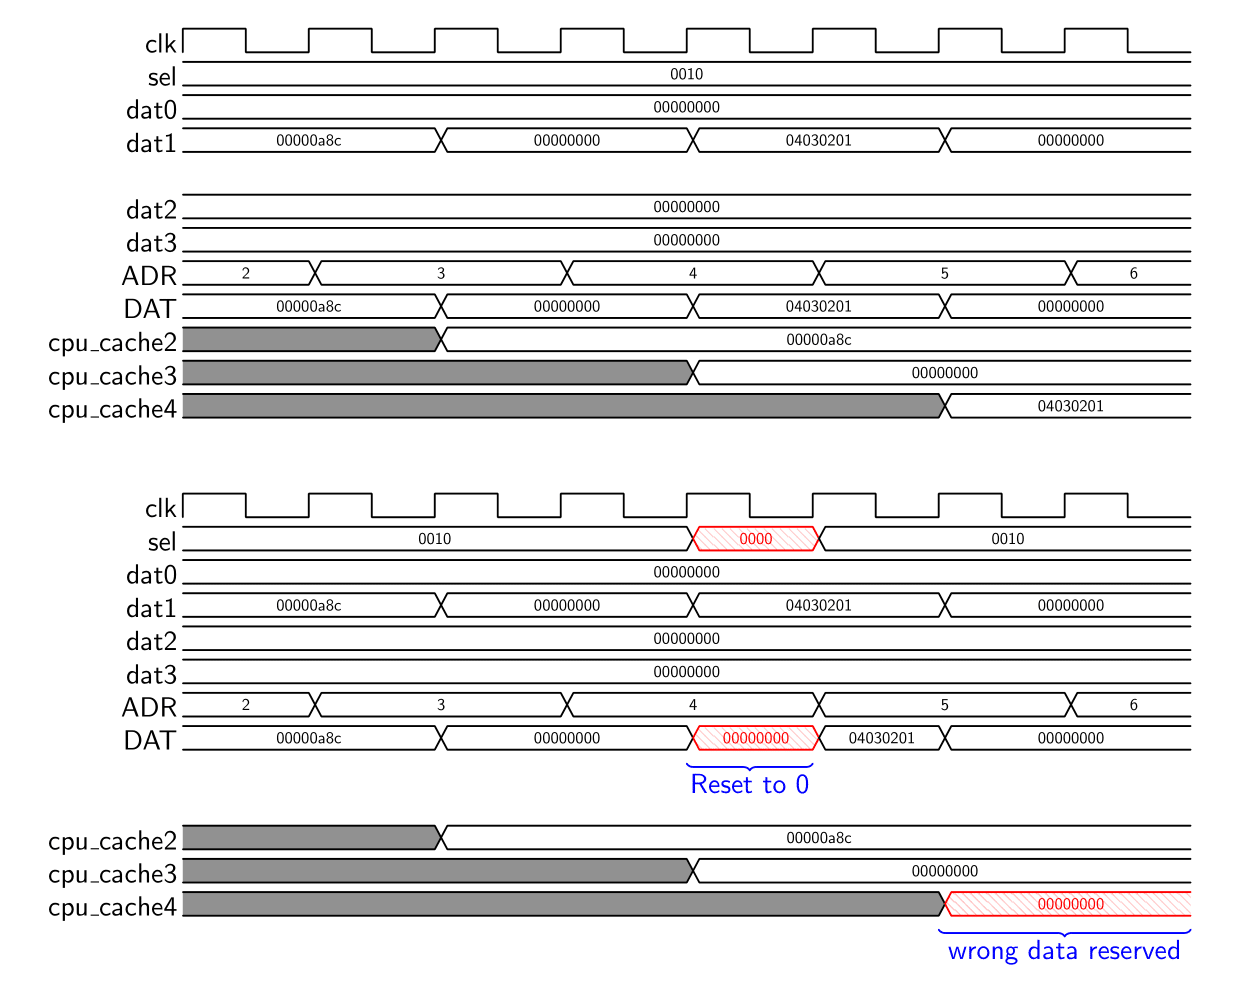
\includegraphics[width=\linewidth]{Chapitre4/figures/fault3.png}
  \caption{Impact of data reset on selection signal, data signals and CPU cache with/without attack}
  \label{fault3}
\end{figure}

In the second scenario, if a single unintended bit in the \texttt{SEL} register is set to "1" and the intended one is set to "0", this is called data misread. In our example as Figure \ref{fault4}, unlike SRAM is read in CPU in normal condition, ROM is read beacause of the attack on \texttt{SEL} register. In this case, the data "00000000" replace the correct card pin "04030201", cause the success.

\begin{figure}[t!]
  \centering
  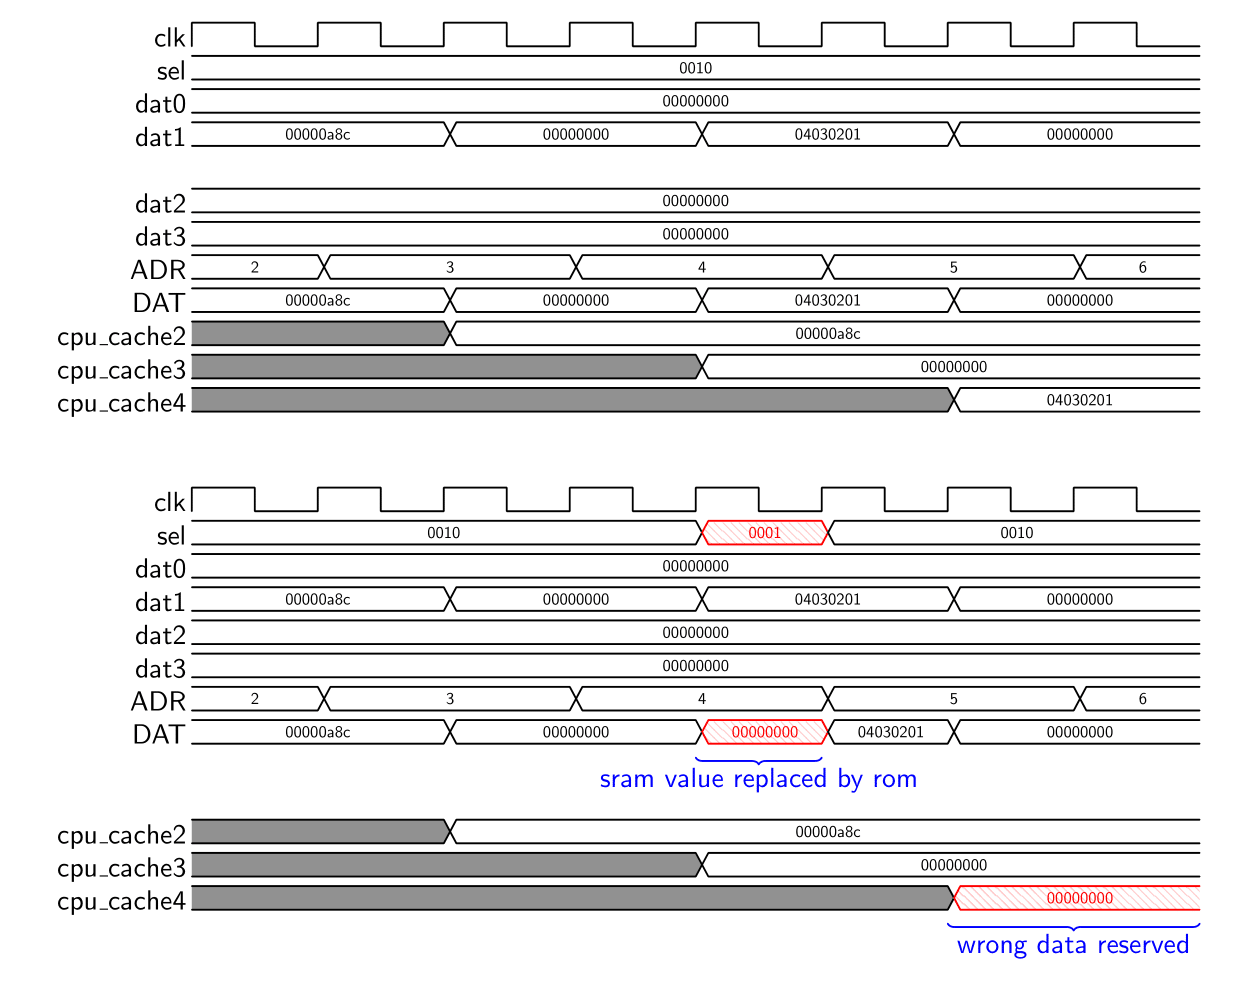
\includegraphics[width=\linewidth]{Chapitre4/figures/fault4.png}
  \caption{Impact of data misread on selection signal, data signals and CPU cache with/without attack}
  \label{fault4}
\end{figure}

In the third scenario, a fault causes more than one unintended bit in the \texttt{SEL} register to be set to "1", a condition referred to as data multiread. As shown in Figure~\ref{fault5}, the injected fault modifies \texttt{SEL} to "1100", resulting in both CSR and \texttt{MAIN\_RAM} being read by the CPU simultaneously. Since both memory regions were initialized with zero values, the data output from each is 0x00000000. The resulting \texttt{DAT} signal transmitted to the CPU is the bitwise OR of the two, which remains 0x00000000. This leads to a successful authentication bypass.

\begin{figure}[t!]
  \centering
  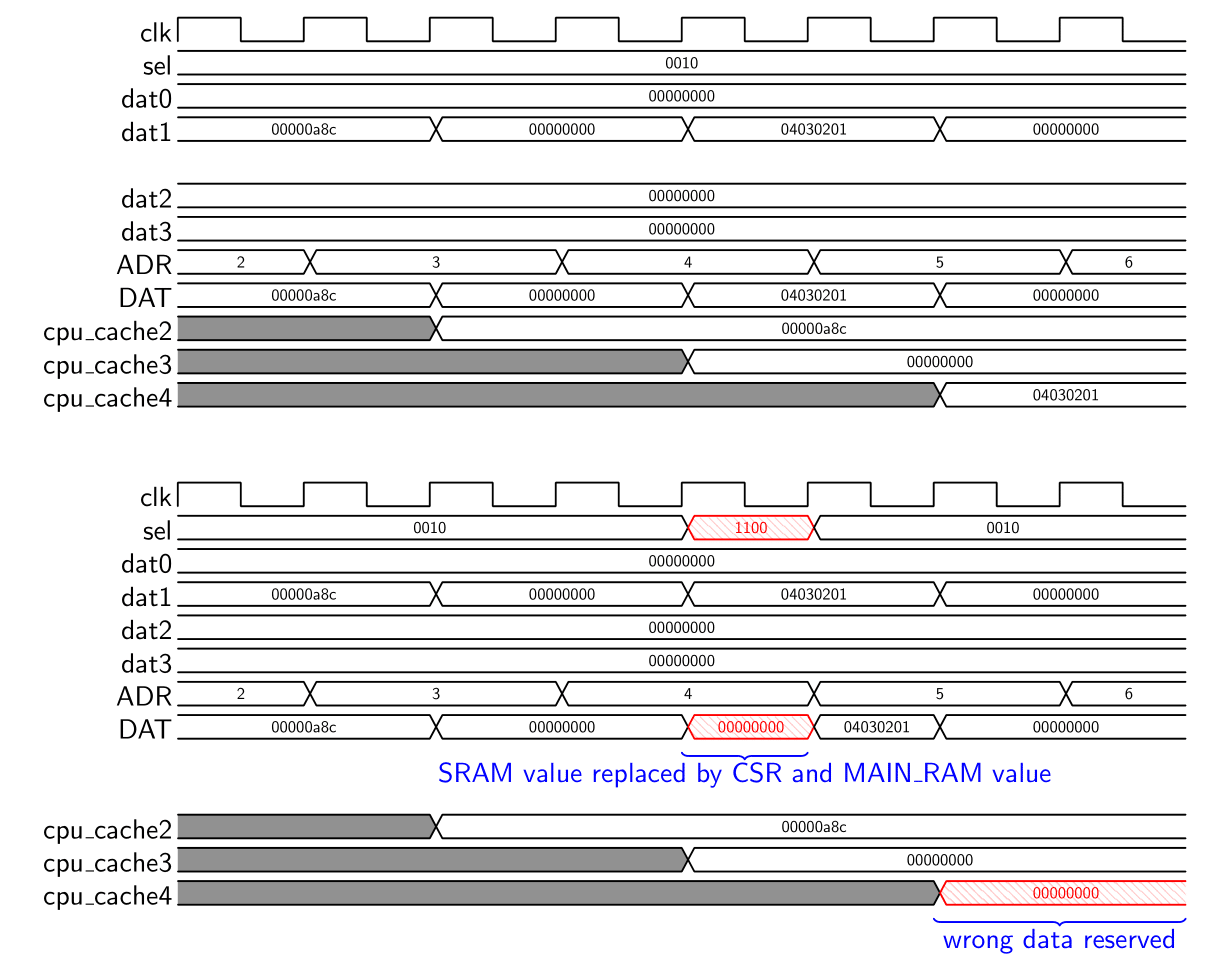
\includegraphics[width=\linewidth]{Chapitre4/figures/fault5.png}
  \caption{Impact of data multiread on selection signal, data signals and CPU cache with/without attack}
  \label{fault5}
\end{figure}

In general, attack on is \texttt{SEL} equivalent to multiple bit-resets/multiple bit-flips at RTL level and instruction replacement at instruction level. We can summarize two reasons for the success of the attack: the absence of a detector or corrector on the \texttt{ACK} and \texttt{SEL} signals; and the fact that the read bus does not use a multiplexer but a combinational logic gate. These disruptions demonstrate the critical impact of control signal vulnerabilities on the bus.

\begin{figure}[t!]
  \centering
  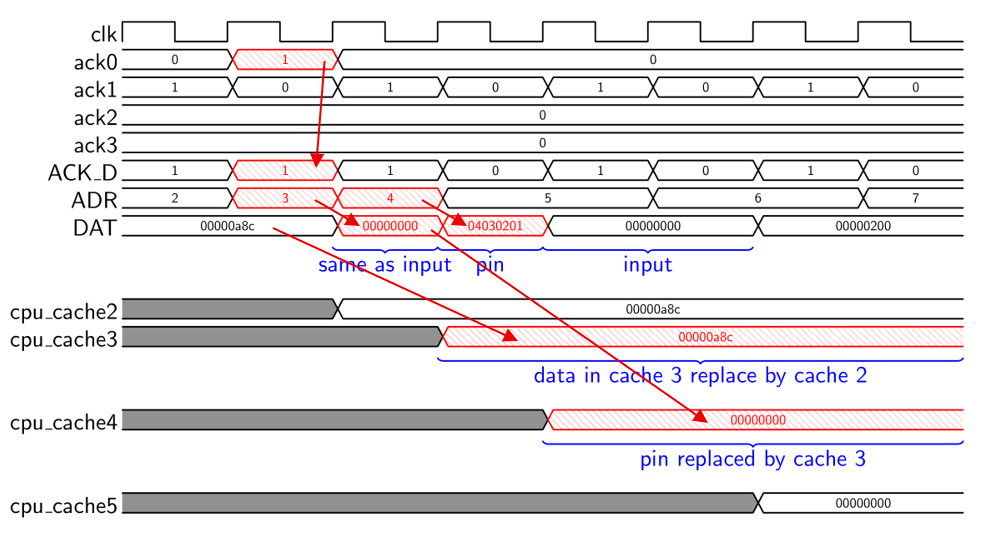
\includegraphics[width=\linewidth]{Chapitre4/figures/fault1.png}
  \caption{Impact of acknowledge signal on address, data signals and CPU cache without attack}
  \label{fault1}
\end{figure}

\begin{figure}[t!]
  \centering
  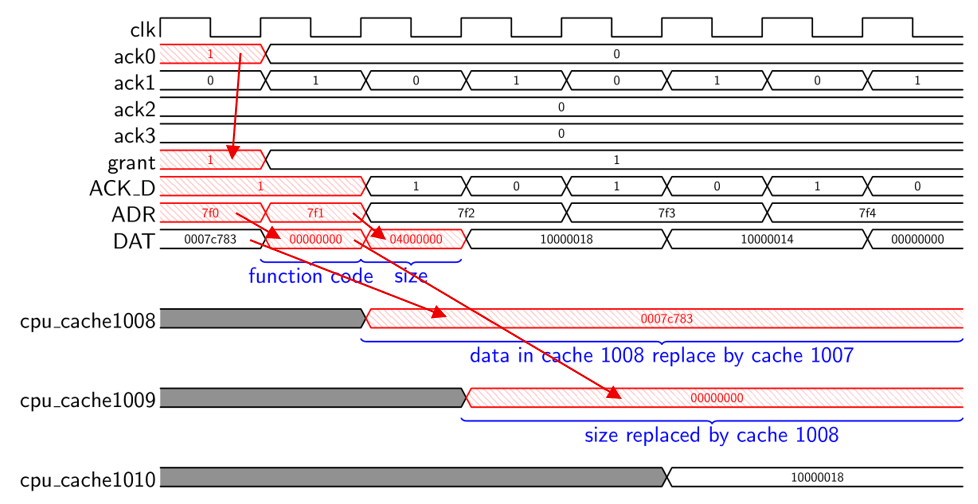
\includegraphics[width=\linewidth]{Chapitre4/figures/fault2.png}
  \caption{Impact of acknowledge signal on address, data signals and CPU cache with attack}
  \label{fault2}
\end{figure}

\section{Software countermeasures capacity against FIAs}

\subsection{Aim}
To effectively design countermeasures, we first analyze the sources and structures of vulnerability within the system. Our previous fault injection experiments reveal that attacks targeting the \texttt{ACK} and \texttt{SEL} signals can directly affect data flow integrity and control timing. These vulnerabilities arise from structural weaknesses: for instance, the absence of dedicated error detection or correction mechanisms on handshake and selection signals. Additionally, the \texttt{SEL} signal is controlled by a purely combinational multiplexer without any built-in verification logic. Such architectural choices leave the system particularly susceptible to fault injection that manipulates signal timing or selectively disables data paths, leading to corrupted reads and logical bypasses.

While implementing hardware-level countermeasures is possible, it often comes at a high resource cost, especially in lightweight embedded systems where logic and memory budget is constrained. In contrast, the existing \texttt{VerifyPin} benchmark already includes a software-level countermeasure designed to address software-based attacks, even though such attacks are outside the scope of this research. Nevertheless, these software countermeasures offer a valuable line of defense and can be extended to mitigate certain fault-induced vulnerabilities. Therefore, we choose to first implement a software-based countermeasure, as it provides a low-overhead solution compatible with the current system architecture and lays the foundation for evaluating integrated fault resilience.

\subsection{Countermeasure introduction}
The VerifyPin benchmark incorporate various countermeasures to enhance resilience against software attacks:

\begin{enumerate}
\item HB (Hardened Booleans): This technique encodes Boolean values using two constants with a high Hamming distance, making it more challenging to switch between values with a single fault injection. The primary objective is to protect against data-modifying faults.

\item FTL (Fixed-Time Loop): This countermeasure ensures that an algorithm's execution time remains constant regardless of the input data, thereby mitigating timing analysis attacks. By preventing variations in execution time, attackers are unable to infer sensitive information such as encryption keys. In the actual program, they implement this protection by verifying that the number of loops is correct.

\item INL (Inlined Functions): Function calls are replaced with their corresponding function code, reducing the attack surface. This countermeasure protects against instruction-skipping attacks on function calls by eliminating the instructions used to pass parameters during calls.

\item DPTC (PTC Decremented First): PTC refers to a counter used to regulate program loops or execution times. By decreasing the counter before entering critical code, the system prevents attackers from creating infinite loops or time exceptions through instruction skipping or unauthorized instruction insertion.

\item PTCBK (PTC Backup): This countermeasure safeguards against counter tampering or rollback attacks. By maintaining a backup of counter values, the system can revert to a trusted state if anomalies are detected. If the backup value differs from the current counter value, protective measures such as execution interruption can be triggered. In the actual program (V4), it copies the value of the counter to another variable, reduces the values of both and compares them to achieve this measure.

\item LC (Loop Counter): This mechanism monitors and limits the number of loop executions in a program to prevent infinite loops or excessive resource consumption. The system records the loop count during execution and triggers safety measures if the count exceeds predefined limits, thereby avoiding resource exhaustion or abnormal behavior.

\item DC (Double Call): To prevent tampering during critical function calls, the program executes two identical calls and compares their results. If the outcomes differ, the program identifies a potential attack or tampering attempt and may trigger protective responses.

\item DT (Double Test): This countermeasure ensures data integrity by performing two evaluations for key conditions. If the results differ, it indicates possible tampering, prompting the system to raise alarms or take protective measures.

\item SC (Step Counter): This technique monitors the number or sequence of critical program steps to prevent process control tampering. If the Step Counter deviates from the expected value, the system may abort execution or enter a protective mode to maintain operational security.
\end{enumerate}

As shown in Table~\ref{tab:benchmark cm}, A detailed explanation of each countermeasure is provided below.

\begin{table}
  \caption{Software countermeasures deployed in each benchmark version}
  \label{tab:benchmark cm}
  \begin{tabular}{cccccccccc}
    \hline
    & HB & FTL & INL & DPTC & PTCBK & LC & DC & DT & SC\\
    \hline
    \texttt{v0} & & & & & & & & &  \\
    \texttt{v1} & \checkmark & & & & & & & &  \\
    \texttt{v2} & \checkmark & \checkmark & & & & & & & \\
    \texttt{v3} & \checkmark & \checkmark & \checkmark & & & & & & \\
    \texttt{v4} & \checkmark & \checkmark & \checkmark & \checkmark & \checkmark & \checkmark & & &\\
    \texttt{v5} & \checkmark & \checkmark & & \checkmark & & & \checkmark & &  \\
    \texttt{v6} & \checkmark & \checkmark & \checkmark & \checkmark & & & & \checkmark &  \\
    \texttt{v7} & \checkmark & \checkmark & \checkmark & \checkmark & & & & \checkmark & \checkmark\\
    \hline
  \end{tabular}
\end{table}

In Figure\ref{V0}, we reuse the code.c file to show the countermeasure implement in other versions.
\begin{figure}
\begin{lstlisting}[caption={code.c of VerifyPin function in benchmark V0}, label={V0}, basicstyle=\ttfamily\footnotesize]
#include "interface.h"
#include "types.h"
#include "commons.h"

extern SBYTE g_ptc;
extern BOOL g_authenticated;
extern UBYTE g_userPin[PIN_SIZE];
extern UBYTE g_cardPin[PIN_SIZE];

#ifdef INLINE
__attribute__((always_inline)) inline BOOL byteArrayCompare(UBYTE* a1, UBYTE* a2, UBYTE size)
#else
BOOL byteArrayCompare(UBYTE* a1, UBYTE* a2, UBYTE size)
#endif
{
    int i;
    for(i = 0; i < size; i++) {
        if(a1[i] != a2[i]) {
            return 0;
        }
    }
    return 1;
}

BOOL verifyPIN() {
    g_authenticated = 0;

    if(g_ptc > 0) {
        if(byteArrayCompare(g_userPin, g_cardPin, PIN_SIZE) == 1) {
            g_ptc = 3;
            g_authenticated = 1; // Authentication();
            return 1;
        } else {
            g_ptc--;
            return 0;
        }
    }

    return 0;
}
\end{lstlisting}
\end{figure}

In Version 1 Figure\ref{V1}, the HB countermeasure is implemented at lines 19 and 22. We replace the original return values 0 and 1 with the Boolean constants false and true. This modification allows us to verify whether the variable comp is altered to any unexpected value outside the Boolean domain. By doing so, we can detect potential fault attacks that attempt to manipulate comp to bypass verification logic.

\begin{figure}
\begin{lstlisting}[caption={code.c of VerifyPin function in benchmark V1}, label={V1}, basicstyle=\ttfamily\footnotesize]
#include "interface.h"
#include "types.h"
#include "commons.h"

extern SBYTE g_ptc;
extern BOOL g_authenticated;
extern UBYTE g_userPin[PIN_SIZE];
extern UBYTE g_cardPin[PIN_SIZE];

#ifdef INLINE
 __attribute__((always_inline)) inline BOOL byteArrayCompare(UBYTE* a1, UBYTE* a2, UBYTE size)
#else
BOOL byteArrayCompare(UBYTE* a1, UBYTE* a2, UBYTE size)
#endif
{
    int i;
    for(i = 0; i < size; i++) {
        if(a1[i] != a2[i]) {
            return BOOL_FALSE;
        }
    }
    return BOOL_TRUE;
}

BOOL verifyPIN() {
    int comp;
    g_authenticated = BOOL_FALSE;

    if(g_ptc > 0) {
        comp = byteArrayCompare(g_userPin, g_cardPin, PIN_SIZE);
        if(comp == BOOL_TRUE) {
            g_ptc = 3;
            g_authenticated = BOOL_TRUE; // Authentication();
            return BOOL_TRUE;
        } else if(comp == BOOL_FALSE) {
          g_ptc--;
          return BOOL_FALSE;
        } else {
          countermeasure();
        }
    }
    return BOOL_FALSE;
}
\end{lstlisting}
\end{figure}

In Version 2 (Figure \ref{V2}), the HB countermeasure is implemented in the same way as in Version 1. In addition to this, FTL protection is introduced. Specifically, after the loop concludes, a check is performed at line 25 to verify whether the loop counter has reached the expected value. This serves to detect any premature termination of the loop that could be caused by a fault injection attack.

\begin{figure}
\begin{lstlisting}[caption={code.c of VerifyPin function in benchmark V2}, label={V2}, basicstyle=\ttfamily\footnotesize]
#include "interface.h"
#include "types.h"
#include "commons.h"

extern SBYTE g_ptc;
extern BOOL g_authenticated;
extern UBYTE g_userPin[PIN_SIZE];
extern UBYTE g_cardPin[PIN_SIZE];
extern UBYTE g_countermeasure;

#ifdef LAZART
  __attribute__((always_inline)) inline BOOL byteArrayCompare(UBYTE* a1, UBYTE* a2, UBYTE size)
#else
  BOOL byteArrayCompare(UBYTE* a1, UBYTE* a2, UBYTE size)
#endif
{
    int i;
    BOOL status = BOOL_FALSE;
    BOOL diff = BOOL_FALSE;
    for(i = 0; i < size; i++) {
        if(a1[i] != a2[i]) {
            diff = BOOL_TRUE;
        }
    }
    if(i != size) {
        countermeasure();
    }
    if (diff == BOOL_FALSE) {
        status = BOOL_TRUE;
    } else {
        status = BOOL_FALSE;
    }

    return status;
}

BOOL verifyPIN()
{
    g_authenticated = BOOL_FALSE;

    if(g_ptc > 0) {
        if(byteArrayCompare(g_userPin, g_cardPin, PIN_SIZE) == BOOL_TRUE) {
            g_ptc = 3;
            g_authenticated = BOOL_TRUE; // Authentication();
            return BOOL_TRUE;
        } else {

            g_ptc--;
            return BOOL_FALSE;
        }
    }
    return BOOL_FALSE;
}
\end{lstlisting}
\end{figure}

In Version 3 (Figure \ref{V3}), both the HB and FTL countermeasures are implemented identically to Version 2. In addition to these, INL protection is introduced. Specifically, at line 33, instead of invoking the byteArrayCompare function, the comparison logic is written directly within the same function. This modification is intended to eliminate potential vulnerabilities that may arise during function calls, such as control-flow manipulation or return address corruption due to fault injection.

\begin{figure}
\begin{lstlisting}[caption={code.c of VerifyPin function in benchmark V3}, label={V3}, basicstyle=\ttfamily\footnotesize]
#include "interface.h"
#include "types.h"
#include "commons.h"

extern SBYTE g_ptc;
extern BOOL g_authenticated;
extern UBYTE g_userPin[PIN_SIZE];
extern UBYTE g_cardPin[PIN_SIZE];

BOOL verifyPIN() {
    int i;
    BOOL status;
    BOOL diff;
    g_authenticated = BOOL_FALSE;

    if(g_ptc > 0) {
        status = BOOL_FALSE;
        diff = BOOL_FALSE;
        for(i = 0; i < PIN_SIZE; i++) {
            if(g_userPin[i] != g_cardPin[i]) {
                diff = BOOL_TRUE;
            }
        }
        if(i != PIN_SIZE) {
            countermeasure();
        }
        if (diff == BOOL_FALSE) {
            status = BOOL_TRUE;
        } else {
            status = BOOL_FALSE;
        }

        if(status == BOOL_TRUE) {
            g_ptc = 3;
            g_authenticated = BOOL_TRUE; // Authentication();
            return BOOL_TRUE;
        } else {
            g_ptc--;
            return BOOL_FALSE;
        }
    }
    return BOOL_FALSE;
}
\end{lstlisting}
\end{figure}

In Version 4 (Figure \ref{V4}), the HB, FTL, and INL countermeasures are implemented in the same manner as in Version 2. In addition to these, three new protections are introduced: DPTC, PTCBK, and LC. Specifically, at line 22, the variable g\_ptc is decremented to help restore the system to a consistent internal state, thereby mitigating potential inconsistencies caused by an attack. At line 15, the value of g\_ptc is copied into a temporary variable ptcCpy, which is later checked to detect any unauthorized modifications, preventing tampering with the control variable. Finally, at line 35, a stepCounter variable is used to track the number of loop iterations, helping to detect and prevent control-flow faults that might cause the loop to be skipped or prematurely terminated.

\begin{figure}
\begin{lstlisting}[caption={code.c of VerifyPin function in benchmark V4}, label={V4}, basicstyle=\ttfamily\footnotesize]
#include "interface.h"
#include "types.h"
#include "commons.h"

extern SBYTE g_ptc;
extern BOOL g_authenticated;
extern UBYTE g_userPin[PIN_SIZE];
extern UBYTE g_cardPin[PIN_SIZE];

BOOL verifyPIN() {
    int i;
    BOOL status;
    BOOL diff;
    int stepCounter;
    SBYTE ptcCpy = g_ptc;
    g_authenticated = BOOL_FALSE;

    if(g_ptc > 0) {
        if(ptcCpy != g_ptc) {
            countermeasure();
        }
        g_ptc--;
        if(g_ptc != ptcCpy-1) {
            countermeasure();
        }
        ptcCpy--;

        status = BOOL_FALSE;
        diff = BOOL_FALSE;
        stepCounter = 0;
        for(i = 0; i < PIN_SIZE; i++) {
            if(g_userPin[i] != g_cardPin[i]) {
                diff = BOOL_TRUE;
            }
            stepCounter++;
        }
        if(stepCounter != PIN_SIZE) {
            countermeasure();
        }
        if(i != PIN_SIZE) {
            countermeasure();
        }
        if (diff == BOOL_FALSE) {
            status = BOOL_TRUE;
        } else {
            status = BOOL_FALSE;
        }

        if(status == BOOL_TRUE) {
            if(ptcCpy != g_ptc) {
                countermeasure();
            }
            g_ptc = 3;
            g_authenticated = BOOL_TRUE; // Authentication();
            return BOOL_TRUE;
        }
    }

    return BOOL_FALSE;
}
\end{lstlisting}
\end{figure}

In Version 5 (Figure \ref{V5}), DC protection is introduced. Specifically, at line 42, the byteArrayCompare function is called twice consecutively to obtain two results. This redundancy helps to detect and prevent fault injection attacks targeting the function call itself.

\begin{figure}
\begin{lstlisting}[caption={code.c of VerifyPin function in benchmark V5}, label={V5}, basicstyle=\ttfamily\footnotesize]
#include "interface.h"
#include "types.h"
#include "commons.h"

extern SBYTE g_ptc;
extern BOOL g_authenticated;
extern UBYTE g_userPin[PIN_SIZE];
extern UBYTE g_cardPin[PIN_SIZE];

#ifdef INLINE
__attribute__((always_inline)) inline BOOL byteArrayCompare(UBYTE* a1, UBYTE* a2, UBYTE size)
#else
BOOL byteArrayCompare(UBYTE* a1, UBYTE* a2, UBYTE size)
#endif
{
    int i;
    BOOL status = BOOL_FALSE;
    BOOL diff = BOOL_FALSE;
    for(i = 0; i < size; i++) {
        if(a1[i] != a2[i]) {
            diff = BOOL_TRUE;
        }
    }
    if(i != size) {
        countermeasure();
    }
    if (diff == BOOL_FALSE) {
        status = BOOL_TRUE;
    } else {
        status = BOOL_FALSE;
    }
    return status;
}

BOOL verifyPIN() {
    g_authenticated = BOOL_FALSE;

    if(g_ptc > 0) {
        g_ptc--;

        if(byteArrayCompare(g_userPin, g_cardPin, PIN_SIZE) == BOOL_TRUE) {
            if(byteArrayCompare(g_cardPin, g_userPin, PIN_SIZE) == BOOL_TRUE) {
                g_ptc = 3;
                g_authenticated = BOOL_TRUE; // Authentication();
                return BOOL_TRUE;
            } else countermeasure();
        }
    }

    return BOOL_FALSE;
}
\end{lstlisting}
\end{figure}

In Version 6 (Figure \ref{V6}), DT protection is implemented. Specifically, at lines 30 and 40, the values diff and status are compared twice consecutively to detect and prevent fault injection attacks targeting the comparison operations.

\begin{figure}
\begin{lstlisting}[caption={code.c of VerifyPin function in benchmark V6}, label={V6}, basicstyle=\ttfamily\footnotesize]
#include "interface.h"
#include "types.h"
#include "commons.h"

extern SBYTE g_ptc;
extern BOOL g_authenticated;
extern UBYTE g_userPin[PIN_SIZE];
extern UBYTE g_cardPin[PIN_SIZE];

BOOL verifyPIN() {
    int i;
    BOOL status;
    BOOL diff;
    g_authenticated = BOOL_FALSE;

    if(g_ptc > 0) {
        g_ptc--;

        status = BOOL_FALSE;
        diff = BOOL_FALSE;
        for(i = 0; i < PIN_SIZE; i++) {
            if(g_userPin[i] != g_cardPin[i]) {
                diff = BOOL_TRUE;
            }
        }
        if(i != PIN_SIZE) {
            countermeasure();
        }
        if (diff == BOOL_FALSE) {
            if(BOOL_FALSE == diff) {
                status = BOOL_TRUE;
            } else {
                countermeasure();
            }
        } else {
            status = BOOL_FALSE;
        }

        if(status == BOOL_TRUE) {
            if(BOOL_TRUE == status) {
                g_ptc = 3;
                g_authenticated = BOOL_TRUE; // Authentication();
                return BOOL_TRUE;
            } else {
                countermeasure();
            }
        }
    }

    return BOOL_FALSE;
}
\end{lstlisting}
\end{figure}

In Version 7 (Figure \ref{V7}), SC protection is implemented. Specifically, a variable stepCounter is used to track the number of executed actions. After execution, the value of stepCounter is verified to ensure correctness. This mechanism effectively mitigates nearly all types of instruction skip attacks occurring at the line level.

\begin{figure}
\begin{lstlisting}[caption={code.c of VerifyPin function in benchmark V7}, label={V7}, basicstyle=\ttfamily\footnotesize]
#include "interface.h"
#include "types.h"
#include "commons.h"

extern SBYTE g_ptc;
extern BOOL g_authenticated;
extern UBYTE g_userPin[PIN_SIZE];
extern UBYTE g_cardPin[PIN_SIZE];

BOOL verifyPIN() {
    int stepCounter = 0;
    int i;
    BOOL status;
    BOOL diff;
    g_authenticated = BOOL_FALSE;

    if(g_ptc > 0) {
        stepCounter++;
        if(stepCounter != 1) {
            countermeasure();
        }
        g_ptc--;
        stepCounter++;
        if(stepCounter != 2) {
            countermeasure();
        }

        status = BOOL_FALSE;
        diff = BOOL_FALSE;

        stepCounter++;
        if(stepCounter != 3) {
            countermeasure();
        }

        for(i = 0; i < PIN_SIZE; i++) {
            if(g_userPin[i] != g_cardPin[i]) {
                diff = BOOL_TRUE;
            }
            stepCounter++;
            if(stepCounter != i+4) {
                countermeasure();
            }
        }
        stepCounter++;
        if(stepCounter != 4+PIN_SIZE) {
            countermeasure();
        }
        if(i != PIN_SIZE) {
            countermeasure();
        }
        if (diff == BOOL_FALSE) {
            if(BOOL_FALSE == diff) {
                status = BOOL_TRUE;
            } else {
                countermeasure();
            }
        } else {
            status = BOOL_FALSE;
        }
        stepCounter++;
        if(stepCounter != 5+PIN_SIZE) {
            countermeasure();
        }

        if(status == BOOL_TRUE) {
            stepCounter++;
            if(stepCounter != 6+PIN_SIZE) {
                countermeasure();
            }
            if(BOOL_TRUE == status) {
                stepCounter++;
                if(stepCounter != 7+PIN_SIZE) {
                    countermeasure();
                }
                g_ptc = 3;
                stepCounter++;
                if(stepCounter != 8+PIN_SIZE) {
                    countermeasure();
                }
                g_authenticated = BOOL_TRUE; // Authentication();
                return BOOL_TRUE;
            } else {
                countermeasure();
            }
        } else {
            countermeasure();
        }
    }

    return BOOL_FALSE;
}
\end{lstlisting}
\end{figure}

\subsection{Step}
To initialize the formal verification process, we compile multiple versions of the VerifyPin benchmark (from V1 to V7) into formal model files. Throughout this process, the system configuration remains consistent with the previous setup, particularly regarding the Wishbone bus integration. Based on these settings, we proceed to generate the corresponding SoC in the form of a Verilog project, ensuring functional consistency and compatibility across all versions.

For automated fault injection, we utilize the FISSA framework. The target registers for injection are kept unchanged, as no structural modifications have been made to the architecture itself. However, due to the increasing complexity and size of the application—especially after incorporating software countermeasures—we update the parameters \texttt{fenetre\_tir} and \texttt{cycle\_ref} within the configuration file \texttt{config\_wop.json}. Additionally, the comparison threshold against the variable \texttt{now} in the script \texttt{fault\_injection.py} is adjusted accordingly to align with the extended execution timeline of the newer program versions.

These configuration changes are summarized in Table~\ref{tab:variable configuration}, reflecting the necessary adjustments made to accommodate the increased program footprint and ensure consistent fault injection behavior across all benchmark iterations.

\begin{table}[]
  \caption{Difference in variable configuration in different version}
  \label{tab:variable configuration}
\begin{tabular}{rrrrr}
\multicolumn{1}{l}{version} & \multicolumn{1}{l}{from(fenetre\_tir)} & \multicolumn{1}{l}{to(fenetre\_tir)} & \multicolumn{1}{l}{threshold} & \multicolumn{1}{l}{cycle\_ref} \\
1 & 15870 & 18190 & 18264 & 2283 \\
2 & 15726 & 19390 & 19464 & 2433 \\
3 & 15694 & 18838 & 18912 & 2364 \\
4 & 15726 & 19918 & 19992 & 2499 \\
5 & 15678 & 19166 & 19240 & 2405 \\
6 & 15806 & 19014 & 19088 & 2386 \\
7 & 6062 & 14486 & 15504 & 1938
\end{tabular}
\end{table}

Because we add countermeasure, we change simulation results classification:
\begin{enumerate}
\item Crash, the simulation either exceeded the fixed execution time or triggered a crash signal, resulting in termination.
\item Detect, the fault was detected by the countermeasure, setting the variable \texttt{g\_countermeasure} to "1".
\item Success, the authentication bypassed successfully, with \texttt{g\_authenticated} set to "1".
\item Change, no successful authentication or detection occurred, but the memory state was altered by the fault.
\item Silence, no authentication success, detection, or memory state change was observed, indicating the fault had no visible impact.
\end{enumerate}

In parallel with the robustness testing of different benchmark versions, we employed the \texttt{Lizard} tool~\cite{Lizard} to analyze their code complexity and computational cost. The complexity metrics for each benchmark are presented in Table~\ref{tab:benchmark result}. \texttt{Lizard} provides a detailed analysis across various parameters, which are described as follows:
\begin{enumerate}
\item NLOC (Non-Commenting Lines of Code): This metric represents the total number of valid lines of code, excluding blank lines and comments. It serves as a direct indicator of code size and readability.

\item CCN (Cyclomatic Complexity Number): This metric measures the McCabe complexity of all functions, which reflects the number of independent logical paths within a program. Higher CCN values indicate greater logical complexity, making the code more challenging to maintain and test.

\item Token Count: This parameter represents the total number of lexical units, including operators, operands, and other functional elements. It provides insight into the syntactic complexity of the program.
\end{enumerate}

We install the \texttt{Lizard} analysis tool on a Linux-based system to evaluate code complexity metrics across different versions of the \texttt{VerifyPin} benchmark. For each version, \texttt{Lizard} is executed within the corresponding source directory. This process allows us to extract key software metrics such as function count, cyclomatic complexity, and lines of code, which are later used for comparative analysis. The extracted elements are consistent with those previously defined.

\subsection{Result}

The experimental results validate the initial hypothesis that the vulnerabilities are primarily concentrated on the \texttt{ACK}, \texttt{grant} and \texttt{SEL} signals. A detailed evaluation of the condition numbers is presented in Table~\ref{tab:benchmark result}. Among the eight benchmark versions, V7 exhibited the lowest fault injection success rate, whereas V4 achieved the highest fault detection capability. Further examination revealed a notable relationship between the complexity of the countermeasures—measured by code length, cyclomatic complexity (CCN), and token count—and the total number of required simulation cycles. As the countermeasures became more elaborate, program execution time increased, inadvertently expanding the fault injection surface.

Interestingly, certain countermeasures that lacked alignment with the specific characteristics of the fault model—failing to effectively intercept or neutralize relevant fault paths—produced higher success rates than even the baseline versions without protection, such as V1 and V5. This counterintuitive outcome implies that while the fundamental fault model remained consistent, none of the implemented countermeasures succeeded in fully neutralizing the fault impact. These findings highlight the necessity for a more granular analysis of each countermeasure’s logic and deployment in order to uncover the underlying reasons behind this anomalous behavior.

\begin{table*}
  \centering
  \caption{Fault injection results and code complexity metrics for each benchmark version}
  \label{tab:benchmark result}
\begin{tabular}{ccccccccccc}
\hline
& crash & detect & success & change & silence & success rate & sum & NLOC & CCN & token \\
\hline
V0 & 43 & 0 & 24 & 69 & 2438 & 0.93\% & 2574 & 32 & 6 & 107 \\
V1 & 68 & 19 & 37 & 103 & 2963 & 1.16\% & 3190 & 36 & 7 & 127 \\
V2 & 88 & 16 & 50 & 124 & 4760 & 0.99\% & 5038 & 44 & 8 & 149 \\
V3 & 81 & 23 & 15 & 109 & 4095 & 0.35\% & 4323 & 32 & 7 & 129 \\
V4 & 94 & 125 & 17 & 88 & 5440 & 0.29\% & 5764 & 47 & 11 & 191 \\
V5 & 92 & 27 & 39 & 114 & 4524 & 0.81\% & 4796 & 42 & 9 & 163 \\
V6 & 78 & 22 & 10 & 97 & 4204 & 0.23\%  & 4411 & 38 & 9 & 153 \\
V7 & 110 & 200 & 5 & 99 & 9673 & 0.05\% & 10087 & 77 & 18 & 312\\       
\hline                          
\end{tabular}
\end{table*}

\begin{table*}
  \centering
  \caption{Skipped instructions caused by attacks in V0, V1, V4, and V5 benchmarks}
  \label{tab:fault analysis}
\resizebox{\textwidth}{!}{%
\begin{tabular}{llllcc}
    \hline
& skipped instruction & code correct & code corrupt & code line & new fault \\
    \hline
& li a5, 1 & if(function == 1) & if(function == \textcolor{red}{0}) & 10 &\\
& bne a4, a5, loc\_1FC & if(function == 1) & jump to \textcolor{red}{ g\_authenticated = 1} & 10 &\\
& lbu a5, 20h+size(sp) & if (i \textless size) & if (i \textless \textcolor{red}{ i}) & 2 &\\
\multirow{-4}{*}{V0} & li a5, 0 & return 0 & return \textcolor{red}{ 1} & 3 &\\
\hline

& li a5, 1 & if(comp == 1) & if(comp == \textcolor{red}{ 0}) & 11 &\\
& bne a4, a5, loc\_200 & if(comp == 1) & jump to \textcolor{red}{ g\_authenticated = 1} & 11 &\\
& mv a5, a2 & store size value as 4 & store size value as \textcolor{red}{0} & 1 & \checkmark\\
& sb a5, 20h+size(sp) & store size value as 4 & store size value as \textcolor{red}{ random} & 1 & \checkmark\\
& li a5, 0 & return 0 & return \textcolor{red}{ 1} & 3 &\\
& j loc\_18C & jump to return 0 & jump to \color[HTML]{FF0000} {next loop} & 3 & \checkmark\\
& lbu a5, 20h+size(sp) & if (i \textless size) & if (i \textless \textcolor{red}{ i}) & 2 &\\
\multirow{-8}{*}{V1} & sw a5, 1Ch+comp(sp) & comp = 0 & comp =\textcolor{red}{ random} & 10 & \checkmark\\
\hline

& sb a5, 1Ch+diff(sp) & diff = 1 & diff = \textcolor{red}{ random} & 12 & \\
& bnez a5, loc\_258 & if (diff == 0) & jump to \textcolor{red}{ status = 1} & 16 &\\      
\multirow{-3}{*}{V4} & bne a4, a5, loc\_29C & if (status = 1) & jump to \textcolor{red}{ g\_authenticated = 1} & 18 &\\
\hline

& mv a5, a2 & store size value as 4 & store size value as \textcolor{red}{ random} & 1 & \checkmark\\
& sb a5, 2Ch+size(sp) & store size value as 4 & store size value as \textcolor{red}{ 0} & 1 & \checkmark\\
& lbu a5, 2Ch+size(sp) & if (i \textless size) & if (i \textless \textcolor{red}{ i}) & 4 & \checkmark\\
& sb a5, 2Ch+diff(sp) & diff = 1 & diff = \textcolor{red}{ random} & 5 &\\
& bnez a5, loc\_1B8 & if (diff == 0) &  jump to \textcolor{red}{ status = 1} & 8 &\\
& sb zero, 2Ch+status(sp) & status = 0 & status = \textcolor{red}{ random} & 9 & \checkmark\\
\multirow{-7}{*}{V5} & lbu a5, 2Ch+status(sp) & status = 0 & status = \textcolor{red}{ 1} & 9 & \checkmark\\ 
\hline
\end{tabular}
}
\end{table*}

Across all benchmark versions, successful fault injections were observed to impact both data signals originating from SRAM and instruction signals sourced from ROM. As previously discussed, data-related vulnerabilities are primarily induced by faults on the \texttt{ACK} and \texttt{SEL} signals. However, given that the frequency of successful data attacks remains largely consistent across all versions, these do not appear to be the dominant contributors to the observed differences in attack success rates.

In comparison, instruction-level vulnerabilities exert a more substantial influence. These faults are predominantly associated with "skip-repeat" behavior triggered by instruction-level disruptions—most notably, those induced by \texttt{ACK} faults. Since many repeated instructions (e.g., arithmetic, logical, and comparison operations) are inherently idempotent, their unintended repetition often leaves program behavior unchanged. The more critical consequence arises from instruction skipping, which more significantly compromises program integrity and thus increases the likelihood of attack success.

A comprehensive overview of all identified fault vulnerabilities is provided in Table~\ref{tab:fault analysis}. This includes the relevant assembly sequences used in fault payloads, associated code fragments, the specific code locations where the faults manifest, and an indication of whether each vulnerability was previously known or newly identified in this work.

From V0 (Listing~\ref{V0}) to V1 (Listing~\ref{V1}), a hardened Boolean countermeasure was introduced to protect the result of the function that compares the user PIN and the card PIN from being easily manipulated (V1 lines 19). This countermeasure mitigates attacks that exploit instruction skipping on the else branch. However, attacks that skip the comparison condition—\texttt{if(function == 1)} (V0 line 29) and \texttt{if(comp == 1)} (V1 line 31)—remain undetected. Additionally, faults such as skipping instructions responsible for reading constant values (line 17 in V0 and in V1), the variable \texttt{size} (line 13 in V0 and in V1), or the return value (line 19 in V0 and V1) are not protected and remain exploitable. Furthermore, the increased instruction count in V1 introduces new vulnerable locations (marked as "new fault" in Table \ref{tab:fault analysis}), creating additional fault injection opportunities. As a result, the attack success rate in V1 unexpectedly increases rather than decreases.

A similar trend is observed when comparing V4 in Listing~\ref{V4} to V5 in Listing~\ref{V5}. In V5, three countermeasures — backup counter value, inlined calls and loop counter (V4 lines 22, 31, 35)  — were removed, while a new countermeasure, double call, was introduced in line 33. The removal of the loop counter eliminated protection on the loop counter variable, which allows fault injection to manipulate the statement \texttt{if (i < size)}(V5 line 19). It controls loop iterations, potentially forcing premature loop termination. The exclusion of inlined calls increased the instruction count for reading the variables \texttt{size} and \texttt{status}, exposing these operations to instruction-skipping attacks that assign unintended random values. Although the backup counter value on variable \texttt{g\_ptc} was removed, this did not affect the attack success rate since no attacks were observed targeting \texttt{g\_ptc}. Notably, while V4 was vulnerable to attacks on the code \texttt{if(status == true)} in line 49, the introduction of the double call countermeasure in V5 successfully mitigated similar attacks on the corresponding instruction. However, the code \texttt{diff = true} (V4 line 33, V5 line 21) and \texttt{if(diff == false)} (V4 line 43, V5 line 27) remained unprotected across both versions, leaving them vulnerable to fault injection attacks. Overall, the changes in countermeasures introduced more vulnerabilities than they mitigated, resulting in a higher attack success rate in V5.

A comparative evaluation of the countermeasures applied against hardware-induced faults targeting protected instructions is presented in Table~\ref{tab:cm evaluate}. Our experimental findings indicate that the implemented protections—\texttt{INL}, \texttt{LC}, \texttt{DC}, \texttt{DT}, and \texttt{SC}—when applied to critical operations such as comparison checks and loop control, are generally effective in addressing instruction-level vulnerabilities characterized by the skip-repeat fault model.

Nonetheless, it is crucial to recognize that the observed effectiveness is influenced by the nature of the test programs and the specific deployment of each countermeasure. A method that appeared less effective in our benchmarks might yield better results if repositioned or more tightly integrated within different code structures. Moreover, since these software-based defenses function at the instruction granularity, while hardware faults—even when modeled as single bit-flips—can propagate across multiple instructions, the protective scope of these mechanisms is inherently limited. This structural mismatch between fault impact and protection granularity underpins the incomplete mitigation observed in our evaluation.

\begin{table}
  \caption{Evaluation of software countermeasures against hardware fault attacks}
  \label{tab:cm evaluate}
\begin{tabular}{ccccccccc}
    \hline
HB & FTL & INL & DPTC & PTCBK & LC & DC & DT & SC \\
    \hline
x  & x   &  \checkmark   & x    & x     & \checkmark   &  \checkmark  &  \checkmark  &  \checkmark \\
    \hline
\end{tabular}
\end{table}

\section{Proposed hardware countermeasures based on multiplexer and redundant mechanisms}

\subsection{Aim}

In our experiments, we evaluated the effectiveness of various software countermeasures under fault injection. Surprisingly, even the most robust implementation—Version 7, which includes enhanced step verification and redundancy—failed to fully defend against the simplest fault model: a single bit-flip. This highlights a critical limitation of software-only approaches. While software countermeasures can raise the difficulty of successful attacks, they are inherently constrained by their reliance on the same vulnerable execution platform they aim to protect.

Given these limitations, hardware-based countermeasures must be seriously considered as a complementary or even primary defense strategy. In the following section, we will first review several commonly adopted hardware protection techniques, such as redundancy, error detection and correction, and bus integrity monitoring. After that, we will analyze the system's resilience when only hardware-level protections are deployed, offering a baseline for evaluating the combined effectiveness of hardware and software countermeasures.

\subsection{Countermeasure introduction}
In Section 4.1, we identified that the primary vulnerabilities stem from the lack of detection mechanisms for the \texttt{ACK} and \texttt{SEL} signals, as well as the combinational multiplexer in the read bus. To address these vulnerabilities, we modified the architecture to mitigate multiple read attacks (as shown in Figure~\ref{change archi}). Previously, the structure involved 4-bit \texttt{SEL} signals directly accessing registers, which were then connected to various memories through an OR gate. In the updated design, the 4-bit signal first passes through a 4-to-2 encoder  before being fed into the register, which serves as the selector signal for the four memories in the multiplexer (Figure \ref{change archi}). Following this architectural change, we applied various hardware countermeasures such as parity and duplication to the \texttt{ACK} and \texttt{SEL} registers. 

\begin{figure}[t!]
  \centering
  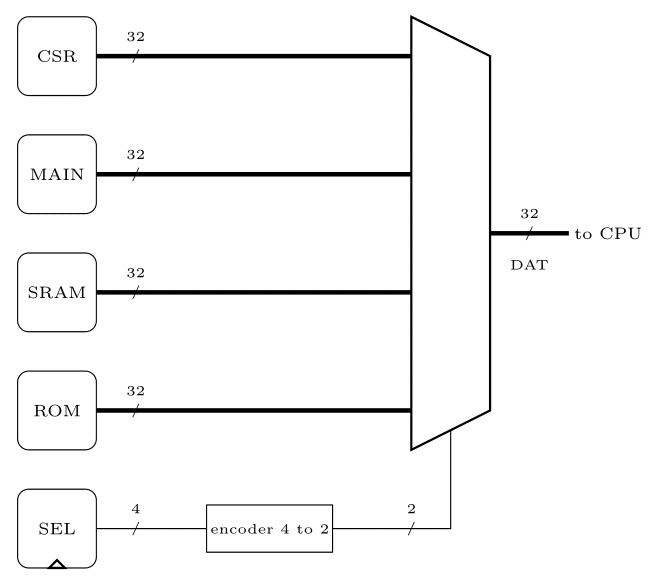
\includegraphics[width=0.9\linewidth]{Chapitre4/figures/change arch.png}
  \caption{Optimized connection between selection register and memory using multiplexers}
  \label{change archi}
\end{figure}

We employed six different countermeasures for the \texttt{ACK} and \texttt{SEL} registers:
\begin{enumerate}
\item Simple Parity: Detects faults using a 1-bit parity code.
\item Duplication: Creates a duplicate of the registers and compares it with the unprotected version. In Figure~\ref{cm archi}, the \texttt{SEL} signal is duplicated after the encoder, and the duplicated 2-bit signal is stored in the \texttt{cm} register. The signals in both registers are then compared to verify the integrity of the \texttt{SEL} signal and ensure it has not been tampered with. The comparison result is subsequently transmitted to the CPU.
\item Complementary Duplication: Duplicates the inverse of the registers and compares it with the unprotected version.
\item Hamming Code: Corrects the output signal of a register using a 3-bit checksum.
\item SECDED Code: Corrects or detects errors using a 4-bit checksum.
\item Triplication: Duplicates a register twice, correcting the signal if two registers have matching outputs and detecting errors if all three differ.
\end{enumerate}

\begin{figure}[t!]
  \centering
  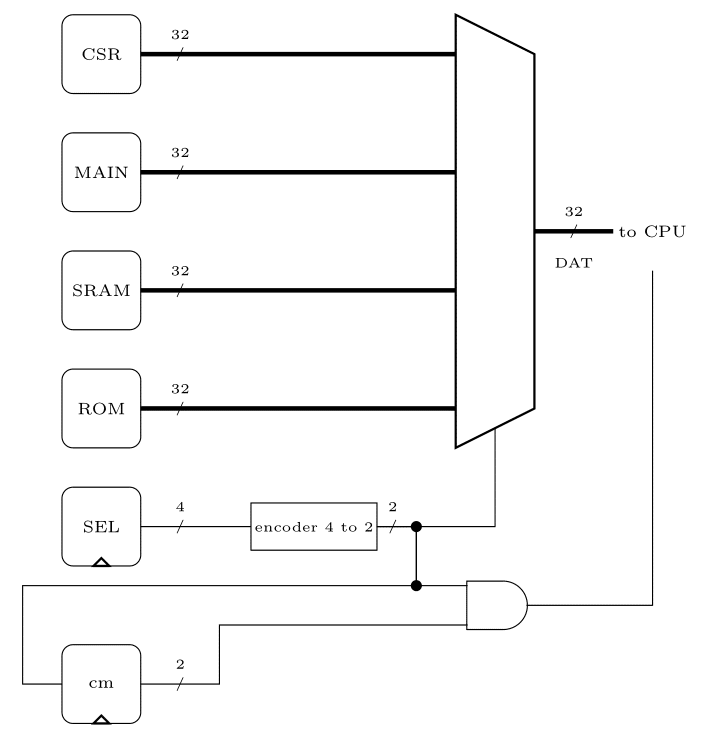
\includegraphics[width=0.9\linewidth]{Chapitre4/figures/cm.png}
  \caption{Structure of selection register and memory after deploying duplication countermeasure}
  \label{cm archi}
\end{figure}

\subsection{Step}
In our Verilog-based implementation, each hardware countermeasure was individually integrated into the \texttt{ACK} and \texttt{SEL} registers, resulting in six distinct project variants. Unlike software defenses, hardware protections function in real time, ensuring that simulation-time variables remain consistent across all configurations. However, introducing additional protection registers inevitably expands the attack surface, as these new elements may also become potential fault targets. To reflect these changes, we modified the register list in the YAML configuration file. We then employed FISSA to regenerate the corresponding TCL scripts and conducted fault injection campaigns using the Quastrasim simulation framework.

We performed a comprehensive analysis of the fault injection outcomes, focusing on several key metrics: the number of distinct fault conditions, attack success rate, detection rate, and correction rate. The experiment was conducted over a period of approximately one week, during which a total of 1,205,604 simulations were executed. Based on this dataset, we systematically compared the performance of different hardware countermeasures across multiple dimensions, as summarized below.

To further evaluate the cost of each countermeasure, we used Vivado to analyze resource utilization. Since resource overhead cannot be directly attributed to individual countermeasures, we synthesized and implemented full SoC designs containing each protection scheme, then compared the resulting differences in overall resource usage.

The experiments were carried out using Vivado version 2024.2 to ensure up-to-date toolchain support and synthesis accuracy. The SoC structure was specified as the top-level module. To obtain precise resource consumption metrics, we used post-implementation resource statistics rather than synthesis-only results. Based on the analysis, we identified and compared key resource categories including LUTs, flip-flops, and timing metrics such as Worst Negative Slack (WNS).

\begin{enumerate}
\item LUT (Look-Up Table): This represents the number of logic elements used to implement combinational logic. LUTs are the fundamental building blocks of FPGA logic, and their count reflects the complexity of the digital logic in the design.
\item Flip-Flop (FF): This indicates the number of sequential storage elements used in the design. Flip-flops store state information and are typically used for registers, control logic, and pipelines. The flip-flop count reflects the degree of sequential logic and pipelining.
\item WNS (Worst Negative Slack): This is a timing metric that shows the most critical timing violation, if any. A negative WNS means the design fails to meet timing requirements for at least one path. A positive or zero WNS indicates that the timing constraints are satisfied. Minimizing or eliminating WNS is essential to ensure reliable operation at the target clock frequency.
\end{enumerate}

Next, we need to calculate the maximum frequency for each structure. We adjust the clock cycle specified in the constraint file in Vivado, then run the implementation to make the WNS parameter closer to zero. The clock cycle obtained in this way is the minimum cycle in the ideal state, which gives us the maximum frequency.
\subsection{Result}

We derive the theoretical upper limit of possible bit-flip faults under the Manipulate Two Registers model, specifically when hardware-level countermeasures such as duplication, triplication, or SECDED are applied. In the most adversarial case, the attacker simultaneously compromises the \texttt{ACK} register (4 bits) and its corresponding redundancy register (4 bits), leading to a total of 8 potential bit-flips. Realistically, inducing such a level of disruption would require the attacker to align two independent fault injection pulses—such as laser beams or electromagnetic bursts—with high spatial and temporal accuracy, targeting both registers in perfect synchrony. As previously documented in the literature, achieving such dual-register precision is highly nontrivial, reinforcing the practical soundness of our threat model.

To evaluate the standalone performance of hardware-based countermeasures, we selected the V0 benchmark as the testing baseline, as it lacks any integrated software protection. The classification criteria for fault outcomes were maintained consistent with prior analysis. Detailed outcomes under varying fault conditions are shown in Table~\ref{tab:v0 under attack result}.

The table reveals significant distinctions in protective performance among the countermeasures. In general, duplication and complementary duplication yield lower attack success rates alongside higher detection probabilities. The Hamming code (SECDED) offers robust correction capability, particularly effective against dual-bit faults and distributed manipulations across two registers. Conversely, triplication is more effective when addressing single-bit errors and multi-bit corruption localized within a single register.

Certain countermeasures are particularly effective against specific attack types:
\begin{enumerate}
\item All countermeasures successfully defend against single bit-flip.
\item Duplication, complementary duplication, and triplication are effective against multi-bit manipulation within a single register.
\item SECDED can defend against two bit-flips.
\item No method can fully prevent multi-bit manipulation across two registers, but triplication performs better.
\end{enumerate}
However, some countermeasures remain vulnerable to specific attacks:
\begin{enumerate}
\item Simple Parity: Highly sensitive to two bit-flips, as simultaneous faults in both the parity and signal lines can compromise its effectiveness.
\item Hamming code and SECDED: Vulnerable to attacks that manipulate two registers, as large numbers of bit alterations can cause false corrections or mask faults in both the signal and the countermeasure.
\item Duplication, complementary duplication, and triplication: Susceptible to two bit-flips since injecting faults into two bits can mirror errors in the complement or duplicate registers, bypassing detection.
\end{enumerate}

\begin{table}
  \caption{Success, detection, and correction rates of hardware countermeasures in V0 benchmark under different fault models}
  \label{tab:v0 under attack result}
{%\footnotesize
\scriptsize
\begin{tabular}{llccl}
\hline
 &  & success rate & detect. rate & correct rate \\
\multirow{-2}{*}{countermeasure} & \multirow{-2}{*}{fault model} & (in \%) &(in \%) & (in \%)\\
\hline
 & bit-flip & 0.93 & &  \\
 & manipulate reg & 0.38 & & \\
 & 2 bit-flips & 1.39 & & \\
\multirow{-4}{*}{Unprotected} & manipulate 2 regs  & 0.71  &  & \\
\hline
 & bit-flip & 0 & 69.85 & \\
 & manipulate reg & 0.02 & 34.93 & \\
 & 2 bit-flips & 0.57 & 64.96 & \\
\multirow{-4}{*}{Simple parity} & manipulate 2 regs & 0.16 & 50.70 & \\
\hline
 & bit-flip & 0 & 77.89 & \\
 & manipulate reg & 0 & 45.11 & \\
 & 2 bit-flips & 0.10 & 86.87 & \\
\multirow{-4}{*}{Duplication} & manipulate 2 regs & 0.03 & 66.78 & \\
\hline
 & bit-flip & 0 & 77.89 & \\
Complimentary & manipulate reg & 0 & 45.11 & \\
duplication & 2 bit-flips & 0.10 & 86.87 & \\
 & manipulate 2 regs & 0.03 & 66.78 & \\
\hline
 & bit-flip & 0 & & 80 \\
 & manipulate reg & 0.31 & & 59.18 \\
 & 2 bit-flips & 0.62 & & 93.28 \\
\multirow{-4}{*}{Hamming code} & manipulate 2 regs & 0.64 & & 77.99 \\
\hline
 & bit-flip & 0 & 0 & 85.71 \\
 & manipulate reg & 0 & 0 & 81.82 \\
 & 2 bit-flips & 0.14 & 20 & 77.40 \\
\multirow{-4}{*}{Triplication} & manipulate 2 regs & 0.09 & 36.73 & 59.24 \\
\hline
 & bit-flip & 0 & 11.76 & 70.59 \\
 & manipulate reg & 0.21 & 34 & 38.56 \\
 & 2 bit-flips & 0 & 45.56 & 52.06 \\
\multirow{-4}{*}{Secded code} & manipulate 2 regs & 0.27 & 51.94 & 36.20 \\
\hline
\end{tabular}
}
\end{table}

The synthesis result is in Table~\ref{tab:countermeasures synthesis}. First, we observe that various countermeasures increase LUT usage by up to 0.7\% and reduce frequency by up to 0.97\% compared to the unprotected version. Considering the difference introduced by the synthesizer's auto-optimization, the countermeasure brings almost no additional hardware resource loss.

\begin{table}
    \centering
  \caption{Hardware resource overhead of each hardware countermeasure (LUT, flip-flop, frequency)}
  \label{tab:countermeasures synthesis}
\begin{tabular}{cccc}
\hline
countermeasure & LUT & flip-flop & frequency (MHz) \\
\hline
Unprotected & 2198 & 1793 & 70.13 \\
Simple parity & 2214 & 1791 & 70.27 \\
Duplication & 2201 & 1791 & 70.18 \\
Complimentary & 2199 & 1791 & 70.37 \\
Hamming code & 2199 & 1794 & 70.32 \\
Triplication & 2199 & 1791 & 70.27 \\
Secded code & 2193 & 1789 & 69.44 \\
\hline
\end{tabular}
\end{table}

\section{Comparison between hardware/software countermeasures}

\subsection{Aim}
Software countermeasures, while lightweight and resource-efficient, often provide only limited protection against fault attacks. They do not introduce additional hardware overhead, making them attractive for constrained environments, but their effectiveness diminishes when facing low-level or persistent fault models. In contrast, hardware countermeasures offer significantly stronger fault resilience by directly modifying the circuit structure or control flow. However, they come at the cost of increased resource consumption and still may not fully eliminate all attack vectors—especially under sophisticated or high-precision injection scenarios.

Given the limitations of each approach when used independently, we explore the possibility of combining software and hardware countermeasures to achieve a more balanced trade-off between protection capability and resource usage. Specifically, we investigate all possible combinations between the seven software countermeasure versions (V1 through V7) and the six hardware countermeasure implementations. Our goal is to determine whether any hybrid configuration can provide improved fault tolerance compared to standalone defenses, reduce the overall resource footprint compared to hardware-only implementations, or ideally, achieve both simultaneously.

\subsection{Step}
To explore the potential benefits of combining software and hardware countermeasures, we constructed a complete evaluation matrix by pairing seven different initialization files—each embedding a unique version of the software countermeasure—with seven Verilog-based SoC implementations, each integrating a distinct hardware countermeasure. The initialization files contain program code pre-instrumented with the corresponding software protections, while the Verilog projects incorporate hardware-level defenses into the SoC architecture, particularly around critical registers such as \texttt{ACK} and \texttt{SEL}.

For each of the 49 combined configurations, we utilized FISSA to generate the appropriate TCL scripts based on the matched software and hardware setup. Fault injection experiments were carried out using the Quastrasim simulation framework over the span of one month, resulting in over 20 million simulation runs in total.

The results were analyzed based on the number and type of fault conditions observed for each configuration. Key evaluation metrics include the attack success rate, detection rate, and correction rate across varying fault models. In parallel, we used Vivado to assess the hardware resource implications of each combination. The post-implementation reports provided detailed data on LUT usage, flip-flop count, and maximum achievable clock frequency, allowing for a comprehensive comparison of protection effectiveness versus hardware cost.

\subsection{Analysis}
Figure~\ref{hw cmp} displays the attack success rates observed under hardware-only countermeasures, while Figure~\ref{sw cmp} shows the corresponding results for software-only defenses. To facilitate a direct comparison between the two approaches, both bar charts are plotted using a unified vertical axis, with the scale limited to a maximum of 0.02.

When evaluating hardware and software countermeasures separately, it is evident that hardware-based protections consistently achieve lower attack success rates—often reaching zero in specific fault models. By contrast, none of the software countermeasures, including the most advanced version (V7), are able to fully eliminate any vulnerability model.

\begin{figure}[t!]
  \centering
  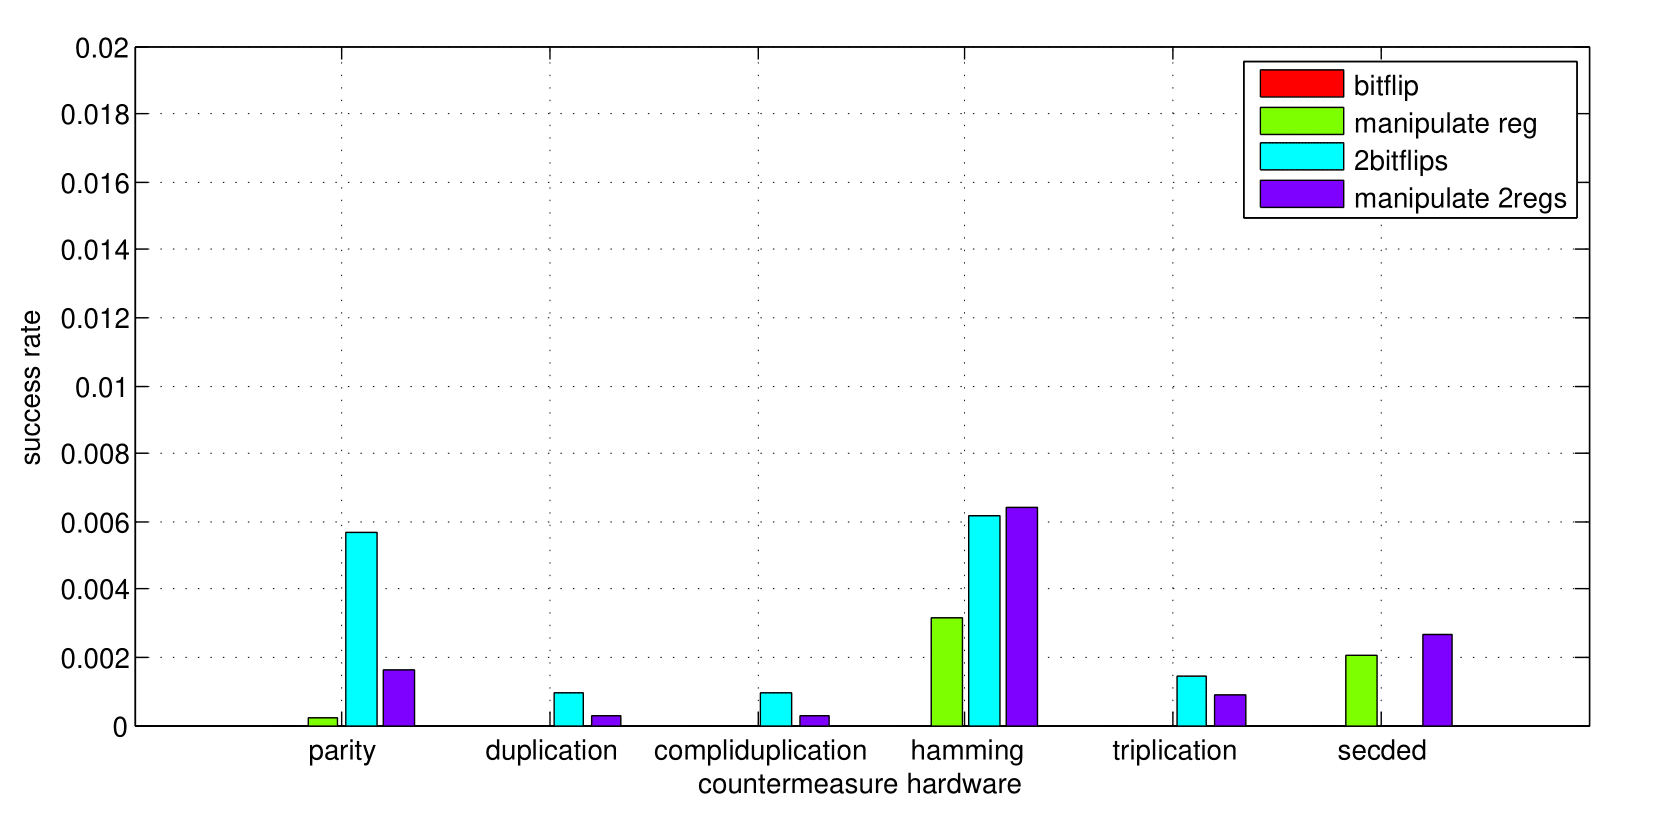
\includegraphics[width=0.99\linewidth]{Chapitre4/figures/hw rate.png}
  \caption{Success rates under four fault models for benchmark v0 with different hardware countermeasures}
  \label{hw cmp}
\end{figure}

\begin{figure}[t!]
  \centering
  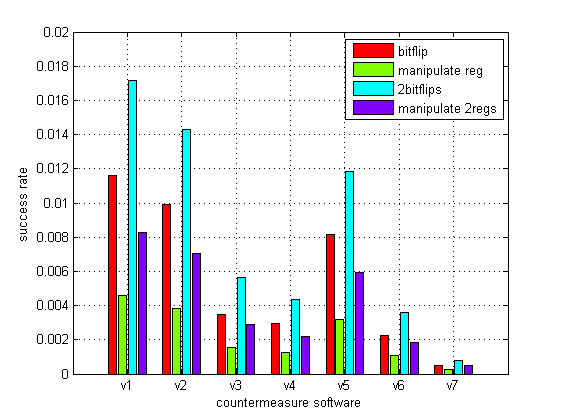
\includegraphics[width=0.99\linewidth]{Chapitre4/figures/sw rate.png}
  \caption{Success rates under four fault models for seven benchmark versions with software countermeasures}
  \label{sw cmp}
\end{figure}

Hardware-based countermeasures are capable of detecting or correcting faults almost instantaneously, with only minimal latency introduced by logic gate propagation delays. In contrast, software-based protections typically require more than 100 clock cycles to complete fault detection. However, considering that the overall program execution spans several thousand cycles, this additional latency is proportionally insignificant.

In terms of resource utilization, hardware countermeasures introduce limited overhead, primarily in the form of extra registers or combinational logic. On the other hand, software countermeasures result in only negligible memory overhead when compared to the total memory footprint of a real-world application. Based on these observations, we conclude that both hardware and software protections incur insignificant overheads—both in terms of execution time and resource consumption—within the scope of our experimental setup.

\begin{table*}
  \centering
  \caption{Success rates of manipulate register attacks on benchmarks with hardware countermeasures}
  \label{tab:manipulate}
\begin{tabular}{lllllllll}
\hline        
& V0 & V1 & V2 & V3 & V4 & V5 & V6 & V7 \\
\hline   
Unprotected                  & 0.385\%                                      & 0.460\%                                       & 0.386\%                                      & 0.153\%                                      & 0.127\%                                      & 0.321\%                                       & 0.108\%                                      & 0.029\%                                       \\
\hline
Simple parity             & 0.019\%                                      & 0.016\%                                       & 0.010\%                                      & 0.012\%                                      & 0.009\%                                      & 0.010\%                                       & 0.011\%                                      & 0.005\%                                        \\
\hline
Duplication               & 0                                              & 0                                              & 0                                              & 0                                              & 0                                              & 0                                              & 0                                              & 0                                              \\
\hline
Complimentary & 0                                              & 0                                              & 0                                              & 0                                              & 0                                              & 0                                              & 0                                              & 0                                              \\
\hline
Hamming code              & 0.314\%                                      & 0.385\%                                       & 0.328\%                                      & 0.120\%                                      & 0.101\%                                      & 0.270\%                                       & 0.081\%                                      & 0.019\%                                              \\
\hline
Triplication              & 0                                              & 0                                              & 0                                              & 0                                              & 0                                              & 0                                              & 0                                              & 0                                              \\
\hline
Secded code               & 0.205\%                                      & 0.255\%                                       & 0.218\%                                      & 0.076\%                                      & 0.065\%                                      & 0.179\%                                       & 0.050\%                                      & 0.037\% \\
\hline
\end{tabular}
\end{table*}

\begin{table*}
  \centering
  \caption{Success rates of 2 bit-flips attacks on benchmarks with hardware countermeasures}
  \label{tab:bitflips}
\begin{tabular}{lrrrrrrrr}
\hline
& V0 & V1 & V2 & V3 & V4 & V5 & V6 & V7 \\
                          \hline
Unprotected                  & 1.391\%                                      & 1.718\%                                       & 1.429\%                                      & 0.564\%                                      & 0.437\%                                       & 1.184\%                                       & 0.358\%                                       & 0.077\%                                       \\
\hline
Simple parity             & 0.567\%                                      & 0.746\%                                       & 0.595\%                                      & 0.254\%                                      & 0.187\%                                      & 0.492\%                                       & 0.159\%                                      & 0.030\%                                       \\
\hline
Duplication               & 0.098\%                                      & 0.122\%                                       & 0.104\%                                      & 0.036\%                                      & 0.031\%                                       & 0.085\%                                       & 0.024\%                                      & 0.005\%                                       \\
\hline
Complimentary & 0.098\%                                      & 0.122\%                                       & 0.104\%                                      & 0.036\%                                      & 0.031\%                                       & 0.085\%                                       & 0.024\%                                      & 0.005\%                                       \\
\hline
Hamming code              & 0.619\%                                      & 0.814\%                                       & 0.647\%                                       & 0.281\%                                      & 0.205\%                                      & 0.535\%                                       & 0.176\%                                      & 0.034\%                                       \\
\hline
Triplication              & 0.147\%                                      & 0.182\%                                       & 0.156\%                                      & 0.055\%                                      & 0.046\%                                      & 0.128\%                                       & 0.036\%                                      & 0.008\%                                       \\
\hline
Secded code               & 0                                              & 0                                              & 0                                              & 0                                              & 0                                              & 0                                              & 0                                              & 0  \\         
\hline
\end{tabular}
\end{table*}

\begin{table*}
  \centering
  \caption{Success rates of manipulate two registers attacks on benchmarks with hardware countermeasures}
  \label{tab:manipulates}
\begin{tabular}{lrrrrrrrr}
\hline
& V0 & V1 & V2 & V3 & V4 & V5 & V6 & V7\\
                          \hline
Unprotected                  & 0.606\%                                       & 0.830\%                                       & 0.703\%                                      & 0.287\%                                      & 0.218\%                                       & 0.591\%                                       & 0.185\%                                       & 0.047\%                                       \\
\hline
Simple parity             & 0.131\%                                      & 0.206\%                                      & 0.162\%                                      & 0.077\%                                      & 0.057\%                                      & 0.136\%                                       & 0.052\%                                      & 0.013\%                                       \\
\hline
Duplication               & 0.021\%                                      & 0.032\%                                       & 0.027\%                                      & 0.010\%                                      & 0.008\%                                      & 0.022\%                                       & 0.007\%                                      & 0.002\%                                       \\
\hline
Complimentary & 0.021\%                                      & 0.032\%                                       & 0.027\%                                      & 0.010\%                                      & 0.008\%                                      & 0.022\%                                       & 0.007\%                                      & 0.002\%                                       \\
\hline
Hamming code              & 0.529\%                                        & 0.787\%                                       & 0.652\%                                      & 0.261\%                                     & 0.207\%                                      & 0.543\%                                       & 0.174\%                                      & 0.042\%                                       \\
\hline
Triplication              & 0.077\%                                      & 0.117\%                                       & 0.090\%                                      & 0.042\%                                      & 0.029\%                                      & 0.075\%                                       & 0.026\%                                      & 0.005\%                                       \\
\hline
Secded code               & 0.227\%                                      & 0.356\%                                       & 0.299\%                                      & 0.113\%                                      & 0.092\%                                      & 0.247\%                                       & 0.074\%                                      & 0.017\% \\  
\hline
\end{tabular}
\end{table*}

When hardware and software countermeasures are combined, several noteworthy observations emerge, as summarized in Tables~\ref{tab:manipulate}, ~\ref{tab:bitflips}, and ~\ref{tab:manipulates}. It is worth noting that, due to the success rate of the bit-flip fault model under hardware-only protection being zero, we omit its graphical representation for clarity.

First, as previously discussed, the effectiveness of hardware countermeasures remains consistent across fault models, regardless of whether software protections are present. This indicates that software integration does not interfere with or alter the baseline performance of hardware-based defenses. Second, when examining the duplication scheme—which has demonstrated the strongest individual performance in mitigating fault attacks—we observe a marked reduction in attack success rates when software protections are layered on top. This improvement is clearly illustrated in Figure~\ref{hwsw combine}, where each version benchmark is compared under two configurations: with duplication countermeasure (shown in azure and purple) and without it (shown in red and green).

However, it is important to highlight that no combination of hardware and software countermeasures is currently capable of fully neutralizing the Manipulate Two Registers fault model. This persistent vulnerability suggests the need for designing more robust or hybridized protection mechanisms that go beyond the current duplication and redundancy paradigms.

\begin{figure}[t!]
  \centering
  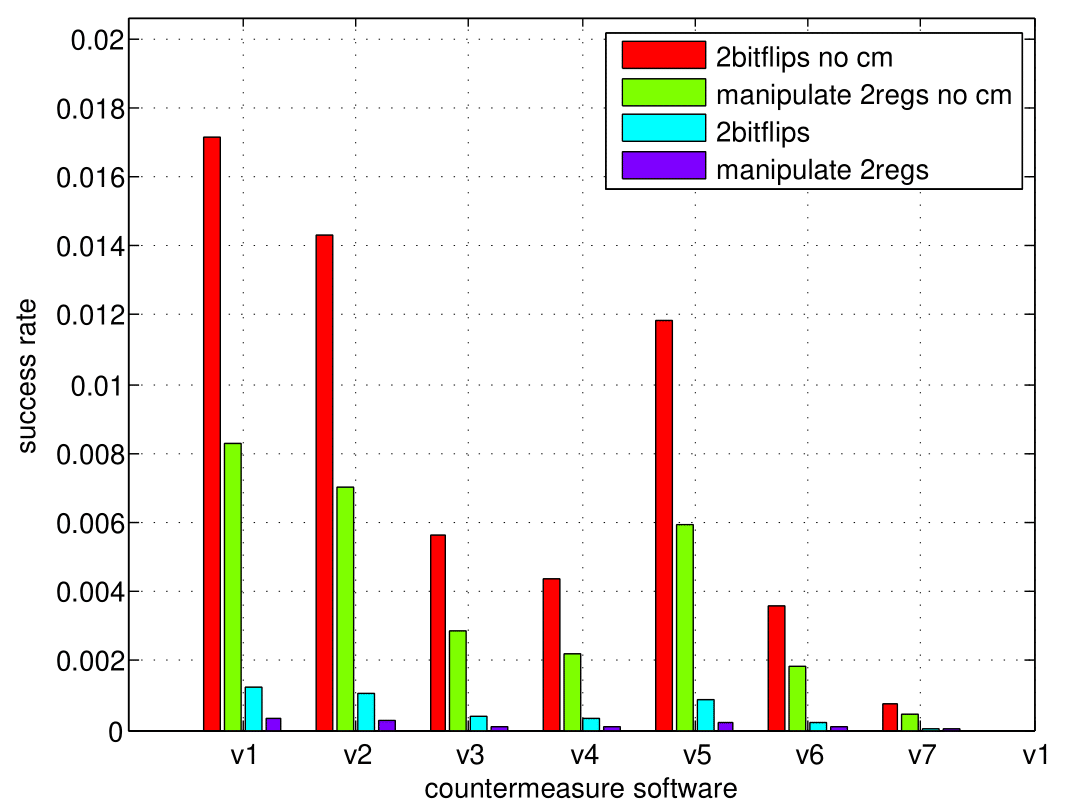
\includegraphics[width=0.99\linewidth]{Chapitre4/figures/duplication.png}
  \caption{Success rates under four fault models for seven benchmark versions with software and/without duplication countermeasures}
  \label{hwsw combine}
\end{figure}

\section{A triple-redundant countermeasure against considered fault models}

\subsection{Aim}
Neither software countermeasures, hardware countermeasures, nor their combination can fully eliminate all fault injection vulnerabilities. This limitation indicates that existing approaches are insufficient for comprehensive protection, and a new, more robust countermeasure must be designed to address all identified fault models effectively.

Among the techniques evaluated, hardware-based protections have shown superior performance in defending against the four fault models introduced in this work. Notably, they achieve this enhanced resilience without imposing significant overhead on hardware resource usage, making them a practical option for real-world deployment. Within the hardware countermeasure category, duplication and triplication architectures consistently outperform other methods, both in terms of reducing attack success rates and maintaining system stability.

Therefore, any future countermeasure design aiming for complete fault coverage should consider drawing on the structural principles of duplication and triplication. These methods provide a promising foundation for developing a more comprehensive and resilient fault-tolerant architecture.
\subsection{Presentation}

To address the four proposed vulnerability models—Bit-Flip, Manipulate Register, Two Bit-Flips, and Manipulate Two Registers—we developed a dedicated hardware-based defense mechanism. As established in our earlier analysis, software protections alone are insufficient to fully mitigate these fault models. Moreover, since no existing hardware countermeasure can comprehensively defend against all of them, we opted for a purely hardware-based solution due to its superior reliability and execution efficiency.

Our investigation also revealed that using hardware solely for fault detection is generally more effective than attempting both detection and correction. Therefore, our design prioritizes high detection accuracy, accepting a modest trade-off in correction capability and performance. The proposed solution follows a hybrid strategy that leverages the structural strengths of both duplication and triplication to form a detection-only triplication-redundant scheme. This mechanism is applied specifically to the selection register and is depicted in Figure~\ref{proposed cm}.

In this design, the output of the \texttt{SEL} register from the encoder is duplicated twice, creating two redundant copies: \texttt{cm1} and \texttt{cm2}. A comparator monitors all three register outputs, and a fault is flagged whenever any discrepancy among them is detected. The same triplication-redundant detection is applied to the \texttt{ACK} register.

\begin{figure}[t!]
  \centering
  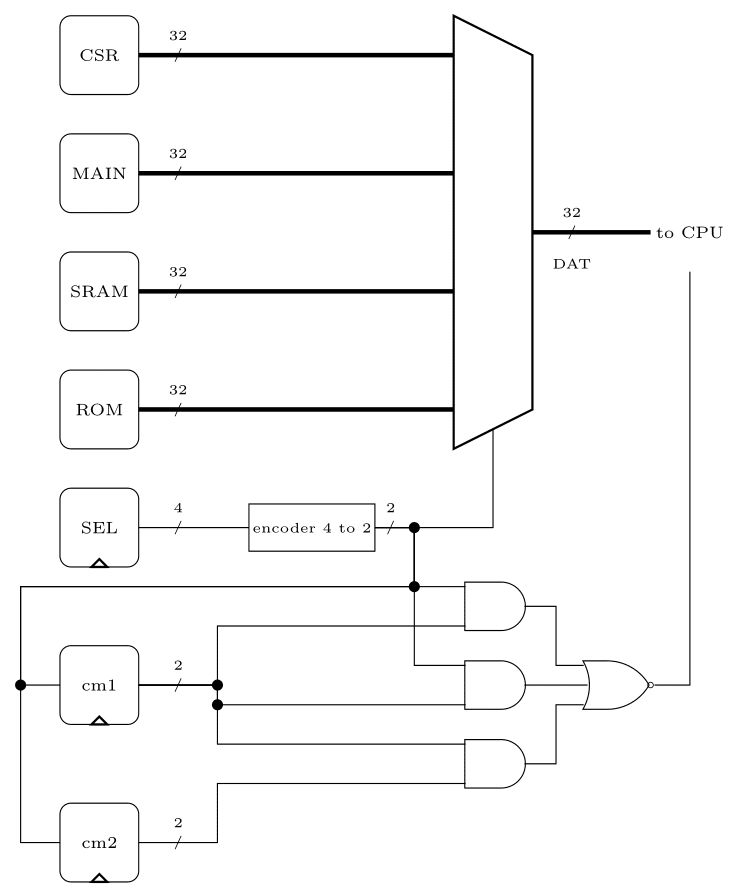
\includegraphics[width=0.9\linewidth]{Chapitre4/figures/cm tri.png}
  \caption{Our proposed countermeasure architecture on the register selection}
  \label{proposed cm}
\end{figure}

\subsection{Analysis}
 As shown in Table~\ref{tab:triplication synthesis}, compared to the baseline system without any protection, our approach increases LUT utilization by only 0.27\% and results in a negligible 0.14\% reduction in maximum clock frequency. Given that our fault model assumes no more than two simultaneously compromised registers, this two-layer redundant detection scheme effectively neutralizes all defined fault scenarios within the model's scope.

\begin{table}
    \centering
  \caption{Hardware resource overhead of Triplication-redundant countermeasure (LUT, flip-flop, frequency)}
  \label{tab:triplication synthesis}
\begin{tabular}{cccc}
\hline
countermeasure & LUT & flip-flop & frequency (MHz) \\
\hline
Unprotected & 2198 & 1793 & 70.13 \\
Triplication-redundant & 2204 & 1791 & 70.03 \\
\hline
\end{tabular}
\end{table}

To validate the robustness of our hardware-based protection, we performed a two-level verification process. First, we verified that the architecture V0 with the proposed countermeasure is resilient to hardware fault injection attacks. Second, we ensured that the architecture, when integrated with seven versions of benchmark variants designed for evaluating software-based countermeasures, also maintains its robustness. We incorporated the proposed countermeasure into all eight versions of benchmark versions under identical experimental conditions. The corresponding results are presented in Table~\ref{tab:our cm}.

\begin{table*}
  \centering
  \caption{Overall attack results on benchmarks with the proposed hardware countermeasure under four fault models}
  \label{tab:our cm}
\begin{tabular}{llrrrrr}
\hline
countermeasure                                                        & fault model      & \multicolumn{1}{c}{crash} & \multicolumn{1}{c}{detect\_hw} & \multicolumn{1}{c}{success} & \multicolumn{1}{c}{change} & \multicolumn{1}{c}{silence} \\
\hline
                                              & bit-flip          & 78                                                & 4138                                                   & 0 & 0                                                   & 698                                                 \\
                                              & manipulate reg   & 113                                               & 4805                                                   & 0 & 0                                                   & 4910                                                \\
                                              & 2 bit-flips        & 1669                                              & 46777                                                  & 0 & 0                                                  & 694                                                 \\
\multirow{-4}{*}{triplication-redundant v0} & manipulate 2 reg & 4527                                              & 140863                                                 & 0 & 0                                                  & 48362                                               \\
\hline
                                              & bit-flip          & 107                                               & 5118                                                   & 0 & 0                                                  & 865                                                 \\
                                              & manipulate reg   & 158                                               & 5937                                                   & 0 & 0                                                  & 6085                                                \\
                                              & 2 bit-flips        & 2290                                              & 57750                                                  & 0 & 0                                                  & 860                                                 \\
\multirow{-4}{*}{triplication-redundant v1} & manipulate 2 reg & 6313                                              & 173872                                                 & 0 & 0                                                  & 59935                                               \\
\hline
                                              & bit-flip          & 147                                               & 8104                                                   & 0 & 0                                                  & 1367                                                \\
                                              & manipulate reg   & 213                                               & 9412                                                   & 0 & 0                                                  & 9611                                                \\
                                              & 2 bit-flips        & 3108                                              & 91712                                                  & 0 & 0                                                  & 1360                                                \\
\multirow{-4}{*}{triplication-redundant v2} & manipulate 2 reg & 8478                                              & 276073                                                 & 0  & 0                                                 & 94673                                               \\
\hline
                                              & bit-flip          & 131                                               & 6956                                                   & 0 & 0                                                  & 1166                                                \\
                                              & manipulate reg   & 186                                               & 8080                                                   & 0 & 0                                                  & 8240                                                \\
                                              & 2 bit-flips        & 2759                                              & 78618                                                  & 0 & 0                                                  & 1153                                                \\
\multirow{-4}{*}{triplication-redundant v3} & manipulate 2 reg & 7402                                              & 236898                                                 & 0 & 0                                                  & 81104                                               \\
\hline
                                              & bit-flip          & 168                                               & 9266                                                   & 0 & 0                                                  & 1570                                                \\
                                              & manipulate reg   & 247                                               & 10759                                                  & 0 & 0                                                  & 11002                                               \\
                                              & 2 bit-flips        & 3553                                              & 104919                                                 & 0 & 0                                                  & 1568                                                \\
\multirow{-4}{*}{triplication-redundant v4} & manipulate 2 reg & 9824                                              & 315618                                                 & 0 & 0                                                  & 108430                                              \\
\hline
                                              & bit-flip          & 150                                               & 7706                                                   & 0 & 0                                                  & 1300                                                \\
                                              & manipulate reg   & 215                                               & 8949                                                   & 0 & 0                                                  & 9148                                                \\
                                              & 2 bit-flips        & 3149                                              & 87119                                                  & 0 & 0                                                  & 1292                                                \\
\multirow{-4}{*}{triplication-redundant v5} & manipulate 2 reg & 8542                                              & 262366                                                 & 0 & 0                                                  & 90100                                               \\
\hline
                                              & bit-flip          & 128                                               & 7102                                                   & 0 & 0                                                  & 1191                                                \\
                                              & manipulate reg   & 182                                               & 8251                                                   & 0 & 0                                                  & 8409                                                \\
                                              & 2 bit-flips        & 2692                                              & 80339                                                  & 0 & 0                                                  & 1179                                                \\
\multirow{-4}{*}{triplication-redundant v6} & manipulate 2 reg & 7235                                              & 242014                                                 & 0  & 0                                                 & 82779                                               \\
\hline
                                              & bit-flip          & 205                                               & 16286                                                  & 0 & 1                                                  & 2745                                                \\
                                              & manipulate reg   & 304                                               & 18935                                                  & 0 & 1                                                 & 19233                                               \\
                                              & 2 bit-flips        & 4405                                              & 185213                                                 & 0 & 2                                                  & 2742                                                \\
\multirow{-4}{*}{triplication-redundant v7} & manipulate 2 reg & 12168                                             & 556725                                                 & 0 & 19                                                 & 189555 \\                               \hline             
\end{tabular}
\end{table*}


In the final phase of our evaluation, the proposed countermeasure was deployed on the \texttt{ACK}, \texttt{SEL}, and \texttt{grant} registers. Due to time limitations, fault injection experiments were conducted only on benchmark versions V0 and V7 of the VerifyPin program. Nevertheless, these two versions are representative enough to validate the effectiveness of the countermeasure.

The results are summarized in Table~\ref{tab:complement}. After extending the countermeasure to cover the \texttt{grant} register, all observed fault injection outcomes were limited to crash, detection, or silence events. Notably, no cases of unintended memory modification were recorded. This provides strong evidence that the proposed countermeasure offers complete protection against all four fault models, irrespective of whether additional software-based protections are applied.

\begin{table}[]
  \centering
  \caption{Attack results on benchmarks with the proposed hardware countermeasure on grant register under four fault models}
  \label{tab:complement}
\begin{tabular}{llrrr}
countermeasure & fault model & \multicolumn{1}{c}{crash} & \multicolumn{1}{c}{detect\_hw} & \multicolumn{1}{c}{slience} \\
\multirow{4}{*}{triplication V0} & bitflip & 78 & 4836 & 468 \\
 & manipulate reg & 113 & 5503 & 5148 \\
 & 2 bitflip & 1825 & 57143 & 234 \\
 & manipulate 2 reg & 4979 & 175435 & 53586 \\
\multirow{4}{*}{triplication V7} & bitflip & 305 & 21808 & 2106 \\
 & manipulate reg & 451 & 24821 & 23166 \\
 & 2 bitflip & 7131 & 258225 & 1053 \\
 & manipulate 2 reg & 19818 & 792045 & 241137
\end{tabular}
\end{table}

\section{Conclusion}
In this chapter, we systematically analyzed and compared the capabilities of software and hardware countermeasures against fault injection attacks (FIAs). Software-based techniques, while offering flexibility and ease of deployment, are often limited by their vulnerability to low-level hardware faults and the constraints of the target environment. To address these shortcomings, we introduced hardware countermeasures grounded in multiplexer hardening and redundancy-based fault masking. By incorporating voting logic and path diversity into critical datapaths, these mechanisms significantly reduce the likelihood of successful fault injection.

A detailed comparison highlighted the trade-offs between software and hardware approaches in terms of coverage, cost, and implementation complexity. While software countermeasures are lightweight and adaptable, hardware solutions offer stronger resilience, especially under repeated or targeted injection scenarios. To bridge this gap, we proposed a triple-redundant countermeasure architecture tailored to the specific fault models observed in our experiments. This design ensures both error detection and recovery by introducing spatial and temporal redundancy at key signal points.

Overall, our findings demonstrate that combining lightweight software-level protections with selective, robust hardware redundancy provides a more balanced and secure defense strategy against practical fault attacks.

Based on these above findings, we offer the following recommendations for RTL-level designers seeking to design secure circuits:
\begin{enumerate}
\item Avoid using combinational logic gates for implementing multiplexers, as this can lead to multiple or no simultaneous reads, introducing vulnerabilities.
\item When hardware complexity are constrained, prioritize detection-only countermeasures and minimize their size, as they provide a lightweight yet effective defense.
\item Be aware of the interactions between software and hardware defenses: While some software defenses may reduce the success rate of hardware attacks, others may inadvertently increase their effectiveness.
\end{enumerate}

\clearemptydoublepage
\backmatter
\chapter{Conclusion}
\chaptermark{Conclusion}
\label{chapter:conclusion}

\epigraph{\textit{The only truly secure system is one that is powered off, cast in a block of concrete and sealed in a lead-lined room with armed guards - and even then I have my doubts.}}{Gene Spafford}

\minitoc

%%%%%%%%%%%%%%%%%%%%%%%%%%%%%%%%%%%%%%%%%%%%%%%%%%%%%%%%%%%%%%%%%%%%%%%%%%%%%%%%%%%%%%%%%%%%%%%
\section{Synthesis}
With the rapid proliferation of embedded systems in safety-critical and high-reliability domains, ensuring their robustness against faults and attacks has become a pressing concern. While traditional protection efforts have focused on computation and storage elements such as CPUs and memory, this work highlights the critical and often overlooked vulnerabilities within on-chip communication architectures—especially system buses.

Through a systematic analysis of three widely used bus protocols—Wishbone, AXI-Lite, and AXI—this study identifies structural weaknesses that can be exploited by fault injection attacks, including those launched via electromagnetic interference. Experimental evidence demonstrates that such attacks can effectively bypass security mechanisms and compromise data integrity, even in systems with strong software-level protections.

To address these challenges, this research proposes a dedicated hardware-based countermeasure for the Wishbone bus architecture. Unlike existing software solutions, our approach integrates fault detection and response mechanisms directly into the bus infrastructure, achieving enhanced resilience without significant performance penalties. Comparative evaluations show that while software countermeasures offer flexibility, they are insufficient in isolation. The proposed hardware solution provides a more comprehensive and robust defense, particularly against persistent and low-level injection strategies.

Based on the discussion in Chapter 1: Attacks, this work establishes a systematic understanding of system-level threats targeting embedded electronic systems. By defining attacks as intentional actions aimed at compromising system security, the chapter structures the threat landscape into two primary categories: hardware-based and software-based attacks. Hardware attacks exploit the physical characteristics of devices through techniques such as reverse engineering, side-channel analysis, hardware Trojans, and fault injection, the latter being especially relevant due to its applicability across abstraction layers from gates to control logic. In contrast, software attacks operate at the logical level, manipulating code, control flow, or memory to trigger unintended behavior or escalate privileges.

A key takeaway from this chapter is the hierarchical nature of vulnerabilities, where low-level physical faults can manifest as high-level software anomalies. This insight reinforces the importance of analyzing security threats across multiple abstraction levels. Furthermore, the chapter surveys a variety of countermeasures—including redundancy, detection mechanisms, desynchronization, and isolation—highlighting the trade-offs between protection strength and implementation complexity. These foundational analyses guide the development of more effective, multi-layered defense strategies throughout the remainder of the thesis.

From Chapter 2: Experiment Setup, this thesis establishes a robust and flexible experimental framework for evaluating fault injection attacks on SoC interconnects. By utilizing LiteX as the base platform, we constructed customizable SoC instances with precise control over bus protocols, memory mapping, and peripheral configurations. This configurability, along with support for both simulation and physical deployment on FPGA platforms, enables scalable and reproducible testing. The framework is built around the VerifyPin benchmark suite, which includes a baseline implementation and seven variants with software countermeasures. VerifyPin simulates a secure PIN verification process, making it suitable for evaluating control flow and memory-level fault impacts.

To conduct systematic fault injection experiments, we adopted the FISSA toolchain, which integrates tightly with HDL simulators such as Questasim. FISSA automates the fault injection workflow, from script generation to simulation execution and log collection, thus enabling high-throughput testing. Within this setup, a realistic black-box attacker model is defined—one without knowledge of the correct PIN ("4321") and using an incorrect input ("0000") to ensure that all successful authentication results arise solely from fault-induced corruption. Faults are injected at the RTL level during the execution of the verifyPIN function, targeting control-related registers over multiple cycles.

To comprehensively evaluate system robustness, multiple fault models are considered. These include single-bit flips, unrestricted bit manipulations within a single register, dual-bit upsets (2-bit flips), and complex simultaneous faults across two distinct registers. Each model reflects practical fault conditions such as those caused by radiation or EM interference. The experimental configuration thus provides a comprehensive basis for analyzing vulnerability patterns and evaluating the effectiveness of both existing and newly proposed countermeasures in subsequent chapters.

From Chapter 3: Vulnerabilities Exploitation on the Bus, this thesis highlights the practical challenges and security implications of conducting fault injection attacks on SoC interconnects. By comparing the behavior of Wishbone, AXI-Lite, and AXI under different fault models, we identified critical vulnerability patterns, particularly in control logic and handshake mechanisms. Our findings emphasize the need for targeted protection of key control signals such as ACK and SEL, as their compromise can lead to severe disruptions including instruction skipping and unauthorized memory access.

The analysis demonstrates that while advanced bus protocols like AXI and AXI-Lite offer structural complexity that may deter simplistic attacks, they simultaneously introduce a broader and less transparent attack surface. In contrast, the Wishbone bus, though more vulnerable due to its simplicity, provides an ideal platform for controlled and precise experimentation. As a result, this study selects Wishbone as the primary target for countermeasure development, enabling focused and reproducible evaluation of protection strategies in the following chapters.

From Chapter 4: Protection Implementation on Wishbone Bus and Test, this thesis presents a comprehensive evaluation of both software and hardware countermeasures aimed at mitigating fault injection attacks on the Wishbone bus. Experimental evidence confirms that vulnerabilities are concentrated around key control signals—specifically the ACK, SEL, and grant registers. Structural weaknesses such as the lack of validation logic, combinational multiplexer paths, and absence of built-in error detection make these elements prime fault targets, capable of leading to successful authentication bypass or instruction-level disruption.

To address these vulnerabilities, the chapter first evaluates the effectiveness of seven software-level countermeasures embedded within the VerifyPin benchmark. While these approaches—ranging from loop counters to step verification—offer moderate resistance against certain attack types, they consistently fail to prevent even simple bit-flip faults when acting alone. This highlights the inherent limitations of software-only solutions, particularly their dependence on the same vulnerable execution context they are designed to protect.

In contrast, six hardware countermeasures—including parity checks, duplication, complementary duplication, Hamming code, SECDED, and triplication—were implemented and analyzed. The results show that hardware-based defenses significantly outperform software approaches, achieving near-zero or zero attack success rates across multiple fault models. Among them, duplication and triplication strategies proved most effective, especially when evaluated under the dual-register manipulation fault model. Furthermore, the overhead introduced by hardware logic remains negligible in terms of resource usage and execution time.

Despite the gains offered by standalone solutions, no individual hardware or software mechanism is capable of eliminating all vulnerabilities. To improve protection coverage, the study explores hybrid combinations of software and hardware countermeasures. While some configurations yield incremental improvements, persistent weaknesses under complex fault models—especially Manipulate Two Registers—underscore the need for more robust design strategies. As a result, a custom triplication-based, detection-only countermeasure is proposed and deployed to the ACK, SEL, and grant signals.

Final testing confirms the effectiveness of this proposed approach: across all conducted experiments using benchmark versions V0 and V7, fault injection results were confined to system crashes, silent failures, or successful detections—with no instances of unauthorized data access or control flow manipulation. These findings demonstrate that the proposed hybrid triplication mechanism offers complete coverage under the evaluated fault models and can serve as a practical, lightweight hardware-hardening strategy for future SoC designs.

Finally, to conclude this part, all the experiments were carried out on a server with the following configuration Xeon Gold 5220 (2.2~GHz, 18C/36T), 128~GB RAM, Ubuntu 20.04.6 LTS and Questasim 10.6e. We ran more than 40 million simulations for all our fault models, and each simulation took an average of 3.29 seconds to run on our server. This totally cost us more than 2 months.

%%%%%%%%%%%%%%%%%%%%%%%%%%%%%%%%%%%%%%%%%%%%%%%%%%%%%%%%%%%%%%%%%%%%%%%%%%%%%%%%%%%%%%%%%%%%%%%
\section{Perspectives}

While our study has successfully identified fault injection vulnerabilities on Wishbone, AXI-Lite, and AXI buses, the scope of implemented countermeasures in this thesis is limited to the Wishbone protocol. This restriction was made primarily for experimental control and reproducibility. However, to achieve a broader understanding of fault resilience across different bus architectures, future research should extend protection strategies—both hardware and software—to AXI-Lite and AXI buses. A comparative evaluation across these protocols would offer deeper insights into the interplay between bus complexity, control logic structure, and countermeasure effectiveness.

On the software side, this thesis primarily employed the VerifyPin benchmark as a representative testbed to analyze fault exploitation and evaluate the impact of software-level countermeasures. While VerifyPin provided a suitable baseline for controlled experimentation, it lacks the diversity and complexity required to generalize results across application scenarios. Future work should involve the implementation of a wider range of software countermeasures—such as control-flow integrity, runtime checks, and execution path verification—within the same SoC framework. These should be tested not only for fault detection capabilities but also for performance overhead, fault coverage, and compatibility with hardware-level protection.

Regarding hardware-based defense, the six protection strategies evaluated in this work—parity checking, duplication, complementary duplication, Hamming coding, SECDED, and triplication—offer a spectrum of trade-offs between complexity and fault tolerance. Nonetheless, numerous alternative mechanisms remain unexplored. For instance, hardware obfuscation, lightweight cryptographic primitives, error-detecting pipelines, and temporal redundancy could offer promising results when integrated into the SoC fabric. Future studies should implement these techniques on the same experimental structure and assess their robustness against realistic and complex fault models, as well as their impact on area, power, and timing constraints.

Finally, while our vulnerability analysis covered three mainstream interconnects—Wishbone, AXI-Lite, and AXI—many other bus architectures are widely deployed in embedded systems and deserve attention. Examples include AMBA AHB, Avalon, TileLink, and proprietary or customized buses used in domain-specific SoCs. Each of these protocols may exhibit unique structural weaknesses and response patterns under fault conditions. A systematic study of these alternatives would broaden the applicability of our findings and support the development of bus-agnostic or protocol-specific countermeasure frameworks.
%%%%%%%%%%%%%%%%%%%%%%%%%%%%%%%%%%%%%%%%%%%%%%%%%%%%%%%%%%%%%%%%%%%%%%%%%%%%%%%%%%%%%%%%%%%%%%%

\clearemptydoublepage
\backmatter
\appendix
% \appendixpage
\input{appendices/appendices}

% Chapitre pour la bibliographie
% Bibliography chapter
\clearemptydoublepage
\phantomsection % To have a correct link in the table of contents
\addcontentsline{toc}{chapter}{Bibliography}

% nocite: Pour citer la totalit\'{e} des r\'{e}f\'{e}rences contenues dans le fichier biblio
% nocite: In order to cite all the references included biblio
\printbibliography

\clearemptydoublepage
% Pour avoir la quatrième de couverture sur une page paire
% To have the back cover on an even page
\cleartoevenpage[\thispagestyle{empty}]
\markboth{}{}
% Plus petite marge du bas pour la quatrième de couverture
% Shorter bottom margin for the back cover
\newgeometry{inner=30mm,outer=20mm,top=40mm,bottom=20mm}

%insertion de l'image de fond du dos (resume)
%background image for resume (back)
\backcoverheader

% Switch font style to back cover style
\selectfontbackcover{ % Font style change is limited to this page using braces, just in case

\titleFR{titre (en fran\c cais)..............}

\keywordsFR{de 3 \`{a} 6 mots clefs}

\abstractFR{Eius populus ab incunabulis primis ad usque pueritiae tempus extremum, quod annis circumcluditur fere trecentis, circummurana pertulit bella, deinde aetatem ingressus adultam post multiplices bellorum aerumnas Alpes transcendit et fretum, in iuvenem erectus et virum ex omni plaga quam orbis ambit inmensus, reportavit laureas et triumphos, iamque vergens in senium et nomine solo aliquotiens vincens ad tranquilliora vitae discessit.
Hoc inmaturo interitu ipse quoque sui pertaesus excessit e vita aetatis nono anno atque vicensimo cum quadriennio imperasset. natus apud Tuscos in Massa Veternensi, patre Constantio Constantini fratre imperatoris, matreque Galla.
Thalassius vero ea tempestate praefectus praetorio praesens ipse quoque adrogantis ingenii, considerans incitationem eius ad multorum augeri discrimina, non maturitate vel consiliis mitigabat, ut aliquotiens celsae potestates iras principum molliverunt, sed adversando iurgandoque cum parum congrueret, eum ad rabiem potius evibrabat, Augustum actus eius exaggerando creberrime
docens, idque, incertum qua mente, ne lateret adfectans. quibus mox Caesar acrius efferatus, velut contumaciae quoddam vexillum altius erigens, sine respectu salutis alienae vel suae ad vertenda opposita instar rapidi fluminis irrevocabili impetu ferebatur.
Hae duae provinciae bello quondam piratico catervis mixtae praedonum.}



\titleEN{titre (en anglais)..............}

\keywordsEN{de 3 \`{a} 6 mots clefs}

\abstractEN{Eius populus ab incunabulis primis ad usque pueritiae tempus extremum, quod annis circumcluditur fere trecentis, circummurana pertulit bella, deinde aetatem ingressus adultam post multiplices bellorum aerumnas Alpes transcendit et fretum, in iuvenem erectus et virum ex omni plaga quam orbis ambit inmensus, reportavit laureas et triumphos, iamque vergens in senium et nomine solo aliquotiens vincens ad tranquilliora vitae discessit.
Hoc inmaturo interitu ipse quoque sui pertaesus excessit e vita aetatis nono anno atque vicensimo cum quadriennio imperasset. natus apud Tuscos in Massa Veternensi, patre Constantio Constantini fratre imperatoris, matreque Galla.
Thalassius vero ea tempestate praefectus praetorio praesens ipse quoque adrogantis ingenii, considerans incitationem eius ad multorum augeri discrimina, non maturitate vel consiliis mitigabat, ut aliquotiens celsae potestates iras principum molliverunt, sed adversando iurgandoque cum parum congrueret, eum ad rabiem potius evibrabat, Augustum actus eius exaggerando creberrime
docens, idque, incertum qua mente, ne lateret adfectans. quibus mox Caesar acrius efferatus, velut contumaciae quoddam vexillum altius erigens, sine respectu salutis alienae vel suae ad vertenda opposita instar rapidi fluminis irrevocabili impetu ferebatur.
Hae duae provinciae bello quondam piratico catervis mixtae praedonum.}

}

% Rétablit les marges d'origines
% Restore original margin settings
\restoregeometry


\end{document}
